\documentclass{tudelft-report}
\usepackage{acronym}
\usepackage{booktabs}
\usepackage{lscape}
\usepackage{gensymb}
\usepackage{textcomp}
\usepackage{multicol}
\usepackage[version=3]{mhchem} % Package for chemical equation typesetting
\usepackage{siunitx} % Provides the \SI{}{} and \si{} command for typesetting SI units
\usepackage{graphicx} % Required for the inclusion of images
\usepackage{natbib} % Required to change bibliography style to APA
\usepackage{amsmath} % Required for some math elements 
%\usepackage[colorlinks=true,linkcolor=blue]{hyperref}
\usepackage{parskip}
\usepackage[nameinlink]{cleveref}
\usepackage[]{caption}
\usepackage{subcaption}


\usepackage{todonotes}
\linespread{1.15}
\newcommand{\todoref}[1]{\todo[backgroundcolor=blue!20!white]{#1}}
\newcommand{\comm}[1]{\todo[backgroundcolor=green!20!white]{#1}}
\setlength{\marginparwidth}{2cm}
\usepackage{titlesec}
\usepackage{sectsty}


\titleformat*{\subsubsection}{\bfseries}

\titleformat*{\paragraph}{\bfseries}
\begin{document}

%% Use Roman numerals for the page numbers of the title pages and table of
%% contents.
\frontmatter

\title[]{Detecting Empty Wireframe Objects on Micro-Air Vehicles \\ { \small Applied for Visual Target Detection in Autonomous Drone Racing}}
\author{P.\ Duernay}
\affiliation{Delft University of Technology}
%\coverimage{cover.jpg}
%\makecover

%% Include an optional title page.
\begin{titlepage}
	
	\begin{center}
		
		%% Insert the TU Delft logo at the bottom of the page.
		\begin{tikzpicture}[remember picture,overlay]
		\node at (current page.south)[anchor=south,inner sep=0pt]{
			
\includegraphics{cover/logo}
		};
		\end{tikzpicture}
		
		%% Extra whitespace at the top.
		\vspace*{2\bigskipamount}
		
		%% Print the title in cyan.
		{\makeatletter
			\titlestyle\color{tudelft-cyan}\Huge\@title
			\makeatother}
		
		%% Print the optional subtitle in black.
		{\makeatletter
			\ifx\@subtitle\undefined\else
			\bigskip
			\titlefont\titleshape\LARGE\@subtitle
			\fi
			\makeatother}
		
		\bigskip
		\bigskip
		
		by
		%door
		
		\bigskip
		\bigskip
		
		%% Print the name of the author.
		{\makeatletter
			\titlefont\Large\bfseries\@author
			\makeatother}
		
		\vfill
		
		in partial fulfillment of the requirements for the degree of
		%in overeenstemming met de vereisten voor het verkrijgen van de graad van
		
		\bigskip
		\bigskip
		
		{\bfseries Master of Science}
		
		in Embedded Systems
		
		\bigskip
		\bigskip
		
		at the Delft University of Technology,
		%aan de Technische Universiteit Delft,
		
		to be defended publicly on Tuesday January 1, 2013 at 10:00 AM.
		%in het openbaar de verdedigen op dinsdag 1 januari om 10:00 uur.
		
		\vfill
		
		\begin{tabular}{lll}
			%% Add additional information here, per faculty requirements, e.g
			%    Student number: & 1234567 \\
			%    Project duration: & \multicolumn{2}{l}{March 1, 2012 -- January 1, 2013} \\
			Supervisor: & Prof.\ dr.\ ir.\ D. M. J\ Tax \\
			Thesis committee:
			& Prof.\ dr.\ C.\ F.\ Guido de Croon, & TU Delft \\
			& Dr.\ E.\ L.\ Brown, & TU Delft \\
			& Ir.\ M.\ Scott, & Acme Corporation
		\end{tabular}
		
		%% Only include the following lines if confidentiality is applicable.
		\bigskip
		\bigskip
		\emph{This thesis is confidential and cannot be made public until December 31, 2013.}
		%\emph{Op dit verslag is geheimhouding van toepassing tot en met 31 december 2013.}
		
		\bigskip
		\bigskip
		An electronic version of this thesis is available at \url{http://repository.tudelft.nl/}.
		%Een elektronische versie van dit verslag is beschikbaar op \url{http://repository.tudelft.nl/}.
		
	\end{center}
	
\end{titlepage}



\chapter*{Preface}
\setheader{Preface}

Preface\ldots


\begin{flushright}
	{\makeatletter\itshape
		\@author \\
		Delft, January 2013
		\makeatother}
\end{flushright}



\tableofcontents

%% Use Arabic numerals for the page numbers of the chapters.
\mainmatter

\chapter*{Summary}
\addcontentsline{toc}{chapter}{Summary}
\setheader{Summary}

\ac{MAV} are an emerging technology that supports a wide range of applications. Thereby the robust estimation of an \ac{MAV}'s state within its environment is crucial to ensure safe operation. In  indoor scenarios cameras are one of the predominant choices for state estimation sensors. This requires Computer Vision algorithms to interpret the obtained high dimensional signal. An application that allows the competitive evaluation of control and state estimation algorithms is \ac{MAV} Racing such as the \ac{IROS}2018 Autonomous Drone Race. Thereby a race court consisting of several race gates has to be followed. For a fast flight during such a race court the detection of the racing gates with a camera can be used in a high level control loop. As these object consist only of small structures that are spread across large parts of the image, this gives rise to a challenging Object Detection problem.

In recent years \acp{CNN} showed promising results on various vision tasks. However, due to their computational complexity the deployment on mobile devices remains a challenge. Furthermore, \acp{CNN} typically require a vast amount of training data. This work defines the class of \acp{EWFO} and studies their detection on \acp{MAV} with \ac{Yolo}V3. For the training, data is generated with a graphical engine. 

The experiments conducted in simulation show how \acp{EWFO} are harder to detect than filled objects as the detector can be confused to patterns present in the empty part. Particularly for larger objects the detection performance decreases. We give several recommendations how to generate data for the detection of \acp{EWFO} on \acp{MAV}. These include how to include variations in background as well as the camera placement. Finally, we study the incorporation of image augmentation techniques to transfer the detector to the real world. We can report that especially modelling lens distortion improves the performance on the real data. Nevertheless, a reality gap remains that can not fully be explained.

Furthermore, different architectures are studied for the detection of \acp{EWFO}. It can be seen how a relatively shallow network of 9 layers can be used for the detection of \acp{EWFO} on \acp{MAV}. A further reduction in weights leads to a gradual decrease in performance. 

Based on the gained insights the deployment of a detector on an example system is studied. A detection performance/speed trade-off is evaluated. The final detector achieves 32\% $ap_{60}$ at a frame rate of 12 Hz on a real world test set created during this work.



\chapter*{Glossary}
\begin{acronym}
	\acro{IR}{Infrared}
	\acro{LIDAR}{Light Detection And Ranging}
	\acro{EWFO}{Empty Wire Frame Objects}
	\acro{FoV}{Field of View}
	\acro{CNN}{Convolutional Neural Network}
	\acro{GPS}{Global Positioning System}
	\acro{GPU}{Graphical Processing Unit}
	\acro{MAV}{Micro-Air Vehicle}
	\acro{DR}{Domain Randomization}
	\acro{TO}{Target Object}
	\acro{DSC}{Depthwise Separable Convolution}
	\acro{IMU}{Inertial Measurement Unit}
	\acrodefplural{IMU}[IMUs]{Inertial Measurement Units}
	\acro{FPV}{First Person View}
	\acro{IROS}{International Conference of Intelligent Robots}
	\acro{i.i.d.}{independently identically distributed}
\end{acronym}
\chapter{Introduction}
\label{sec:intro}
\acresetall
\acp{MAV} such as a Quadrotor-\ac{MAV} displayed in \autoref{fig:mav} are an emerging technology that supports society in a wide range of consumer, industrial and safety applications. For example \acp{MAV} are used to deliver medicine \cite{Shankland2018}, fight fires \cite{KateBaggaley2017} or even find survivors in disaster situations \cite{JoshuaBateman2017}.

\begin{figure}[b]
	\centering
	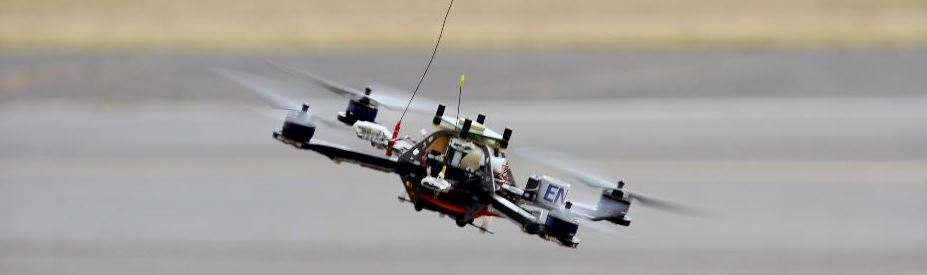
\includegraphics[width=\textwidth]{fig/mav}
	\caption{An example of a Quadrotor-\ac{MAV}-Platform that is used in this thesis.}
	\label{fig:mav}
\end{figure}

Especially in emergency scenarios the fast and safe flight of \acp{MAV} is crucial to deliver help quickly and save human lives. However, due to the complexity of such missions as well as the difficulty to control an \ac{MAV} in disaster scenarios, often multiple human operators are required in order to ensure safe operation \cite{Murphy2016}. With humans in the loop a constant connection between the \ac{MAV} and the operators is required which not only uses energy and requires infrastructure but also significantly increases the reaction time. Enabling \acp{MAV} to fly more autonomously could allow human operators to control more \acp{MAV} and thus to improve the support in emergency situations.

A major challenge on the way to the full autonomous flight of \acp{MAV} is the accurate estimation of the \ac{MAV}'s state within its environment. The system is highly dynamic so position and orientation can change rapidly. At the same time noise introduced by motor vibrations makes the position estimation with only on-board \acp{IMU} too inaccurate \cite{Mohamed2014}. \ac{LIDAR}-sensors can capture long and wide range 3D information but the sensors are typically heavy and require a significant amount of energy. \ac{IR} sensors can cover distance information but are often limited in their \ac{FoV} as well as in their range. External infrastructure like \ac{GPS} and optical tracking systems can provide accurate measurements but there is no guarantee that such systems are present in real world applications. Cameras on the other hand are cheap, lightweight and can measure long range distance information. This makes them a suitable choice as a sensor for on-board state estimation on light \acp{MAV} \cite{Elbanhawi2017}.

However, the signal delivered by the camera is high dimensional and can not directly be interpreted as position or orientation measurements. Computer Vision algorithms are required to interpret the image and extract relevant information. This can be done by designing an algorithm manually or learning the image processing from annotated examples. In particular Deep Learning based methods aim to combine whole Computer Vision pipelines into one mapping that transforms the raw input image into a task dependent output. Experiments have shown how Deep Learning based methods outperform traditional Machine Learning approaches and manually crafted algorithms \cite{Razavian}. This made them the predominant choice for almost any vision task.

The hereby used \acp{CNN} are designed in a hierarchical way, using multiple layers that are evaluated sequentially. An example architecture is displayed in \Cref{fig:cnn_example}. The network transforms an image of size 224x224 from its input (left) to a task dependent output (right). In this case a classification network predicting 1000 class probabilities is displayed. Each layer applies a non-linear transformation for which the parameters are learned during training. By stacking more layers on top of each other (deepening) and increasing the number of nodes $D$ per layer (widening), highly non-linear functions can be modelled. 

Experiments have shown the superior performance of particularly deep/wide models \cite{He, He2015, Szegedy2014, Zagoruyko2016}. However, this model flexibility assumed to be the reason for their superior performance also leads to immense requirements in computational resources. For example a state-of-the-art Computer Vision model \cite{He2015} contains 60.2 million parameters and one inference requires 11.3 billion floating point operations \cite{Tschannen2017}. 

\begin{figure}[bhtp]
	\centering
	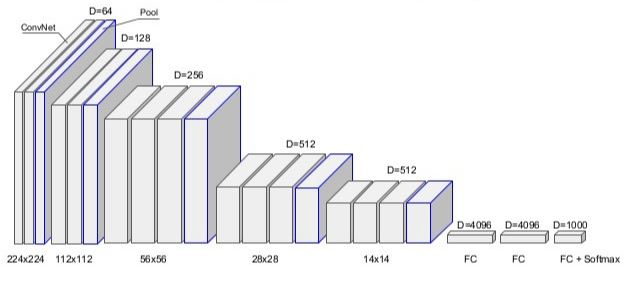
\includegraphics[width=0.8\textwidth]{fig/vgg_architecture}
	\caption{Example Architecture of a \ac{CNN}.}
	\label{fig:cnn_example}
\end{figure}

Robotic platforms like \acp{MAV} have limited resources in terms of processing power and battery life. Hence, the use of \acp{CNN} on such devices is still an open challenge. Research has addressed to reduce the number of computations in Deep Learning models on multiple levels\cite{YoungwanLee, Zagoruyko2016, Howard2017, Ghosh2017, Sandler2018, Zhang2017a}. However, the investigation of relatively shallow models with less than ten layers received only little attention by the research community.

This work investigates the deployment of a Deep Learning based Computer Vision pipeline on a \ac{MAV}. The method is applied in the challenging scenario of Autonomous Drone Racing at the \ac{IROS} 2018. Within the race court several metal gates are placed and need to be passed one after another. Detecting the gates allows to estimate the \ac{MAV}'s relative position and to calculate the flying trajectory. An overview of the race court and the racing gates at the \ac{IROS} 2016 Autonomous Drone Race can be seen in \Cref{fig:race_court}.

\begin{figure}[bhtp]
	\centering
	\begin{minipage}{0.45\linewidth}
	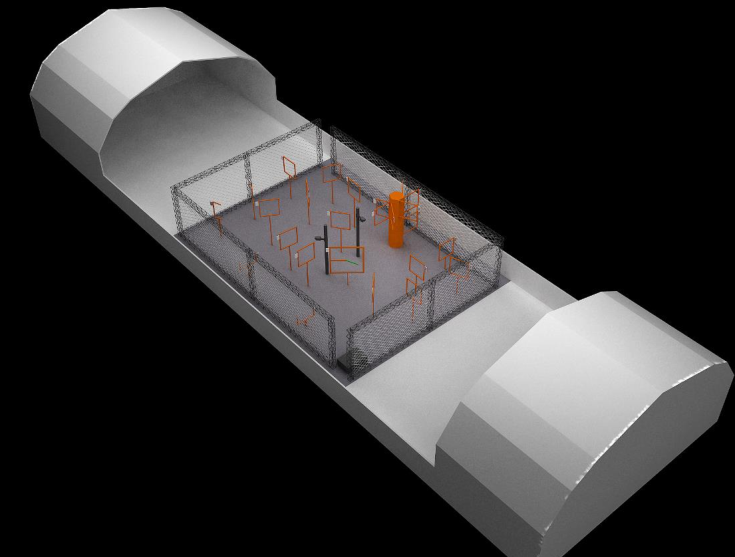
\includegraphics[width=\textwidth]{fig/race_court}
	\end{minipage}\hfill
\begin{minipage}{0.45\linewidth}
	\includegraphics[width=\textwidth]{fig/race_court_side}
\end{minipage}
\caption{Example Images of the \ac{IROS} 2016 Autonomous Drone Race}
\label{fig:race_court}
\end{figure}

The thesis builds on previous work by Ozo et. al \todoref{Reference to Current Method once it is published} which uses a manually crafted image processing method to detect the racing gates. Although fast to execute the method is very sensitive to illumination changes. Moreover, the algorithm fails when the objects are too far away or the frame is very thin. In order to develop a more robust method, this thesis investigates a learning based approach to the detection of racing gates.

Object Detection is one of the most intensively studied topics in Computer Vision. However, the objects investigated are usually solid and contain complex shapes. For example a pedestrian consist of body parts and a face. A box that surrounds the object mostly contains parts with distinctive shape an/or texture. A Computer Vision model can use these features for detection. The racing gates in contrast are of different nature. As can be seen in \Cref{fig:race_court} a box that surrounds the object would largely contain background. Hence, this part can not be used as a hint whether an object is present. Instead it can contain other objects even other gates that might distract a detector. Additionally, the object parts themselves are of very thin structure and can be hardly visible. Thus, a detector needs to make use of fine-grain structures, while ignoring the majority of the image. This introduces a particular vision task that even humans have a hard time at solving \footnote{The unconvinced reader can try to count the number of gates visible in the right image of \Cref{fig:race_court}} and that affects the training and design of a Computer Vision pipeline that aims to detect these kind of objects.

This thesis defines a class of objects as \textbf{\ac{EWFO}} studies methods for their detection. The definition is given as follows:

\paragraph{Definition - Empty Wire Frame Objects}	
\begin{enumerate}
	\item \textbf{Empty.} The object parts are sparse. The bounding box around the object is largely occupied by background.
	\item \textbf{Wire.} The object parts themselves are thin structures. The object does not consist of complex but only basic geometric shapes like corners, lines and edges.
	\item \textbf{Frame.} The object parts can be spread over large parts of the image, while the point of interest is in the center of this part.

\end{enumerate}

The detection of \ac{EWFO} is studied in the examples of the \ac{IROS} drone race gates. These can be seen can be seen in \Cref{fig:gates}. The image shows the \textit{Closed Gate} as well as the \textit{Jungle Gate}. Thereby the orange part is considered to be the object of interest. To the best of the authors knowledge \ac{EWFO} have not been particularly addressed in Computer Vision. In \cite{Falanga} and \cite{Li2018a} the authors also detect racing gates, however the used objects contain more structure than the ones investigated in this thesis. \citeauthor{Jung2018} present a framework to detect similar objects in \cite{Jung} and \cite{Jung2018} but do not study the particular effects of the object shape. This work particularly addresses the implications of the object shape in using a Deep Learning based detection system for \ac{EWFO}.

\begin{figure}[bhtp]
	\centering
	\begin{minipage}{0.45\linewidth}
		\centering
		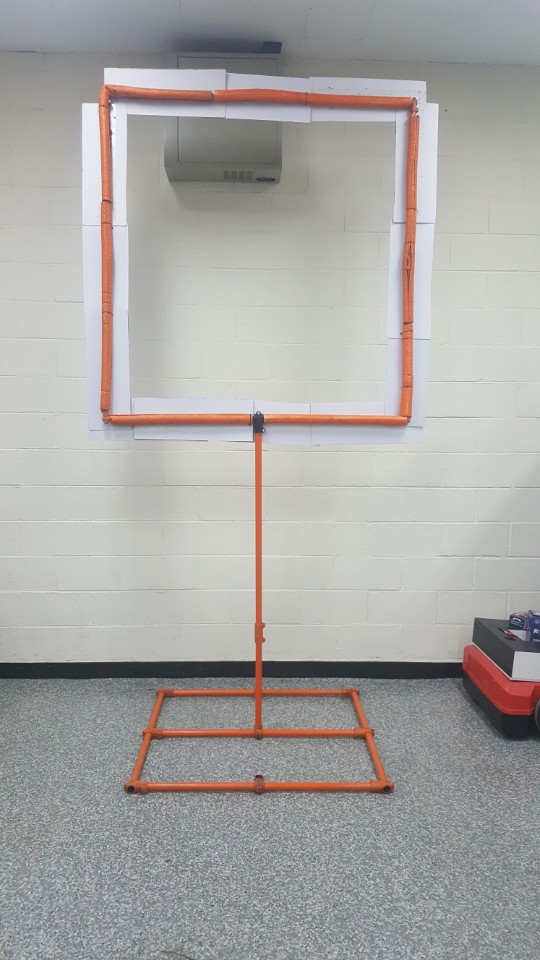
\includegraphics[height=5cm]{fig/closed_real}
	\end{minipage}\hfill
	\begin{minipage}{0.45\linewidth}
		\centering
		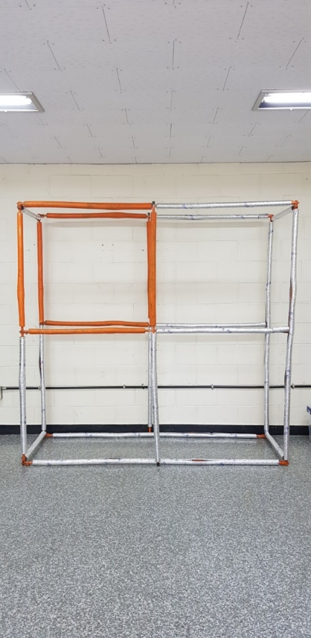
\includegraphics[height=5cm]{fig/jungle_real}
	\end{minipage}
	\caption{Example Images of the Empty Wire Frame Objects investigated in this thesis. }
	\label{fig:gates}
\end{figure}

A drawback of Deep Learning based vision systems is their need for vast amounts of annotated examples, which is not always available. Racing gates for example are not an object that appears often in everyday life and therefore not many example images exist. To this end no publicly available dataset can be used to train a Computer Vision system for \ac{EWFO}. Since a large part of the object consists of background, it is particularly crucial that the training set covers a large variety of backgrounds. Otherwise, it is likely that a model uses the background for prediction and only works in a particular domain (Overfitting). 

\begin{figure}[bhtp]
	\begin{minipage}{0.49\textwidth}
		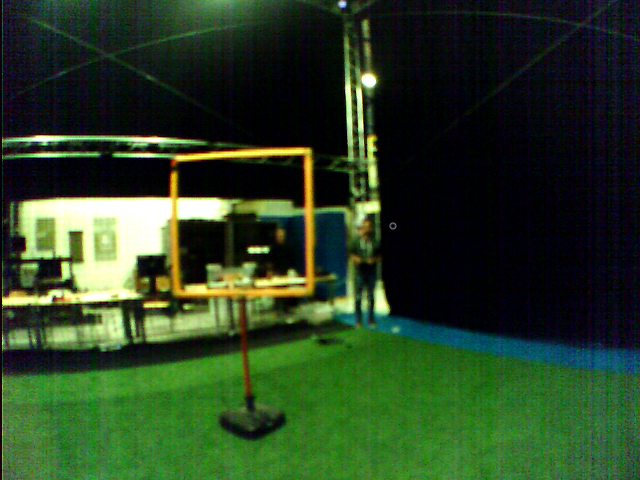
\includegraphics[width=\textwidth]{fig/real_cyberzoo2}
	\end{minipage}
	\begin{minipage}{0.49\textwidth}
		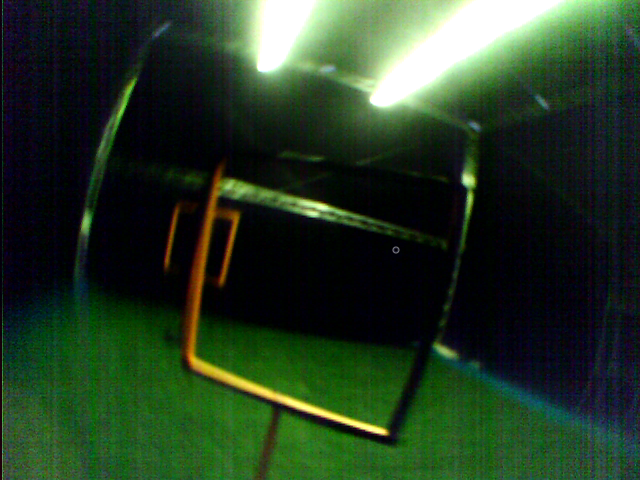
\includegraphics[width=\textwidth]{fig/real_cyberzoo1}
	\end{minipage}
	\label{fig:examples}
	\caption{Example of the \text{Cyberzoo} dataset. On the left an image while the \ac{MAV} is hovering, on the right an image during a turn manoevre.}
\end{figure}

In \Cref{fig:examples} example images of the target domain of this work are displayed. The images are taken during a test flight at a test environment. The left image shows an example when the \ac{MAV} is hovering and thus is in a very stable position. The object in this case is clearly visible as a single orange square. In contrast the right image shows a close up example during a turn manoeuvre. Here it can be seen how the used wide angle lens causes distortion and thus the lines appear as circular shape. Furthermore, large parts of the image including the horizontal bars of the object in the back appear blurred due to the circular velocity of the \ac{MAV}. In addition, the light conditions of the environment significantly influence the object appearance.

While it is possible to remove lens and sensor effects in post-processing, this can lead to information loss and requires on-board resources. Instead it is computationally more efficient to perform the detection on the raw image data. However, sensor effects have been shown to significantly influence the performance of neural networks \cite{Andreopoulos2012,Dodge2016a}. Furthermore, they can lead to varying object appearance on different \acp{MAV}. This further complicates the collection of annotated examples.
 
Another option is the artificial generation of data. By synthetically generating samples with corresponding labels, the theoretical amount of training data is infinite. Moreover, the generation allows to incorporate domain specific properties such as motion blur or image distortion. Hence, data generation is particularly useful for the detection of \acp{MAV} on \acp{EWFO} where a large variety of backgrounds is required while samples are difficult to obtain. Finally, as \ac{MAV} are brittle vehicles and mistakes in development can lead to damage on hardware, engineers and researchers often use simulators to evaluate their systems before transferring them to the real work. Thus the basic infrastructure required to generate data is often already available. 

Yet introduces the generation of data its own challenges. First and foremost because the generation process in itself is based on model assumptions. If these do not sufficiently capture the real world, a model trained in such an environment might be heavily biased and perform poorly in the real world. Secondly, because the generation of visual data is computationally intense. Despite advances in Computer Graphics can virtual environments not yet fully capture the real world. Hence, this work investigates the use of data generation in order to detect \acp{EWFO} on \acp{MAV}.

Without an accurate detection of the racing gate, the \ac{MAV} is not able to determine its current position and thus to calculate its flying trajectory. On the other hand, with an algorithm that requires less computational resources a lighter \ac{MAV} can be built. This allows faster and more aggressive trajectories as well as longer battery life. Moreover, the vision system is part of a greater state estimation and control system which also includes further sensor measurements. Depending on the remaining part of the system, faster and less accurate detections can be more useful than slow but accurate detections. Hence, the trade-off between accuracy and inference speed is of particular interest for this application and is addressed in this work.

\section{Research Question}

This section summarizes the research question addressed in this thesis. Furthermore it describes how the question is split in multiple subquestions that are addressed in the individual chapters.

	\textbf{How can \acp{CNN} detect \ac{EWFO} on \acp{MAV}, using synthetic training data?}


\begin{enumerate}
	\item[\textbf{RQ1}]How can data be generated to train a detection model for \ac{EWFO} detection on a \acp{MAV}?
	\item[\textbf{RQ2}]What kind of architecture is suitable to detect \acp{EWFO}?
	\item[\textbf{RQ3}]What are the trade-offs in detection performance and inference time when a detection model for \acp{EWFO} is deployed on a \ac{MAV}?
	\item[\textbf{RQ4}]Can the gained insights be used to build a lightweight and robust detection model for racing gates in the \ac{IROS} Autonomous Drone Race?
\end{enumerate}

\section{Results/Contributions}

\todo{Put some results at the end.}

\section{Outline}

\todo{Refactor contributions once done}
\begin{figure}[hbtp]
	\centering
	\includegraphics[width=\textwidth]{fig/outline}
	\caption{Thesis Outline}
	\label{fig:outline}
\end{figure}


The thesis is structured as displayed in \Cref{fig:outline}. \Cref{sec:metrics} describes the metrics and systems used for evaluation. \Cref{sec:training}, \Cref{sec:object_detection}, \Cref{sec:tradeoff} and \Cref{sec:method} address the individual research questions. Each chapter contains an introduction to the topic, the methodology used in this thesis and experiments that have been carried out. \Cref{sec:training} describes methods to generate synthetic data for machine learning. It concludes with the datasets used for the remaining parts of this thesis.  \Cref{sec:object_detection} describes object detection and evaluates current methods in the application for \acp{EWFO}. \Cref{sec:tradeoff} illustrates and evaluates measures to reduce computations and optimize an object detection system for a particular hardware. It investigates the trade-off between detection performance and inference time. \Cref{sec:method} describes how the gained insights are used to develop a detector for racing gates at the \ac{IROS} 2018 Autonomous Drone Race. It also compares the current method to a traditional image processing method in terms of speed and detection performance. \Cref{sec:disc} discusses the overall results and formulates a conclusion.




%\chapter{Evaluation Metrics}
\label{sec:evaluation}

\todo{describe metrics and hardware}
\chapter{Background}
\label{sec:background}

This chapter describes background knowledge required to understand the remaining parts of the thesis. It introduces the target system for this work as well as datasets and metrics used for evaluation. Furthermore, it discusses related work in Object Detection and Data Generation.


\section{Detecting Objects}
\label{sec:object_detection:related}

On a high level Object Detection can be described by two individual goals: the description of what kind of object is seen (Classification), as well as where it is seen (Localization). Hence, an Object Detection pipeline transforms the raw image to a set of one or more areas and corresponding class labels. Images are high dimensional signals that can contain redundant and task irrelevant information. Performing detection in this space is difficult, also because the performance of machine learning models decreases when the feature space becomes too large (curse of dimensionality), Computer Vision pipelines usually apply a feature extraction stage, before the actual prediction is done. An overview is displayed in \Cref{fig:obj_pipeline}.

\begin{figure}[hbtp]
	
	\centering
	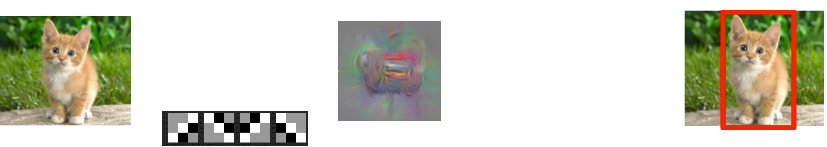
\includegraphics[width=\linewidth]{fig/ObjectDetection}
	\caption{Object Detection Pipeline. An initial step extracts task relevant features of the input signal and derives an internal representation. Consecutively, classification determines what kind of object is present in the image, while localization determines where the object is located. The output consists of area(s) with class annotation.}
	\label{fig:obj_pipeline}
\end{figure}
\begin{enumerate}
	\item The feature extraction stage extracts task relevant information from the image and infers an internal, more abstract representation of lower dimension.
	
	\item The classification/localization stage produces the final output based on this representation. 

\end{enumerate}

An efficient feature extraction stage is thereby crucial for the success of an Object Detection pipeline. If the inferred representation is clearly separable, a simple classification stage can distinguish an object from the background. In contrast, even a flexible classifier cannot separate a highly overlapping feature space.

\subsection{Baseline Algorithm: \textit{SnakeGate}}

The above pipeline can be illustrated in the example of the baseline algorithm of this work: \textit{SnakeGate}. A high level description is given in the following. The interested reader can find more details in \cite{Li2018b}.

Initially, the image gets filtered by a higher and lower color threshold. This way ideally the largest part of pixels in the image is removed. This can be seen as the feature extraction stage.

In the resulting binary image the follow up stage searches for object parts. \textit{SnakeGate} detects square objects and hence looks for vertical and horizontal bars that are respectively perpendicular to each other. Once this combination is found in a particular area of the image, it is counted as a valid detection. In the final step the corners of the bounding box are refined to get more accurate coordinates.

This simple method shows how crucial the feature extraction stage is. With a suitable color threshold, object parts can easily be found and the detection is accurate. However, this requires an evenly distributed colour across the object. As soon as back light or shadows fall on the object, a clear separation is difficult. Therefore, \textit{SnakeGate} is sensitive to light changes.

Another issue of \textit{SnakeGate} is that the object is defined as 4 bars in quadrangle shape. If one of the bars is not clearly visible the algorithm can not detect detect the object. Also, it does not exploit object context such as the object pole. 

\subsection{Related Work}

The problems of \textit{SnakeGate} are very typical for Object Detection. Since the beginning researchers investigated different methods of feature selection and the definition of object models. While initial work manually defined such features, later work replaced many of these stages with learning based methods. Today, whole state-of-the-art pipelines can be trained directly on raw images. This section investigates available literature and discusses the major milestones relevant for this work.

\subsubsection{Traditional Methods}

The early attempts to Object Detection define objects in terms of basic volumetric shapes such as cubes and cylinders. During inference these features are extracted and compared to a database. However, in practice even recognizing these basic shapes proves to be difficult \cite{Andreopoulos2013}. 

Later approaches focus more on appearance based features such as wavelets \cite{Papageorgiou} which also applied in \cite{Viola2004} for human face detection. Thereby the image is processed by a cascade of classifiers using a sliding window in multiple scales. The processing of an image patch is stopped when a patch is classified as background. The features can be computed with simple operations and thus the detector can be executed extremely fast. Yet, the used Haar-wavelets cannot efficiently encode complex textures making the approach less suitable for many real world objects \cite{Andreopoulos2013}. 

In contrast, \ac{HOG} \cite{Dalal} and \ac{SIFT} \cite{Lowe2004} use the image gradient to cover shape information. In a sliding window local histograms based on the gradient orientation are calculated. \citeauthor{Dalal} \cite{Dalal} use the feature for pedestrian detection.

A general challenge in Computer Vision is the combination of local image features such as corners and edges to a more global detection of an object. Especially, when parts of the object can be occluded or deformed and thus undergo variations in appearance. In order to cope with these issues \citeauthor{Felzenszwalb} \cite{Felzenszwalb} model pedestrians in individual parts and combine them in their proposed \ac{DPM}.

Traditional methods have in common that the individual steps of the detection pipeline are optimized separately. Furthermore, often the feature extractors and object models are designed manually. Hence, designing such a detector can result in cumbersome application dependent work. \ac{EWFO} have sparse features and cameras on \ac{MAV} can have a strong influence on the object appearance. Modelling this appearances manually is difficult. Also, the methods seem to have reached a limit in performance in the years of 2005-2012 where almost no improvement in performance was achieved.

\subsubsection{\acp{CNN}-based Feature Extraction}

A breakthrough in detection performance came with \acp{CNN} which emerged from Deep Learning research and subsequently became a popular feature extractor. \acp{CNN} can be seen as small neural networks that are applied locally on image patches in sliding window fashion. The outputs of the initial local operations (first layer) are further processed by higher layers until the desired output size is reached. The model parameters (weights) are trained using a loss function and the back-propagation algorithm.

The modular structure of \acp{CNN} allows to create highly non-linear models that can represent any function. However, this flexibility also introduces the challenge of choosing a suitable architecture. On a fundamental level design parameters can be summarized in depth, width and kernel size. 

\Cref{fig:model_design} displays these parameters and introduces additional terminology necessary for the remaining parts of this chapter. The \textit{kernel size} $\textbf{k}$ determines the spatial size of a kernel and therefore how big the patch is, the convolution is applied on. A layer usually contains multiple filters that are applied on its input. The amount of filters is also referred to as \textit{width} $w$. The filters are applied in sliding window fashion which introduces the step size ( \textit{strides} $\mathbf{s}$) as an additional parameter. The output of each convolution is concatenated and processed by the next layer. The amount of layers is also referred to as \textit{depth}. In the image also the \textit{receptive field} of a filter is visualized. This describes the image patch that is related to a certain feature response. The filter of the first layer (green) has a receptive field corresponding to its kernel size. The filter of the second layer (blue) combines the responses of the filters of the first layer at multiple spatial locations an thus has an increased receptive field.

\begin{figure}[hbtp]
	\centering
	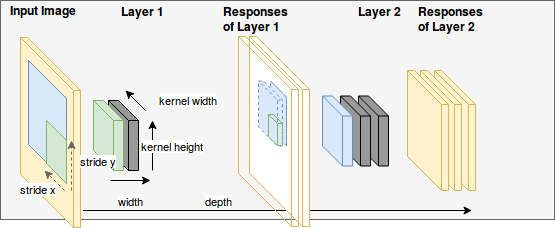
\includegraphics[width=0.8\textwidth]{fig/model_design}
	\label{fig:model_design}
	\caption{Notation in \acp{CNN}. The input image is convolved with a layer. One layer contains multiple kernels that are convolved in sliding window fashion with certain step size. The responses of the convolutions are collected and processed by the next layer. The receptive field is determined by which parts of the input image are part of the kernel response at layer x. The total amount of layers is also referred to as depth.}
\end{figure}

Among these parameters depth is considered one of the preliminary parameters to improve performance \cite{He}. \citeauthor{Simonyan2014} \cite{Simonyan2014} achieve first places in the 2014 ImageNet Classification challenge using a network that only contained filters of size 3-by-3 but up to 19 layers. \citeauthor{Szegedy2014} \cite{Szegedy2014} achieve similar performance using a network with 22 layers. The proposed network included an \textit{Inception}-module, an architectural element that allows deeper networks at a constant computational budget. 

\paragraph{Residual Connections.}

An issue that prevented training even deeper networks is the \textit{vanishing gradient problem}. As the gradient distributes across nodes its magnitude gets smaller with increasing amount of nodes. Hence, the training becomes slow and the risk of converging in a local minima increases. This was addressed by \citeauthor{He2015} \cite{He2015} who propose the use of residual connections. Instead of propagating the gradient from the last to the first layer these connections allow the gradient to flow directly into all layers. This circumvents the vanishing gradient problem. The use of residual connections allowed to train a network 101 layers and improved on state of the art at that time.

\paragraph{Wide-Residual Networks.}

However, later work by \citeauthor{Zagoruyko2016} \cite{Zagoruyko2016} shows how residual networks do not behave like a single deep model but more like an ensemble of more shallow networks. Moreover, the study shows that similar performance can be achieved by particularly wide networks and residual connections. Being of similar performance the proposed \acp{WRN} are computationally more efficient to execute.

While wide residual networks can achieve similar performance to deep residual networks with reduced inference time the computational requirements are still large. This work addresses the detection of \ac{EWFO} with very limited resources. Hence, a network in which the vanishing gradient problem would appear is likely to be already too computationally expensive to be applied on a \ac{MAV}.

\paragraph{Fully Convolution Networks.}

Instead the work focuses on much smaller networks that are fast to execute. Execution time is also the motivation for \acp{FCN}. Instead of using a fully connected layer in the last stage, these networks only apply local operations. This saves many computations in the last layer and enables the application of models on various input sizes.

\paragraph{Dilated Convolutions.}

However, \ac{FCN} in combination with a small amount of layers introduce a limited receptive field. If the network is too shallow the last layer cannot take into account the whole input image. A way to increase the receptive field without increasing the number of computations is the use of sparse kernels, also called Atrous/Dilated convolutions.

\paragraph{Depthwise Separable Convolutions.}

Another line of research to reduce the number of computations in \acp{CNN} address the convolution operation. \textit{MobileNet} \cite{Howard2017} and \textit{QuickNet} \cite{Ghosh2017} make extensive use of \acp{DSC}. \acp{DSC} replace the original 3D-convolution by several 2D-convolutions followed by a pointwise convolution. This reduces the total number of operations from $N = k_w \cdot k_h \cdot w_n \cdot w_{n+1}$ to $N=(k_w \cdot k_h + w_n)+w_n \cdot w_{n+1}$. \textit{MobileNetV2} \cite{Sandler2018} further includes linear bottlenecks to reduce the total number of operations. These are convolutions with a 1by1 kernel and linear activation.

\paragraph{Channel Shuffling.}

In \ac{DSC} pointwise convolutions are the bottleneck. The computation time can be reduced by performing groupwise convolutions. Thereby the channel is separated in subsets and the convolutions are applied on smaller volumes. This reduces computational cost by the number of groups but also stops the information flow between the groups. Therefore \textit{ShuffleNet}\cite{Zhang2017a} proposes a layer that shuffles the channels after the group convolution. This allows the information flow between groups while exploiting the reduced computational cost of group convolutions.

Despite a large amount of research conducted in finding suitable architectures there has not yet been a single way that always achieves a goal. It has been shown how models with a large amount of parameters combined with vast amounts of training data perform well on various vision tasks and objects. However, there is no guarantee that the found representation is also the most suitable/efficient one. The research resulted in a collection of rules an best practices that need to be considered with the task at hand. This work investigates the design of a \ac{CNN} for the detection of \ac{EWFO}.

\subsubsection{\ac{CNN}-based Object Detection}

After showing promising results for Classification, \acp{CNN} where also applied for Object Detection. \acp{CNN}-based Object Detectors can broadly be grouped in two categories. The categories are introduced and finally compared in relevance to this work.

\paragraph{Two-Stage Detectors.}

\citeauthor{Girshick2013} \cite{Girshick2013} use Selective Search \cite{Uijlings2013} to extract object candidates from an image and classify each region with a \ac{CNN}. However, this requires to run the whole network at various scales and overlapping locations. Hence, the approach is computationally intense while many of the performed operations are redundant.

Follow up work aims to share computations for faster inference. Spatial Pyramid Pooling \cite{He2014b} allows to crop any region to a predefined size. Thus a \ac{CNN} does not have to be run at overlapping regions anymore but the extracted features can be reused and need to be only computed once. This leads to a vast reduction in computations and leaves the region proposal algorithm as a computational bottleneck.

With the \ac{RPN}\cite{Ren2015} region proposals and feature extraction is combined in a single stage. The whole stage is framed as a regression problem by predicting object probability for a predefined set of bounding boxes so called anchor/prior or default boxes.  Predefining the total amount of possible locations and bounding box dimensions would lead to an intractable amount of parameters and computations. Hence, the most common object appearances are defined and the network not only predicts an object probability for each box but also how to adapt location and dimensions to better fit the predicted object. Combining feature extraction and region proposals in a single network led to 213x speed up at that time.
 
Being currently the method with the best performance in terms of \ac{mAP} two stage approaches would be a valid choice for the detection of \ac{EWFO}. However, their two stage character makes the inference time relatively slow, which is not suitable for the application on a \ac{MAV}. Also, this work investigates the detection of a single object. For this application the \ac{RPN} can be used directly.

\paragraph{One-Stage Detectors.}

One stage detectors aim to further combine multiple stages of the Object Detection task into a single network. Therefore the whole pipeline is framed as a regression task. This leads to the question how to discretize the input image. 

The first one stage detector \ac{Yolo}\cite{Redmon} divides the input image in a fixed grid and predicts class probabilities for each grid cell. As this limits the amount of bounding box coordinates significantly the network also predicts global bounding box coordinates and a object probability for each box. As a last step a postprocessing algorithm fuses the output to the final prediction. Being a breakthrough as the first one stage detector the approach is limited to predict a single class for each grid cell. Furthermore, the approach of predicting bounding box coordinates globally proved hard for the network to learn and resulted in high localization errors.

Better results could be achieved by predicting offsets to predefined regions as in the concept of the aforementioned anchor boxes. \ac{SSD} \cite{Liu} extends the anchor box approach to perform the whole Object Detection task. Therefore the network not only predicts bounding box coordinate offsets and object probability but also a class probability for each anchor box. 

An issue that arises with discretization of the object detection task is that objects can appear at different scales. For small objects it is required to have a high resolution of bounding box locations to have a sufficient representation of the input image. For example many small objects can appear next to each other. A too coarse resolution could not capture the fact that there are multiple objects present. Furthermore, it is required to take into account fine grain features to predict such an object. In contrast, for large objects small changes in location do not make a difference. In contrary, a too fine resolution can cause the detector focus on noise and thus lead to bad predictions or unstable training. Therefore, \ac{SSD} introduces the prediction of objects at multiple output grids at different layers of the network. Thus, the output grid can be defined depending on the object size and the network can extract features based on the object scale. Follow up work in \cite{Redmon, Redmona} also included the concept of anchor boxes and prediction layers at multiple scales, making \ac{SSD} and \ac{Yolo} converge to a very similar solution.

\if false
A common problem of one stage detectors is the imbalance between background and object samples. Most methods upweigh the positive samples and/or use hard negative mining. \cite{Lin} introduces the \textit{Focal Loss} which focuses on sparse positive samples by design.
\fi

In \cite{Huang} one and two stage detectors are compared in terms of accuracy as well as resource requirements. While two stage detectors with very deep networks tend to achieve the best performance, one stage detectors are generally faster. The experiments also show how the inference time of two stage detectors can be reduced without loosing too much accuracy when the amount of bounding box proposals is limited. However, single shot detectors are still the fastest method with the lowest memory profile. Furthermore, for the single class case the region proposal stage of a two stage detector can be used directly. Hence, in this work we investigate the the detection of a \ac{EWFO} with a one stage detector. The \textit{TinyYoloV3} architecture is 9-layer network with a suitable size to be applied on a \ac{MAV}. This work uses this approach as the baseline model.

The anchor box concept allows to incorporate prior knowledge about possible objects but also introduces additional hyperparameters that need to be tuned for an application. Therefore the alternative approach of \textit{CornerNet}\cite{Law2018} avoids the anchor box concept by defining objects as paired key points. Each bounding box is defined as two corners. The network predicts a heatmap with potential corner locations as well as which corners belong together. This would be an interesting approach for the detection of \ac{EWFO}. However, as the publication was quite recent the approach could not be taken into account. 

\subsubsection{Attention Models}

A research direction which is fundamentally different to the approaches seen so far are models based on visual attention. Instead of processing the whole input image at once, the aim is to process only relevant image patches. Typically a model processes an image crop and decides which location to evaluate next until enough information is gathered for the final prediction. Examples for the approach can be found in \cite{Itti1998,Ba2014,Ablavatski2017a}.

Attention models are promising as their computational complexity can be controlled independently from the number of pixels in the input image. However, to this end successes have mostly been demonstrated on digit recognition like the MNIST dataset. Scaling the approach to real world problems proves to be difficult. Furthermore, the features of an \acp{EWFO} are sparse, while most part of the image does not provide hints where to look for an object. Therefore, we assume the approach less applicable for the detection of \acp{EWFO}.

\section{On the inference time of \acp{CNN}}

For the deployment on a \ac{MAV} resource consumption is an important parameter. Next to the architecture elements such as \ac{DSC} and \textit{Channel Shuffling} other ways are investigated to reduce the inference time of a \ac{CNN}.

\paragraph{Weight Quantization}

Weights are quantized such that the calculations can be performed as integer operations. As \acp{CPU} typically do not have hardware supported floating point units, integer operations can be executed much faster. By mimicking the quantization effects during training, the network learns to deal with these kind of artefacts. 

\paragraph{Knowledge Distillation}

Knowledge Distillation \cite{Hinton2006} is way to create a smaller model based on a trained bigger model or an ensemble of models. Thereby the smaller student-network is trained to mimic the output of the final and intermediate activations of the teacher-network. \textit{FitNet} extends the approach to create a thinner/deeper network based on a trained network thereby reducing parameters without loosing performance. In \cite{Li2017c} the approach is applied to the task of Object Detection. In \cite{Wei2018a} knowledge distillation is combined with weight quantization in order to obtain a faster and more efficient model.

Both methods would be interesting to explore for the deployment of \ac{CNN} on the target system. However, they require an efficient low level implementation. A full implementation of a \acp{CNN} on the target system would be beyond the scope of this work. Therefore the \textit{Darknet}\textit{https://pjreddie.com/darknet/yolo/} framework is used. It supports the hardware available on the target system. Unfortunately, it does not contain the possibility to apply weight quantization or knowledge distillation. Therefore we do not further consider this option and address the inference time on a more architectural basis.

\section{Generating Data}
\label{sec:training:related}

Related methods vary from changing low level properties of the image over using CAD models in combination with real background up to rendering full 3D-environments. Often various combinations of synthesized and real data are applied. 

\subsubsection{Low-Level Image Augmentation}

A common part of current Computer Vision pipelines is to augment a given data set by transforming low level properties of the image. By artificially increasing variations in the input signal, a model that is more invariant to the augmented properties shall be obtained.

\citeauthor{Krizhevsky2012a} \cite{Krizhevsky2012a} use \ac{PCA} to incorporate colour variations. \citeauthor{Howard2013} \cite{Howard2013} shows how several image transformations can improve the performance of a \ac{CNN}-based Classification model. The proposed pipeline includes variations in the crop of the input image as well as variations in brightness, color and contrast. In \ac{CNN}-based Object Detection \citeauthor{Redmon} \cite{Redmon} uses random scaling and translation of the input image, as well as random variations in saturation and exposure. \citeauthor{Liu} \cite{Liu} additionally crop and flip each image with a certain probability.

Since most methods use image augmentation and \citeauthor{Krizhevsky2012a} \cite{Krizhevsky2012a} mentions it to be the particularly reason for superior performance at ILSVRC2012 competition it can be assumed to be beneficial for Computer Vision models. Unfortunately, none of the publications measures the improvements gained by the different operations. 

While the aforementioned approaches add artificial variation to the input data, \citeauthor{Carlson2018}\cite{Carlson2018} augment the image based on a physical camera model. The proposed pipeline is applied for Object Detection and incorporates models for sensor and lens effects like chromatic aberration, blur, exposure and noise. While being of minor effect for the augmentation of real data (0.1\% - 1.62\% \ac{mAP}70) the reported results show an improvement when training on fully synthesized datasets. Here the reported gains vary between 1.26 and 6.5 \% \ac{mAP}70.

Low-level image augmentation is a comparatively cheap method to increase the variance in a dataset. However, it cannot create totally new samples or view points. Furthermore, it cannot change the scene in which an object is placed. Therefore it needs a sufficiently large base dataset that is augmented. This work addresses the case when no real training data is available. Hence, low-level image augmentation is incorporated in the training process but can not be the only method applied.

\subsubsection{Augmenting Existing Images with CAD - Models}

In order to create new view points \ac{CAD}-models can be used. These models describe 3D-shape of an object and can be placed on existing images to augment or increase a dataset.

\citeauthor{Peng}\cite{Peng} study the use of \ac{CAD}-models in the context of \ac{CNN}-based Object Detection. The authors particularly address how image cues like texture, colour and background affects the detection performance. The experiments show how the used \acp{CNN} are relatively insensitive towards context but use shape as primary, texture and colour as secondary most important features. This enables competitive performance even when the object of interest is placed only on uniformly covered backgrounds. However, the study only covers solid objects such as birds, bicycles and airplanes. \ac{EWFO} are substantially different and we hypothesize that other image cues must be relevant.

\citeauthor{Madaan2017}\cite{Madaan2017} study the segmentation of wires based on synthetic training. As wires similarly to \ac{EWFO} only consist of thin edges, the application is quite close to this work. However, the experiments focus on a single domain, namely sky images and thus the variations in background are comparatively small. We hypothesize that \ac{EWFO} are particularly sensitive to such variations and address the application in multiple domains.

\citeauthor{Hinterstoisser2017} \cite{Hinterstoisser2017} propose to use a base network that has been trained on real images and to continue training on images with \ac{CAD}-models. During training the base network is frozen and only the last layers are updated. The method does not use real data but requires a suitable base network. As most available feature extractors are of a size that is computationally prohibitive for \ac{MAV} the method is not really applicable for this work. 

The use of CAD-models in combination with real backgrounds allows to generate totally new view points for the object of interest. Furthermore, the image background consists of real data and thus the synthetic textures only concern the rendered object. However, the geometric properties like perspective as well as the physical properties like object placement are violated and therefore create an artificial scene. Despite this fact, literature shows that such images can benefit model performance in various cases. Yet, most of the approaches still use real data and/or focus on solid objects with rich textures and complex shape. We hypothesize that since \ac{EWFO} do not provide these kind of structures the results do not apply in the same way. Hence, we incorporate the method to generate data and investigate how it can be applied for the detection of \ac{EWFO}.

\subsubsection{Fully Synthesizing Environments}

A more realistic placement of objects can be achieved when fully synthesizing environments.  The object of interest can be placed according to physical laws, shadows fall correctly and geometric properties of an image are followed. However, if the graphical models do not fully capture the details of real world objects, the generated data might look too artificial.

\citeauthor{Johnson-Roberson2016} \cite{Johnson-Roberson2016} use a powerful graphical engine and a highly detailed environment to train an Object Detection model entirely in simulation. The results show an improvement towards data annotated by humans especially when using vast amounts of simulated data. 

In order to create realistic environments intense manual work is required for the design. In contrast \cite{Sadeghi2016, Tobin2017, Tremblay2018a} use a relatively simple environment but a high degree of randomization to address the reality gap. The aim is to learn an abstract representation by strongly varying textures, light conditions and object locations. \citeauthor{Tobin2017} introduced this technique as \ac{DR}. The drawback of the approach is that a too high degree of randomization may omit pattern in the target domain that could otherwise be exploited by the model. 

This work addresses the generation of data for the detection of \ac{EWFO} on \acp{MAV} in \ac{GPS} denied scenarios. Such scenarios cover a wide range of possible environmental conditions and the images taken from \ac{MAV} cameras are peculiar. Hence the creation of a full environment is investigated in this work. 


\subsection{Transfer Learning}

The field of transfer learning particularly addresses domain shifts in the modelling process. Hence, a common application is the learning from synthetic data.

A common approach in \ac{CNN}-based models is the incorporation of a domain classifier in the model. By augmenting the data with domain labels, the classifier learns to distinguish the two domains. Subsequently a gradient reverse layer is applied and thus the weights are updated in such a way that a domain agnostic representation is learned. Examples of the approach can be found in \cite{Chen2018c, Xu2017}.

While the aforementioned approaches require labelled samples from the target domain, \citeauthor{Peng2017} \cite{Peng2017} propose to include task-irrelevant samples and a source classifier. As a result no samples of the target domain are required.

While transfer learning provides the theoretical framework as well as methods to deal with domain shifts, it does not allow to generate data. Furthermore, it often requires samples of the target domain. This work addresses the case when no real data is used for training. The field is interesting to be incorporated in the data generation pipeline investigated in this thesis but it can not be used as a start off point. Hence, the use of transfer learning in the modelling process is denoted as future work.

\subsection{Generative Adversarial Networks}

\acp{GAN} \cite{Goodfellow2014} are a learning technique to generate new samples. The method uses two models a generator and a discriminator. While the generator generates samples the discriminator aims to distinguish the generated samples from a real dataset. Thereby the training goal of the generator is to maximize the error of the discriminator. Both models are updated with back propagation. The method shows promising results for image transformation or image synthesises but also for audio signals \cite{Creswell2017}. Yet to the authors knowledge \acp{GAN} have not yet been applied to generate samples for Object Detection. Furthermore, the discriminator needs a training set for initialization. As for this work only a small amount of training samples are available, we do not investigate this approach for generating samples to detect \acp{EWFO}.

\section{The target system}

\begin{figure}[hbtp]
	\centering
	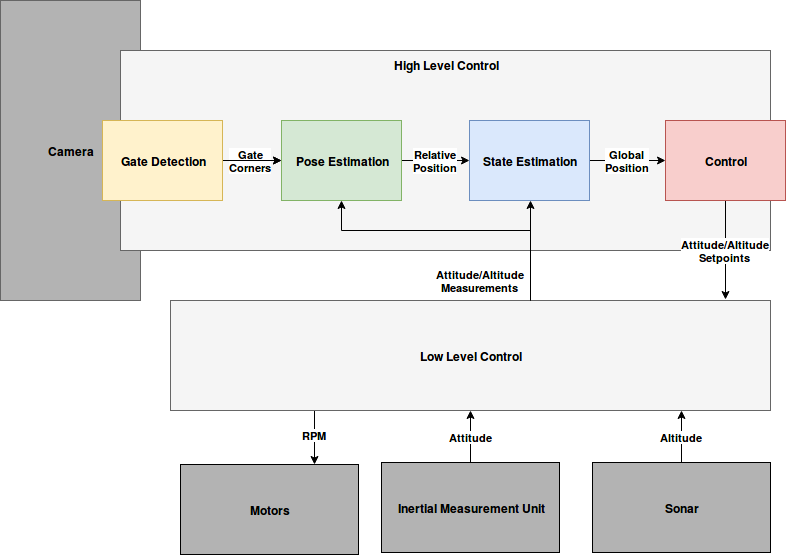
\includegraphics[width=0.8\textwidth]{fig/control_loop}
	\caption{Control Loop}
	\label{fig:control_loop}
\end{figure}

A \ac{MAV} consist of multiple components of Software that are responsible for higher and lower level tasks. \Cref{fig:control_loop} illustrates these components in the example of the target platform of this thesis. On the lowest level drivers read out sensors such as the camera and an \ac{IMU} or communicate with a ground station. A low level control loop is responsible for controlling the local state of the \ac{MAV} such as altitude and attitude. A higher level control loop controls the global state of the \ac{MAV} which is the position and the flying trajectory.

The high level control loop of this work is described in further detail. A first step detects the racing gate and yields the corner coordinates. These are used to estimate the relative position of the \ac{MAV} towards the gate. In the second step the visual measurements are fused with measurements of other sensors. In this case \ac{IMU} and a sonar deliver attitude and altitude data. This step yields a global position estimate of the \ac{MAV}. Combined with prior knowledge about the race court, the desired attitude and altitude required to fly the trajectory is calculated. The results are send as set points to the low level controller.

The hardware platform used to run the high level control loop is the \textit{JeVois} smart camera. It contains a 1.3 MP camera with 65 degree field of view. The processing units are a quad core ARM Cortex A7 processor with 1.35 GHz and a dual core MALI-400 GPU with 233 Mhz. In order to extend the field of view a 120 degree wide angle lens is mounted. In \Cref{fig:jevois} the camera is shown.

\begin{figure}[hbtp]
	\centering
	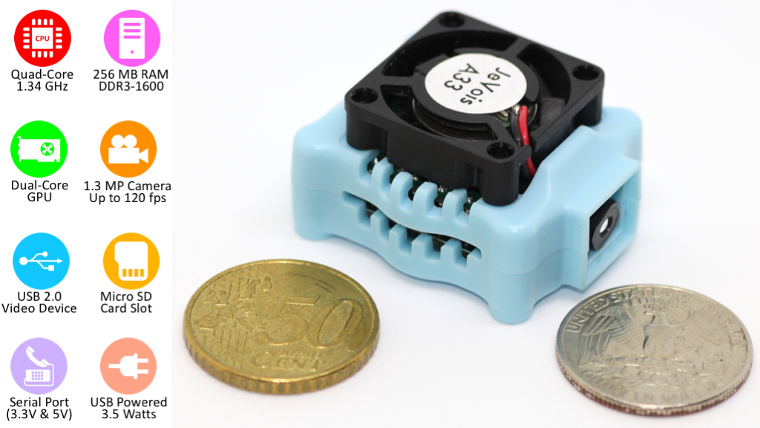
\includegraphics[width=0.5\textwidth]{fig/jevois}
	\caption{JeVois Camera}
	\label{fig:jevois}
\end{figure}



\if false
\section{Baseline}


\subsection{Experiment}

In order to compare the methods investigated in this thesis a baseline is determined. Therefore SnakeGate is evaluated on the datasets described in \Cref{sec:datasets}. In the experiment the color thresholds of the algorithm are fine tuned to the particular environment. The presented results are averages across 5 runs.


\subsection{Results}

The results in terms of precision and recall are summarized in \Cref{fig:snake_results_real}. It can be seen how the detector performs best in the Cyberzoo domain.

\begin{figure}
	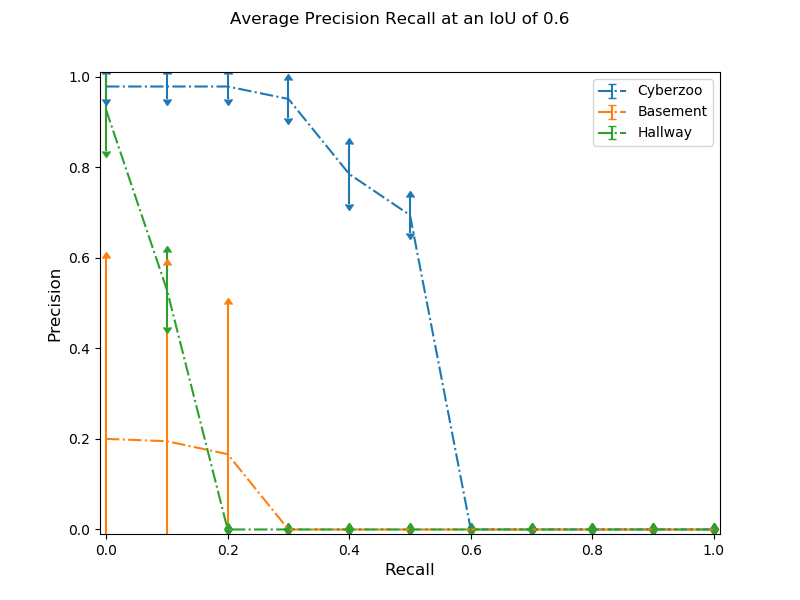
\includegraphics[width=0.8\textwidth]{fig/snake_results_real}
	\caption{Precision-Recall of Snake Gate on the datasets described in \Cref{sec:datasets}}
	\label{fig:snake_results_real}
\end{figure}

\fi
\chapter{Methodology}

\section{Data Generation Pipeline}
\label{sec:datagen:method}
\begin{figure}[htbp]
	\centering
	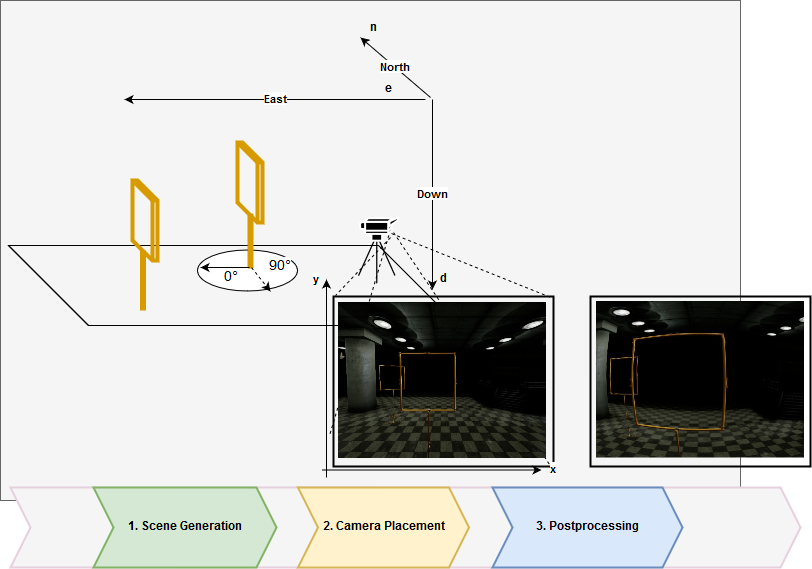
\includegraphics[width=0.9\textwidth]{fig/datagen_notation}
	\caption{Overview of the data generation process.}
	\label{fig:training:datagen_notation}
\end{figure}

A data generation pipeline is implemented using OpenGL, UnrealEngine and AirSim. An overview can be seen in \Cref{fig:training:datagen_notation}. In the first step a scene is created in which the objects of interest as well as the camera are placed. In 3D space position and orientation (pose) of each object are determined by translation $\textbf{t}$ and rotation $\textbf{r}$. The coordinate system is \ac{NED}.

A view projection yields an image through the lens of the camera. The coordinates of each point in 3D space are projected on the 2D image plane. A final post processing step can simulate further effects like lens distortion and sensor noise. This step is implemented using OpenCV and Python. All source code is made publicly available at \url{https://github.com/phildue/datagen.git}.

\subsection{Environments}

Within the pipeline environments for training and testing are created. A black environment serves as base to replace the background with existing images. Furthermore, three indoor base environments are created that fully simulate illumination and background. An overview can be seen in \Cref{fig:environments}. Within the environment light conditions, background textures, object locations can be changed manually. The environments are described in the following:

\begin{enumerate}
	\item \textit{Dark:} The environment is a room without windows, only containing artificial light sources. 
	\item \textit{Daylight:} The environment is a room with windows along all walls that allow daylight to illuminate the room. The windows can lead to strong variations in the contrast between different parts of the object.
	\item \textit{IROS:} The environment resembles the room of the \ac{IROS} Autonomous Drone Race 2018. The light sources stem from a window front at one side of the room, as well as artificial light sources at the ceiling. Depending on the view point, the object might appear against bright or dark background.
\end{enumerate}

\begin{figure}[hbtp]
	\centering
	\begin{minipage}{0.3\textwidth}
		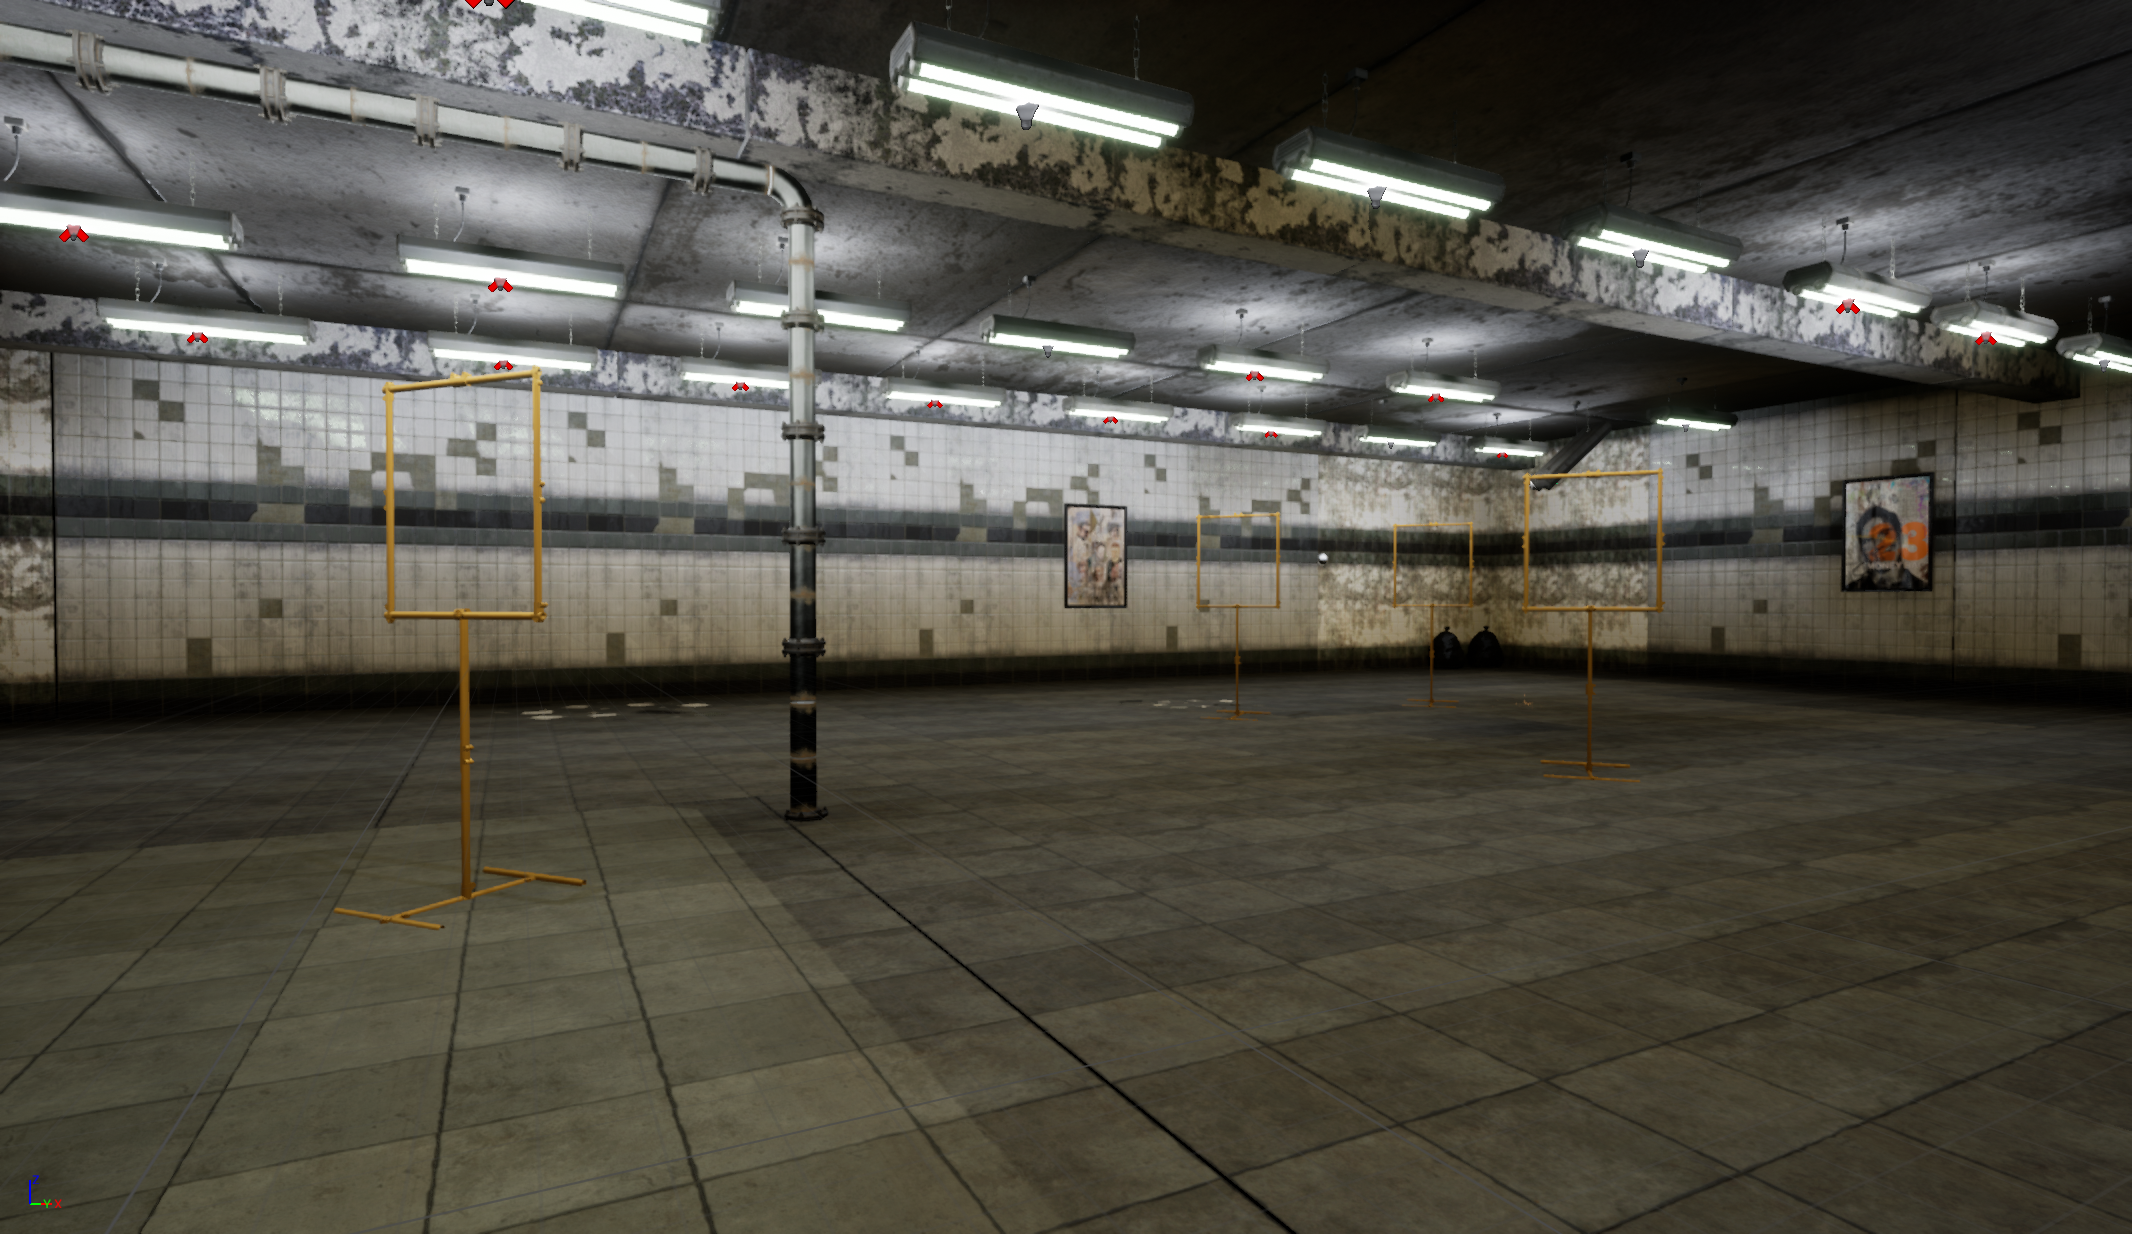
\includegraphics[width=\textwidth]{fig/basement_perspective}
	\end{minipage}
	\begin{minipage}{0.3\textwidth}
		\includegraphics[width=\textwidth]{fig/daylight_perspective}
	\end{minipage}
	\begin{minipage}{0.3\textwidth}
		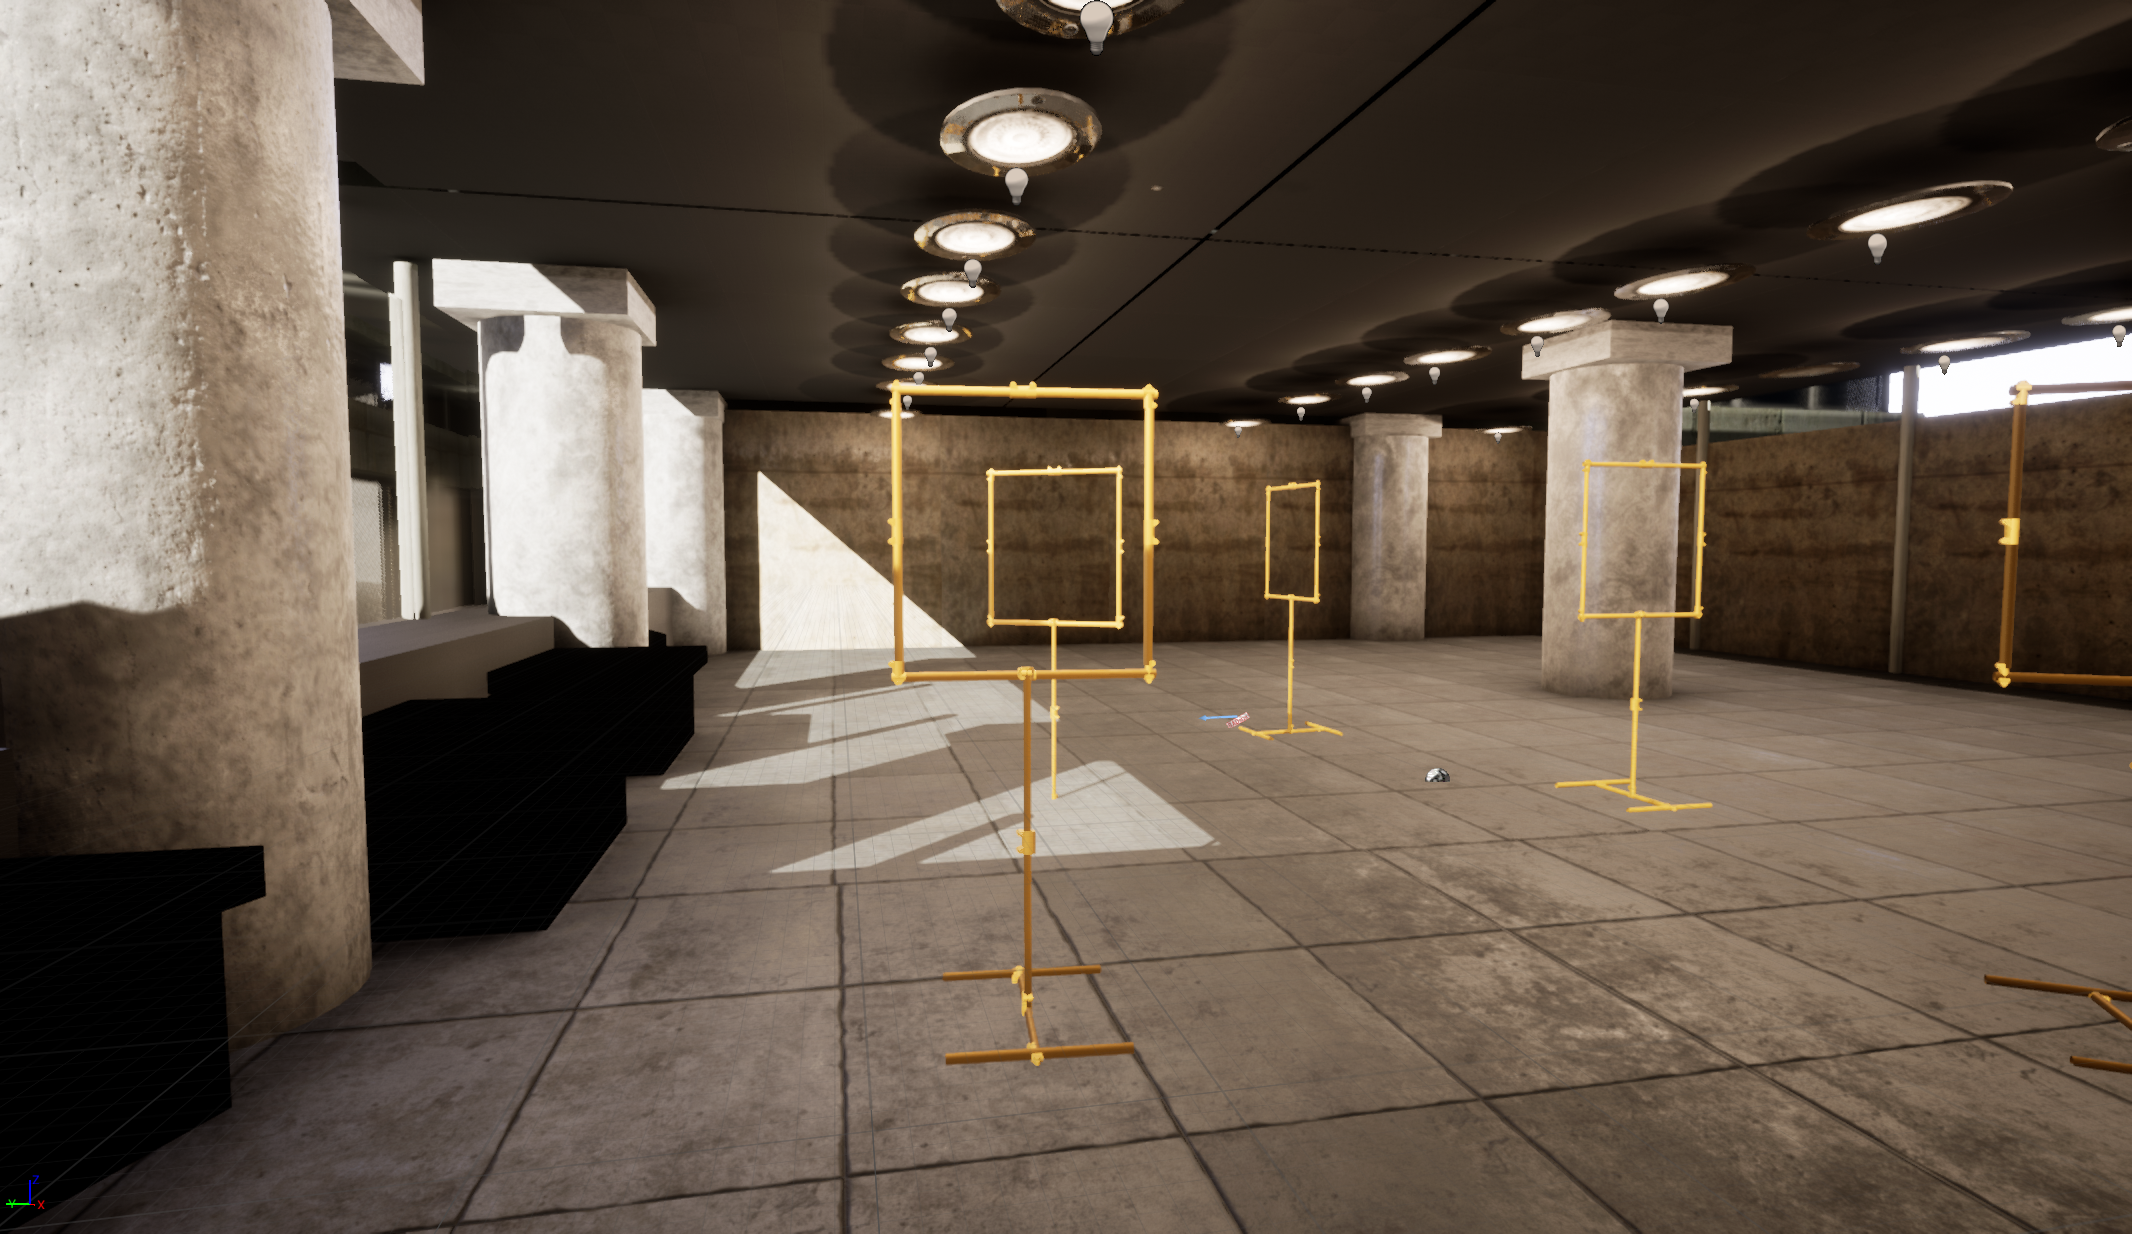
\includegraphics[width=\textwidth]{fig/iros_perspective}
	\end{minipage}
	\caption{The environments from left to right \textit{Dark}, \textit{Daylight}, \textit{IROS2018}}
	\label{fig:environments}
\end{figure}

The data generation pipeline is used to generate a test set in simulation. The test set is set up in the \textit{IROS} environment and inspired by the race court of the \ac{IROS} Autonomous Drone Race. The AirSim flight controller is used to simulate a flight of an \ac{MAV} through the race court. The test set contains 550 images with a total of 1361\todo{recount with filtered} objects.

It should be noted that when generating data with the described methods it is likely that samples appear in which only a corner of the object is visible or the view angle is in such a way that the object appears only as a thin line. In initial experiments these corner cases led to unstable training. Hence, some minimum requirements for the labels are set and samples/labels are removed if these are not met. Objects have to have a minimum size of 1\% of the image area as well as an aspect ratio between 1/3 and 3/1. Furthermore, at least three corners have to be visible.

The models and training are implemented using the \textit{Keras} framework with \textit{tensorflow}-backend. For all trainings the Adam optimizer is applied using a learning rate of 0.001 for the first 60 epochs and a learning rate 0.0001 afterwards. A validation set containing 1\% randomly sampled images from the training set is used. The training is stopped if the validation error does not decrease for more than 5 epochs or 100 epochs are reached.

Throughout the experiments the baseline TinyYoloV3 architecture is used. Thereby we simplify the loss function to a single class prediction. The exact model is described in \Cref{sec:object_detection}. The input image resolution is 416x416.

\subsection{Image Augmentation}

The final step applies low-level image transformations. It allows to further simulate sensor effects and increase the variance in the generated data.

In literature \cite{Krizhevsky2012a,Howard2013,Redmon,Liu} the application of image augmentation is a common tool to improve the detection performance. The experiments in \cite{Carlson2018} show how the incorporation of sensor effects particularly improves the performance of models learned on fully synthesized data. In the \ac{MAV} domain sensor and lens effects have a significant influence on the obtained sample. Hence, we hypothesize that the incorporation of these effects will improve the performance of the trained models. A total of  five image augmentation techniques are investigated.

\paragraph{Lens Distortion}

Lens distortion is a form of optical aberration which causes light to not fall in a single point but a region of space. For \acp{MAV} commonly used wide-angle lenses, this leads to barrel distortion and thus to straight lines appearing as curves in the image.

For this work a 120 wide angle lens is used. Especially, close objects undergo a strong variation in appearance. Hence, we hypothesize including this effect in the training process will improve the performance on the real world dataset. 

The effect is applied using the model for wide-angle lenses from \cite{Vass}. It models the removal of lens distortion as combination of radial and non-radial part, that is approximated with a second order Taylor expansion:
\todo{double check formula is (y in first line?)}
\begin{equation}
\begin{pmatrix}
x_u \\
y_u  
\end{pmatrix}=
f(x,y) =
\begin{pmatrix}
x (1 + \kappa_1 x^2 + \kappa_1 (1 + \lambda_x) y^2 + \kappa_2(x^2 + y^2)^2) \\
y (1 + \kappa_1 x^2 + \kappa_1 (1 + \lambda_y) y^2 + \kappa_2(x^2 + y^2)^2)
\end{pmatrix} 
\label{eq:distortion}
\end{equation}
Where:
\begin{itemize}
	\item $x_u$ and $y_u$ are the undistorted coordinates.
	\item $\kappa_1$ $\kappa_2$ control the radial distortion 
	\item $\lambda_x$ and $\lambda_y$ control the tangential distortion
\end{itemize}

Applying the lens distortion to an image is done using the inverse of \Cref{eq:distortion}. However, as there is no closed form solution, so the Newton-approximation.

An example with $\kappa_1 = 0.5, \kappa_2 = 0.5$ is displayed in \Cref{fig:distortion}. It can be seen how the previously straight lines appear as circular shape.

\paragraph{Chromatic Aberration.}

Chromatic Aberration is caused when different wavelengths of light do not end up in the same locations of the visual sensor. This leads to a shift in the colour channels of the image.

In \cite{Carlson2018} including chromatic aberration significantly improves the performance of models that are trained on fully synthesized data. Hence, we hypothesizes this will also help for our work.

Similarly to \cite{Carlson2018}, chromatic aberration is applied by scaling the locations of the green channel, as well as applying translations on all channels. The model can be implemented as affine transformation of the pixel locations for each channel:

\begin{equation}
f(x_C,y_C) = \begin{pmatrix}
S & 0 & t_x \\
0 & S & t_y \\
0 & 0 & 1
\end{pmatrix} \begin{pmatrix}
x_C \\
y_C \\
1
\end{pmatrix}
\end{equation}

Where $C$ is one colour channel of the image.

An example is displayed in \Cref{fig:chromatic}. It can be seen how the red and green channel are shifted relative to each other. Thus two bars appear in the image.

\paragraph{Blur}

Fast movement and sensor noise can lead to blurry images. This is particularly present in the domain of \ac{MAV}/Autonomous Drone Racing. Hence, we hypothesize including this effect will improve the detection in the real world. 

The effect is modelled using a Gaussian-filter. The image is convolved with a 2D-kernel build from:

\begin{equation}
k(x,y) = \frac{1}{2\sigma_x\sigma_y\pi}e^{-\frac{1}{2}({\frac{(x-\mu_x)^2}{\sigma_x^2} + \frac{(y-\mu_y)^2}{\sigma_y^2}})}
\end{equation}

Where $\sigma_x$ and $\sigma_y$ are the variance in direction x and y, used to model directional (motion) blur and $\mu_x$, $\mu_y$ are at the kernel center. An example can be seen in \Cref{fig:focusblur}.

\paragraph{Exposure.}

Exposure is the time the sensor records light in order to create an image. Over- and Underexposure are caused when this time is too short or too long, leading to too dark or too bright images.

Cameras typically have Autoexposure-functionality which adapts the exposure time depending on light conditions. However, the adoption is not instant, sudden light changes can lead to over- or underexposure. This particularly applies during a fast flight. Hence, we hypothesize incorporating the effect in the data generation will improve the performance of the trained model. The effect is modelled following \cite{Carlson2018}:

\begin{equation}
f(S) = \frac{255}{1 + e^{-A S}}
\end{equation}
where $A$ is a constant term for contrast and $S$ the exposure.
\todo{whats a}
The image can be re-exposed with:

\begin{equation}
I' = f(S+\Delta S)
\end{equation}

where $S$ is obtained from :
\begin{equation}
S = f^{-1}(I)
\end{equation}

An example for overexposure is displayed in \Cref{fig:exposure}. It can be seen how lighter areas appear particularly light, while dark areas remain dark.

\paragraph{Colour Variations}

The 3D-models and textures used in the simulator are limited and creating a large variation in environments or objects requires manual effort. An alternative method to increase the variation in colour and illumination is a scaling in HSV space. The objects in the real world dataset have a slightly different shape and different colour to the 3D-models of the data generation tool. We hypothesize including variations in HSV space will improve the performance on the real world dataset.

The variations are including with:
\begin{equation}
I^* = f(I) = S I
\end{equation}
Where \textbf{S} is a 3D-vector where each element stems from a uniform distribution. The distributions are:


\begin{figure}[htbp]
	\centering
	\begin{minipage}{0.33\textwidth}
		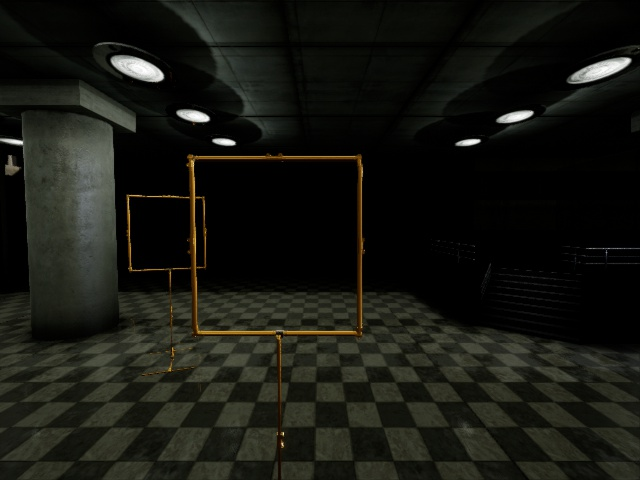
\includegraphics[width=\textwidth]{fig/gate_example}
		\caption{Original Image.}
		\label{fig:orig}
	\end{minipage}
	\begin{minipage}{0.33\textwidth}
		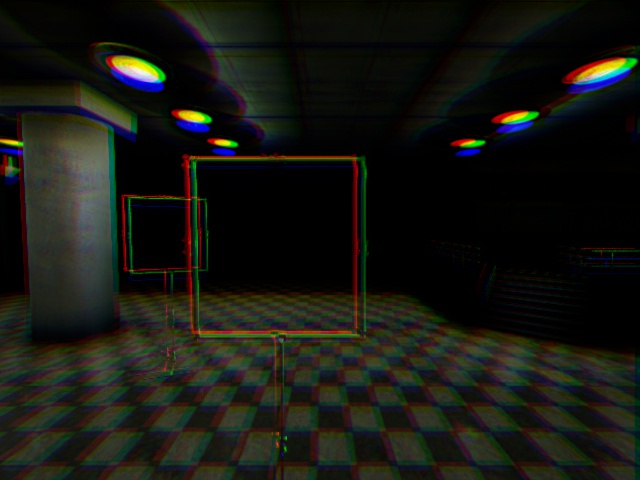
\includegraphics[width=\textwidth]{fig/gate_example_chromatic}
		\caption{Chromatic Aberration.} 		
		\label{fig:chromatic}
	\end{minipage}
	\begin{minipage}{0.33\textwidth}
		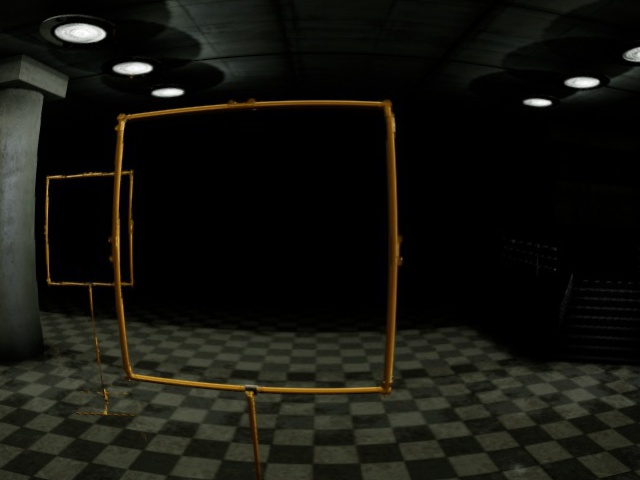
\includegraphics[width=\textwidth]{fig/gate_example_distorted}
		\caption{Lens Distortion. }		
		\label{fig:distortion}
	\end{minipage}
	
	\begin{minipage}{0.33\textwidth}
		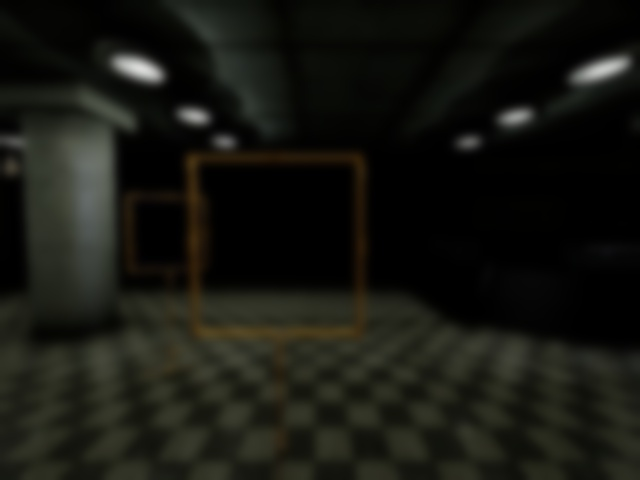
\includegraphics[width=\textwidth]{fig/gate_example_focusblur}
		\caption{Out-of-Focus blur.}
		\label{fig:focusblur}
	\end{minipage}
	\begin{minipage}{0.33\textwidth}
		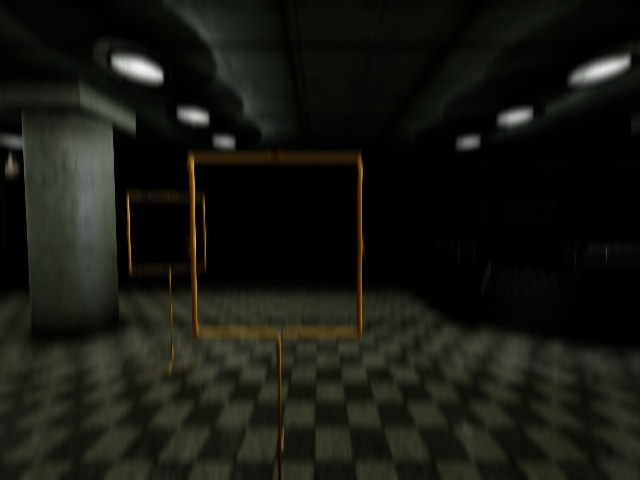
\includegraphics[width=\textwidth]{fig/gate_example_motionblur_v}
		\caption{Vertical Motion Blur.}
		\label{fig:motionblur}
	\end{minipage}
	\begin{minipage}{0.33\textwidth}
		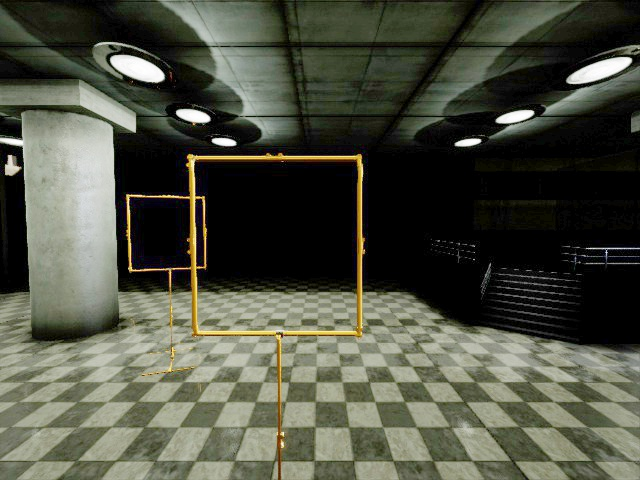
\includegraphics[width=\textwidth]{fig/gate_example_exposure}
		\caption{Exposure.}
		\label{fig:exposure}
	\end{minipage}
\end{figure}


\section{Object Detector}

This work uses a typical one-stage detector with anchor boxes as baseline, namely the \textit{YoloV3} detector with the \textit{TinyYoloV3} network. The fundamental concept of one-stage detectors with anchor boxes is illustrated in \Cref{sec:related}. In this section the implementation with the \textit{TinyYoloV3} network and its training goal are explained.

On a high level basis \textit{YoloV3} maps the input image to a predefined set of anchor boxes which are visualized in \Cref{sec:anchors}. The anchors have a predefined width $p_w$, height $p_h$ and are arranged in grids corresponding to the spatial resolution of the output layers. For objects of different scales different image features are relevant. Furthermore, for small objects a more fine grain resolution is required to sufficiently distinguish between multiple small objects close to each other. Therefore, \textit{YoloV3} uses two output grids $G=2$ output grids, with a grid of $S_1 =13$ for larger objects (red) and $S_2 = 26$ smaller objects (blue). 


For each box the network predicts an object probability $\hat o$ that classifies the class as object (1) or background (0). The original version of \textit{YoloV3} further distinguishes between object classes, however this work considers the single class case. There we remove this output node from the prediction. 

The predefined anchors only cover a subset of possible areas that can contain an object. Hence, \textit{YoloV3} also predicts how to adapt the anchor box to better fit the predicted object. These are  the bounding box center $b_x,b_y$ as well as its width $b_w$ and height $b_h$. 

In total this leads to 5 predicted parameters for each bounding box and thus to a mapping from the input image of 416x416x3 pixels to 12675 output nodes that predict 2535 boxes. In a last step boxes that contain the same class and have a high overlap are filtered such that only the boxes with the highest confidences remain.	

\subsection{Architecture}

This mapping is implemented with a \acp{CNN} as illustrated in  \Cref{fig:tinyyolov3_arch}. It contains 10 convolutional, 6 pooling and 1 unpooling layer(s). After each convolutional layer batch normalization normalizes the output in order to simplify the training process.
The input image with a resolution of 416x416x3 is processed by 5 layers that stepwise decrease the spatial resolution (max pooling) while increasing the width, leading to a intermediate volume of 26x26x512. This part can be seen as a common part that extracts features for objects at all scales. The architecture is a typical example of current \acp{CNN}. In the early layers the receptive field of the filters is small. Hence, the patterns that can be represented are not very complex and only a small amount of filters is used. As the network gets deeper more complex patterns can be present and more weights are required to encode these features. Hence, the width is increased. Research has shown that fixing kernels to a size of 3x3 and stacking them in deep layers is particularly efficient\todoref{vgg}. This can also be seen in the \textit{TinyYoloV3} architecture. 

Convolving the wide volume of deeper layers such as the 26x26x512  output of layer 5 with a 3x3 kernel requires many computations. Therefore a common technique is to first compress the volume by applying a 1x1 kernel intermediately. Such \textit{bottleneck} layers can be seen in layer 6-1 and 7-2.

From layer 5 the network splits to two branches responsible for smaller and larger objects. The lower branch extracts features for larger objects leading to a final grid of 13x13. The higher branch extracts features for smaller objects leading to a grid of 26x26. When Although not stated explicitly by the authors this is likely to compress the feature response of the previous layer and thus save computations.

In the final layer 15 output nodes are responsible to predict 3 bounding boxes for each grid cell. Thereby the nodes responsible for $\hat o$ have a sigmoid-activation such that the response gets squashed between 0 and 1 thus can be interpreted as a probability. Similarly the nodes responsible for $\hat x$ and $\hat y$ have a sigmoid activation such that the output can be interpreted as coordinate normalized to the image size. For the output nodes of $w$ and $h$ \textit{YoloV3} uses $e^x$-activation. This way the output is always larger than one while no adaption in bounding box width/height ($w=1$) corresponds to no activation. Furthermore, the network can predict a large range of scales in a small range of activation which aims to simplify the learning process.


\begin{figure}[hbtp]
	\centering
	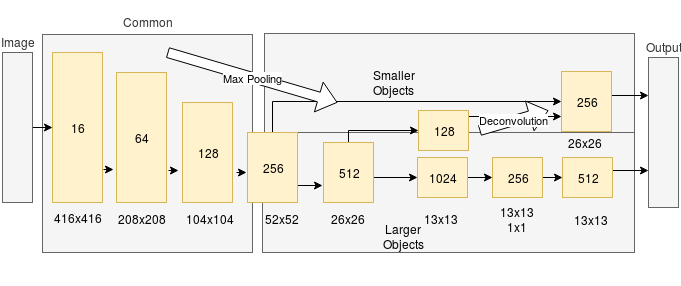
\includegraphics[width=0.8\textwidth]{fig/tinyyolov3_arch}
	\caption{The architecture of the baseline \textit{TinyYoloV3}. For each layer the amount of filters are displayed. The height of the boxes correspond to their spatial dimension. Arrows correspond to the forward pass in a network inference. In the common part the spatial resolution decreases each layer down to 26x26, while the width increases from 16 to 512. From layer 5 two branches focus on objects corresponding to different scales. }
	\label{fig:tinyyolov3_arch}
\end{figure}

	\subsection{Training Goal}

In order to train a \ac{CNN} to predict the desired properties a ground truth has to be defined for each of the 12675 output nodes. Subsequently the loss is formulated as derivable function and the \ac{CNN} can be trained with backpropagation.

Thereby it is desirable that a network output of zero corresponds to no network activation and henceforth to keep all predicted bounding boxes in the default shape. Therefore, \textit{YoloV3} encodes the ground true coordinates as follows:


\begin{equation}
\label{sec:encoding}
b_x = \sigma(\hat x_{i,j,k}) + g^x_{i,j}\quad
b_y = \sigma(\hat y_{i,j,k}) + g^y_{i,j}\quad
b_w = e^{\hat w_{i,j,k}} \cdot p^w_{i,j,k}\quad
b_h = e^{\hat h_{i,j,k}} \cdot p^h_{i,j,k}
\end{equation}

where $\hat{x}$,$\hat{y}$,$\hat w_{i,j,k}$ and $\hat h_{i,j,k}$ correspond to output nodes of anchor box at grid $i$, cell $j$, anchor $k$; $g^x_{i,j,k}$, $g^y_{i,j}$ is the top left coordinate of the respective grid cell; $\sigma$ is the sigmoid-function.

The question remains to which grid cell and anchor box a label is assigned to. Therefore the \ac{IoU} between every ground truth and anchor box is calculated and the grid with the highest value is assigned. If a ground truth box has very different coordinates than any possible anchor box, even the highest \ac{IoU} is comparatively low. Thus the network has to perform a very strong activation to predict such a label. In return the gradient will be high which can cause unstable updates. Therefore labels that have a lower \ac{IoU} than 0.5 are excluded. 

With the true label and the predicted label the training goal can be formulated. The loss needs to capture the localization and the classification goal. In a typical ground truth image only a small subset of anchors is assigned responsible to predict an object. All the other anchors see only background. Hence, there is a class imbalance between the "object" class and the "background" class. Treating both losses equally would lead the model to simply assign "background" for all anchors. The weight terms $\lambda_{obj}$ and $\lambda_{noobj}$ compensate for this class imbalance. Furthermore, $\lambda_{loc}$ trades-off the localization goal and the classification goal. The abstract training loss is summarized in: 

\begin{equation}
\mathcal{L} = \lambda_{loc}\mathcal{L}_{loc} + \lambda_{obj}\mathcal{L}_{obj} + \lambda_{noobj}\mathcal{L}_{noobj} + \lambda_{class}\mathcal{L}_{class}
\end{equation}
where $\mathcal{L}_{loc}$ is the loss for bounding box dimensions, $\mathcal{L}_{obj}$ the loss where a object is present, $\mathcal{L}_{noobj}$ the loss where there is no object. The weights are kept to the default value of $\lambda_{loc} = 5$,$\lambda_{obj} = 5$ and $\lambda_{noobj} = 0.5$.

The object loss quantifies a binary classification loss. Hence, it is the difference between a predicted probability $\hat o$ and an actual class label $c$. Where $o \in \{0,1\}$ and $\hat o \in (0,1)$. In order to learn such a goal it is desirable that the weights of the network get updated significantly when the difference between truth and prediction are high. However, when prediction and truth are already close to each other, the updates to the weights should be smaller otherwise the training might miss the optimal solution. A loss function that contains the desired properties and is used by \textit{YoloV3} is the logarithmic loss which can be formulated as follows:

\begin{equation}
\mathcal{L}_{log} = -(o_{ij}\log(\hat o_{ijk}) + (1 - o_{ij})\log(1 - \hat o_{ijk}))
\end{equation}

where $\hat o_{ij}$ is an output node with sigmoid activation assigned to anchor box $i$,$j$,$k$ and $ o_{ij}$ the ground truth label assigned to that box. The logarithmic loss is calculated for each output grid $G_i$, for each grid cell $S_j$ and each anchor box $B_k$. However, only the loss of the responsible anchor boxes are summed in the total loss calculation:

\begin{equation}
\mathcal{L}_{obj} = \sum_{i=0}^{G}\sum_{j=0}^{S_i^2}\sum_{k=0}^{B_i} \mathbb{1}_{ijk}^{obj}(-(c_{ijk}\log(\hat c_{ijk}) + (1 - c_{ijk})\log(1 - \hat c_{ijk})))
\end{equation}

Thereby the  binary variable $\mathbb{1}_{ijk}^{obj}$ is 1 if an object is present at anchor $i,j,k$. $\mathcal{L}_{obj}$ is defined vice versa but controlled by the $\mathbb{1}_{ijk}^{noobj}$ binary variable.

For the localization loss, similar to the classification loss, the weights should be updated significantly when the difference is high but less strongly when the difference is small. Furthermore, the loss should be invariant to direction. A loss that contains these properties is the squared distance between each bounding box parameter. However, the squared distance does not make a difference between large and small boxes. For example, a deviation of 5 px for a small ground truth box with a width of 1 is treated equally to a deviation from a ground truth box with width 100. Therefore \textit{YoloV3}, applies the square root on width and height to scale down very large box dimensions and thus balance the loss calculation. The localization loss is summarized in:

\begin{equation}
\mathcal{L}_{loc} = \sum_{i=0}^{G} \sum_{j=0}^{S_i^2}\sum_{k=0}^{B_i} \mathbb{1}_{ijk}^{obj}[(x_{ijk}-\hat{x}_{ijk})^2 + (y_{ijk}-\hat{y}_{ijk})^2  + (\sqrt{w_{ijk}}-\sqrt{\hat{w}_{ijk}})^2 +(\sqrt{h_{ijk}}-\sqrt{\hat{h}_{ijk}})^2 ]
\end{equation}
where $x_{ijk}$,$y_{ijk}$ are the ground truth center coordinates of anchor box $i,j,k$ and $w_{ijk}$,$h_{ijk}$ the corresponding width and height. $\hat x_{ijk}$,$\hat y_{ijk}, \hat w_{ijk}$,$\hat h_{ijk}$ are the predicted bounding box coordinates. 

The model is implemented using \textit{keras} with \textit{tensorflow} backend. 
\chapter{Experiments}

This chapter introduces the line of experiments taken out in this work and their intermediate conclusions. Initially, basic experiments about the detection of \acp{EWFO} are conducted. In further steps the insights are applied when transferring to the more challenging environment of autonomous drone races. Finally, a detector for \acp{EWFO} is deployed on an example \ac{MAV}.

\section{Experimental Setup}

The section gives an overview of the hardware used for training as well as details on the training process. Furthermore a description of particular plots used for evaluation is given.

As training a neural network is a computationally intense process common practice is to use \acp{GPU} for faster execution. In this work all trainings are carried out on a Nvidia Pascal GTX 1080 Ti GPU with 3584 cores and 11GB RAM.

The training is stopped when the performance on unseen examples does not further improve. Therefore 0.1 \% of the training samples are used as validation set. The training is stopped when the validation error converges; that is when it does not decrease for more than $1e^{-08}$ in 3 epochs.

The detector is tested by inferring the network on a given test set and calculate the metrics described in \Cref{sec:metrics}. While this gives a good estimation about the overall performance of a network it can be required to investigate the results in greater detail. It can be important to now how the detector deals with certain view points for example. In order to perform this evaluation predictions and true labels are assigned on bins based on certain conditions e.g. the bounding box size. Subsequently the performance is evaluated only for each bin individually.

In special cases it can happen that a bin border falls right between a true and a predicted label. For example a prediction is of size 10 a predicted label of size 12 and the border is at size 11. Even if the detection is correct this separation would lead to counting a missing detection as well as a false positive in each of the bins. Hence, the performance for the individual bins is typically a bit lower than when calculating a metric for the whole dataset.

The training algorithm as well as the network initialization are random processes. Hence, the network weights after training, as well as its performance are not deterministic. This condition has to be taken into account when interpreting the results. Ideally, each training is performed repeatedly and mean and standard deviation are used for evaluation. However, the training of \acp{CNN} takes a considerable amount of time which is why not all experiments can be taken out with many repetitions. Instead, trainings are performed at least two times and only further repeated if the two results have a high deviation. In plots an error bar displays the standard deviation between the different repetitions.

\section{Empty Objects}

\acp{CNN} combine simple local features to more complex patterns layer by layer. Thereby pooling removes task irrelevant information and reduces the spatial dimension. In the deeper layers features of larger areas in the image are combined and encoded in an increasing amount of filters. In the final layer each location in the volume encodes the patterns that are present in the respective field of the preceding filters and an object prediction is performed.

The power of deep \acp{CNN} arises from their capability to learn very complex patterns. However, these are not present in \acp{EWFO}. Instead most of the object area consists of background and should be ignored by the detector. We hypothesize that this emptiness makes the detection more difficult than the detection of other objects as the detector can not exploit complex patterns. Instead any object can be present within the frame and thus distract the detector.

The combination of emptiness and simple features can have further implications on the training of an Object Detector for \acp{EWFO}. If not sufficient variations in background is provided in the training set, a detector is likely to overfit to the background of the training set. This condition can be amplified for more complex architectures with more parameters.

To summarize our hypotheses are:
\begin{enumerate}
	\item Compared to a simple filled object, the detection of \acp{EWFO} is harder, as the object does not provide complex patterns and a detector can be confused by patterns that are present in the empty part. 
	\item Compared to a complex filled object, the detection of \acp{EWFO} can not be improved by using a deeper network.
	\item Compared to other objects \acp{EWFO} do depend more on background. If the environment in the training set is different to the test set, the performance drop for \acp{EWFO} is higher than for other objects. 
\end{enumerate}

In order to evaluate these hypotheses the detection of an \ac{EWFO} is compared to a comparable object where the empty part is filled with a certain pattern. The created objects \textit{Cats} and \textit{Sign} are visualized in \Cref{fig:cats}. Thereby a simple object is chosen such as the stop sign which is clearly distinguishable from the background. This is compared to a more complex object such as the cat image.

The created objects allow to study how a detector performs that is trained on a filled object. Also, it allows to study how the detector for \acp{EWFO} reacts when during testing another pattern is present in the empty part.

\begin{figure}[hbtp]
	\centering
	\begin{minipage}{0.3\textwidth}
		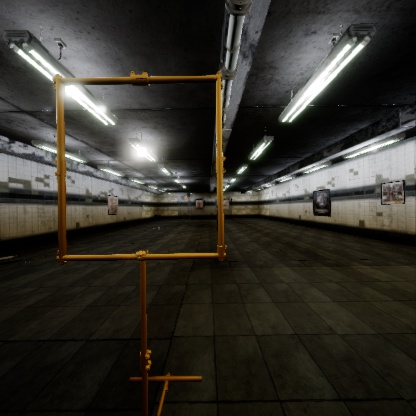
\includegraphics[width=\textwidth]{fig/gate}
	\end{minipage}
	\begin{minipage}{0.3\textwidth}
		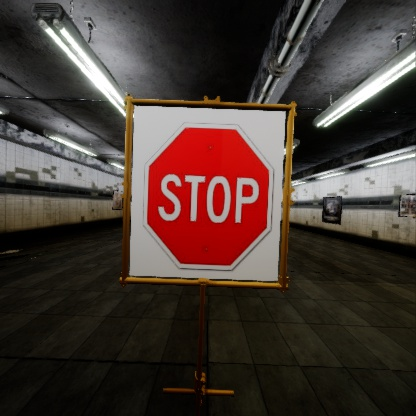
\includegraphics[width=\textwidth]{fig/sign}
	\end{minipage}
	\begin{minipage}{0.3\textwidth}
		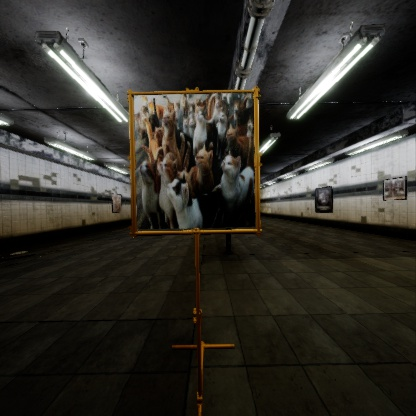
\includegraphics[width=\textwidth]{fig/cats}
	\end{minipage}
	\caption{Examples of the three objects that are compared. The \acp{EWFO} object (\textit{Gate}) left is compared to a simple solid object (\textit{Sign}) in the center and a complex solid object on the right (\textit{Cats}).}
	\label{fig:cats}
\end{figure}

\subsection{Training Set}

For each object a dataset with 20 000 samples is created within the \textit{Dark} environment. As this experiment focuses on the influence of the empty part of the object, the view points are limited to frontally facing the object in various distances. On these training sets the two architectures illustrated in \Cref{sec:meth} \textit{SmallYoloV3} and \textit{VGGYoloV3} are trained. As 20 000 samples is a comparatively small amount of samples for a network such as the \textit{VGGYoloV3}, the network is initialized with the weights of the \textit{VGG-19} pretrained on ImageNet.


\subsection{Test Set}

For each object a test set of 200 samples is created within the \textit{Dark}-Environment, as well as the \textit{IROS}-Environment. Hence, in total there are 6 test sets with 150 samples each. Similar to the training set the view points are limited to frontally facing the object at various distances.



\subsection{Results}

\begin{table}
	\centering
	\input{tables/all_basement.txt}
	\caption{Performance of two architectures when the test environment is similar to the training environment. Each trained network (row) is evaluated on each test set (column). It can be seen how the detectors exploit the structure that is placed in the object. In contrary, the detector of \acp{EWFO} only gets confused when the structure inside the object is very different from the training set.}
	\label{tab:all_basement}
\end{table}

\Cref{tab:all_basement} shows the results in the \textit{Dark}-environment. It can be seen how the best results are obtained for the \textit{Cats}-object. Yet when the structure is removed the performance drops almost to zero. A similar observation can be made for the \textit{Sign}-object. In both cases the performance can not really be improved by using a deeper network.

For detecting the \textit{Gate}-object, the lowest performance is achieved. When the same detector is applied on an object where the empty part is filled, the performance drops. This happens particularly for the \textit{Sign}-structure. For the \textit{Cat}-structure the performance drop is lower. In fact for the deep network there is not really a performance drop measurable.

\begin{table}
	\centering
	\input{tables/diff_iros.txt}
	\caption{Change in performance when the detectors are tested in another environment than their training environment. The most severe drop can be seen at the \textit{Cats}-object. The drop for \acp{EWFO} is comparable to the \textit{Sign}-object}
	\label{tab:diff_iros}
\end{table}

\Cref{tab:diff_iros} shows the change in performance when the trained detectors are applied in a different environment. All detectors are subject to a significant drop, however the strongest effect can be seen for the \textit{Cats}-object. While the \textit{Sign}-object can still be detected best, its relative performance drop is comparable to the \textit{Gate}-object. The network size does not have a significant effect when changing the test environment.

\subsection{Discussion}

It can be seen how the detector exploits the added structure in the filled objects. The performance is much better than for the \textit{Gate} object. Also, when the detectors trained with added structure are applied on the empty object the performance drops. Thereby the network size is of minor effect. No performance boost is achieved even for the more complex \textit{Cats} object.

When the test environment changes, the most complex object can almost not be detected anymore. It seems that the detector particularly overfitted to lightning conditions and background. This is surprising as the background in the \textit{IROS}-environment is lighter and thus the object is better visible than in the \textit{Dark}-environment.

The simple but solid object is subject to a smaller performance drop when the environment changes. In the new environment it can still be detected best. This is likely because the surface mainly consists of a white and red area which gives distinctive shape and colour.

The detector for the \textit{Gate}-object is less subjective to changes in the empty part as expected. When applying the detector on objects with the \textit{Cats} structure some performance can still be reached. The deep architecture does not suffer any performance drop in this case. This is likely because the \textit{Cat} structure is of similar shape and colour as the background. When adding a very different structure such as the \textit{Sign} object, the performance drops almost to zero.

The background dependency is also lower as expected. When moving to a new environment the performance drop is not higher than for the other objects.


\subsection{Conclusion}

In this section we compared the \ac{EWFO} investigated in this work to objects of similar shape that contain a structure inside the empty part. We hypothesized that a \ac{EWFO} is harder to detect as it provides less features the detector can use. This hypothesis can be confirmed as when adding structure inside the empty part the performance gest significantly better. 

Furthermore, we hypothesized that due to the empty part a detector for \acp{EWFO} is more dependent on the training environment than for other objects. However, this hypothesis could not be confirmed. The performance drop for other objects is at least equally high. 

Also, we hypothesized that in contrast to a more complex object the detection of \acp{EWFO} can not be improved by using a deeper network. While this could be confirmed for the \ac{EWFO}, in the experiments there is neither an improvement for the other objects. Yet it can be seen how the deeper network is less confused when adding the \textit{Cat} structure.

\section{Providing Background}

In the previous experiments it could be seen how the performance of a detector drops significantly when applying it in an environment that is different to the training environment. In this section it is investigated how to make the the detector less dependent on such domain shifts.

A simple method is to create more data by placing the object in front of backgrounds of different images. This way the detector can learn to be background invariant. However, with this placement the object is not aligned with its context anymore. The light conditions do not fit to the remaining image and also perspective properties are violated that otherwise could be exploited by the detector. Another method is to create new environments in simulation and change light conditions and background there. This requires more manual work but leads to geometrically aligned images. Yet, the images consist only of synthetic elements.

We hypothesize that the creation of samples with a simulator leads to better results than when simply replacing the background. Therefore a detector is trained with both methods. The detectors are evaluated on the test sets created in the previous section.

\begin{figure}[hbtp]
	\centering
	\begin{minipage}{0.3\textwidth}
		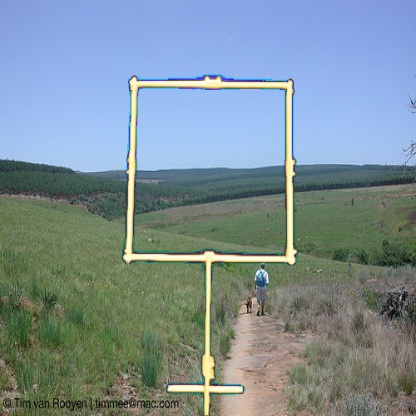
\includegraphics[width=\textwidth]{fig/voc}
	\end{minipage}
	\begin{minipage}{0.3\textwidth}
		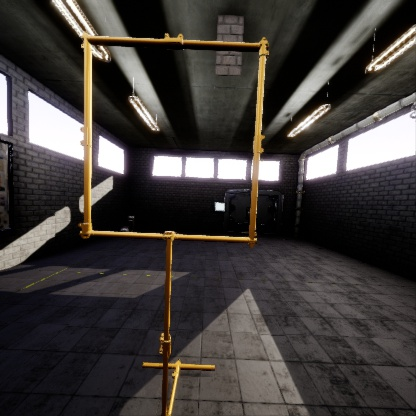
\includegraphics[width=\textwidth]{fig/sim}
	\end{minipage}
	\caption{Examples of samples with more background. On the left a sample augmented with an image from the Pascal VOC 2012 dataset. On the right a sample generated in the \textit{Daylight} Environment. Although on the left the background contains realistic data the scene does not align with the objects. Also the shadows to not fall correctly. With the simulated environment the general scene looks more realistic although the background is synthetic.}
	\label{fig:sim_vs_voc}
\end{figure}

\subsection{Training Set}

With both methods a dataset with 20 000 samples is created. The view points are limited to frontal views.

The simulated dataset is created using \textit{Daylight} and \textit{Dark} environment which have different lightning conditions. Additionally, the backgrounds in both environments are varied such that a higher variance in background textures is achieved. Thereby the background texture that is present in the \textit{IROS} environment is not used.

For the dataset with random backgrounds 2000 view points are created in a black environment. Subsequently the black image part is replaced with a randomly selected image from the Pascal VOC dataset \todoref{voc}.

\subsection{Results}

\begin{table}
	\centering
	\input{tables/sim_vs_voc.txt}
	\caption{Performance of \textit{SmallYoloV3} in the \textit{IROS} environment when adding more variance in the background. It can be seen how including more backgrounds improves the results especially when the environment is fully simulated. Furthermore, the detector has learned to be more invariant structures that are present inside the image.}
	\label{tab:sim_vs_voc}
\end{table}

\Cref{tab:sim_vs_voc} shows the results. Selecting the backgrounds randomly thereby only led to a minor improvement. In contrast, simulating more environments and backgrounds improved the performance by 50\%.

For both methods the detectors became less subjective to patterns present in the empty part. The detector trained on simulated images achieves equal performance when there is a \textit{Cat} structure present. Also, the performance drop for the \textit{Sign} structure is less severe. Interestingly, the detector trained with random backgrounds even detects more gates when there is a \textit{Sign} structure present in the empty part.

Another observation is the higher variance in the results. Especially, when trained with random backgrounds the standard deviation is quite high. \todo{double check this with another iteration}


\subsection{Discussion}

Providing more samples from different environments was crucial for better performance. The results are even better than the ones achieved when the detector was trained and tested in the \textit{Dark} environment (\Cref{tab:all_basement}). By supplying more backgrounds the detector could learn an overall better representation. However, it seems similarly crucial to provide realistic environments. The detector trained on random backgrounds only achieved minor improvement.

Providing more variation in background also helped the detector to ignore the background. The performance drop when placing patterns inside the object is smaller.

\subsection{Conclusion}

In this section we investigated how to make the detector more invariant against changes in background and the environment. By increasing the training set with samples in front of different backgrounds this was achieved. This method even improved the results beyond its previous highest score. Thereby it seems important to provide a realistic alignment of object and scene. When simply pasting the object on random images only minor improvements could be achieved.

\section{Transferring the detector to an \ac{MAV} race}

Until now the conducted experiments where limited to relatively simple environments. In a real world application such as an \acp{MAV} race, much more objects are in sight. These can not only appear frontally but also in more difficult view angle. Furthermore, the objects can appear behind each other, such that in the empty part, another object is visible. This section studies whether the results obtained so far also apply in a more challenging environment. Therefore different architectures and training methods are evaluated on the synthetic test set described in \Cref{sec:datasets}.

Due to the challenges in this dataset we hypothesize that the detector trained so far will perform poorly on this dataset. In order to handle overlapping objects in difficult angles, such situations should be included in the training set. Yet, the amount of possible views/overlaps is large and manually constructing such examples is cumbersome especially considering the amount of samples required to train a \acp{CNN}. A simpler way is creating a scene with several objects and placing the camera randomly (within some margin) in order to cover a large variation of views on the scene. That way the network should learn a general object representation and detect unseen objects from different view points. However, this \textit{Random Placement} might not resemble the real world sufficiently. An \ac{MAV} does not appear at random places within a scene, especially not when it follows a racing track. Alternatively, the samples can be generated by simulating a flight through a race court. Although such a \textit{Simulated Flight} requires to create a race court an a corresponding trajectory the obtained samples should resemble the real world better. 

In order to examine this further the view points of random placement and a simulated flight are compared. Therefore, 600 samples are created using random placement with the following distributions:

\begin{equation}
x = \mathcal{U}(-30,30),\quad y = \mathcal{U}(-20,20),\quad z = \mathcal{N}(-4.5,0.5)),\quad
\phi = \mathcal{U}(0,0.1\pi),\quad \theta = \mathcal{U}(0,0.1\pi),\quad \psi = \mathcal{U}(-\pi,\pi)
\label{eq:distroexp}
\end{equation}
Where $\mathcal{U}(a,b)$ is a uniform distribution with borders $a$ and $b$; $\mathcal{N}(\mu,\sigma)$ a Gaussian distribution with mean $\mu$ and variance $\sigma$. The labels are compared to the ones from the synthetic dataset described in \Cref{sec:datasets}.

\begin{figure}
	\begin{minipage}{\textwidth}
		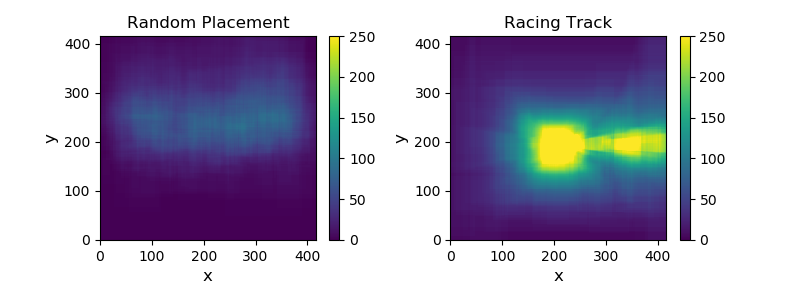
\includegraphics[width=\textwidth]{fig/heatmap_camplace}
		\caption{Object appearances in 2D when generating samples with random poses (left) and during a \ac{MAV} flight. Each pixel value corresponds to the number of labels that cover this particular pixel. In the simulated flight objects appear mostly centred on the horizontal line.}
		\label{fig:heatmap_camplace}
	\end{minipage}
	\begin{minipage}{\textwidth}
		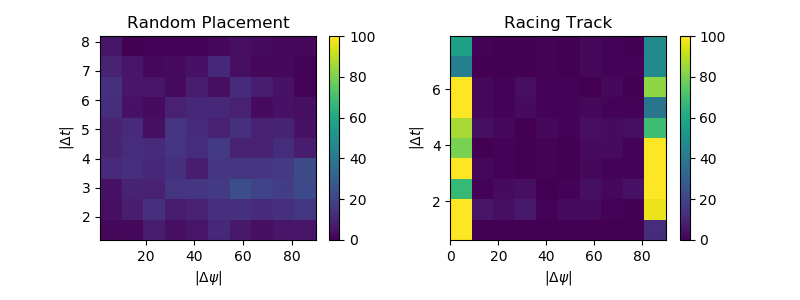
\includegraphics[width=\textwidth]{fig/hist2d_camplace}
		\caption{Histogram of object occurrences in $\Delta \psi$ and euclidean distance relative to the camera.$\Delta \psi = |\delta t| = 0$ corresponds to flying through the centre part. With a $\Delta \psi = 90\degree$ the object appears as straight line for $\Delta e = 0$. For $\Delta e > 0$ and $\delta \psi = 90\degree$ the object can be seen as squeezed quadrangle. It can be seen how the random placement does rarely cover facing the object closely and frontally. }
		\label{fig:hist2d_camplace}
	\end{minipage}
\end{figure}

\Cref{fig:heatmap_camplace} shows the distribution of bounding boxes when created with random camera placement and when following a racing track. Thereby each pixel value corresponds to the number of labels that cover this particular pixel. It can be seen how, when following the race track most of the objects are centred and distributed across the horizon, as camera focuses the next object frontally most of the time. In contrast, random placement leads to more evenly distributed object locations. 

This can also be seen in \Cref{fig:hist2d_camplace} where a 2D histogram of the $\Delta \psi$ and $|\Delta t|$ with respect to the camera is displayed. Thereby a $\Delta \psi = |\Delta t| = 0$ corresponds to flying through the centre part. For $\Delta e = 0$ and $\Delta \psi = 90\degree$ the object appears as straight line. For $\Delta e > 0$ and $\Delta \psi = 90\degree$ the object can be seen as squeezed quadrangle. It is apparent how the random placement covers a much larger range of relative angles, while in the racing track certain angles do not appear at all. Even more importantly the largest bins of the racing track is an angle of 0 and a distance between 0m and 4m. These bins are almost not present when placing the camera randomly. This is because close to the camera the field of view is small, while the area of the object faced frontally is big. Hence, the probability of an object ending up at this specific location is relatively low. Furthermore, when placing the camera randomly there are no samples further away than 8m. This is because in the race track the camera traverses the room from one end - where it can see almost all gates - to another. The probability that the randomly placed camera ends up in a similar position is relatively low.

We hypothesize that there is a trade-o
Although \textit{Random Placement} covers more and better distributed view angles, it misses certain object appearances that are typical in a \ac{MAV} racing. On the other hand, when simulating a flight the samples strongly depend on the racing track as well as the trajectory the camera flies. We hypothesize that there is a trade-off between generalizability and specialization. A detector that has to cover more view points will have a larger recall but be less precise in its predictions. 


\subsection{Training Set}

Training sets with 20 000 samples each are created using \textit{Random Placement} and \textit{Simulated Flight} in each of the environments described in \Cref{sec:meth}. In each environment the background textures are varied during data generation. For \textit{Random Placement} the gates are placed throughout the room, subsequently the camera is placed according to \Cref{eq:distroexp}. For \textit{Simulated Flight} 3 race courts with corresponding trajectories are created. It should be noted that the race court present in the test set is not part in either of the training sets.

\begin{figure}
	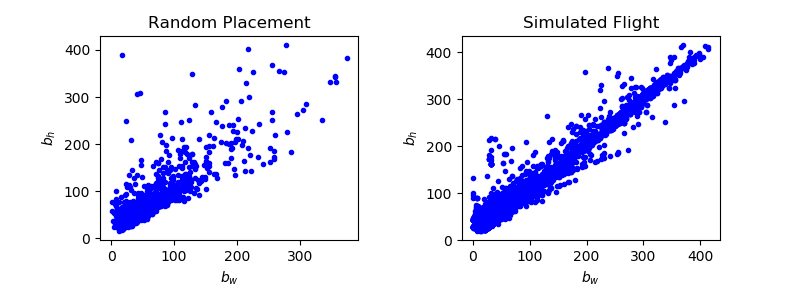
\includegraphics[width=\textwidth]{fig/ar_train}
\end{figure}

\subsection{Results}

The results are presented in \Cref{fig:view_size}. Predicted and true labels are assigned to bins based on their covered area $A_O=b_w*b_h$. Subsequently $ap_{60}$ is evaluated for each bin. 

\begin{figure}
	\centering
	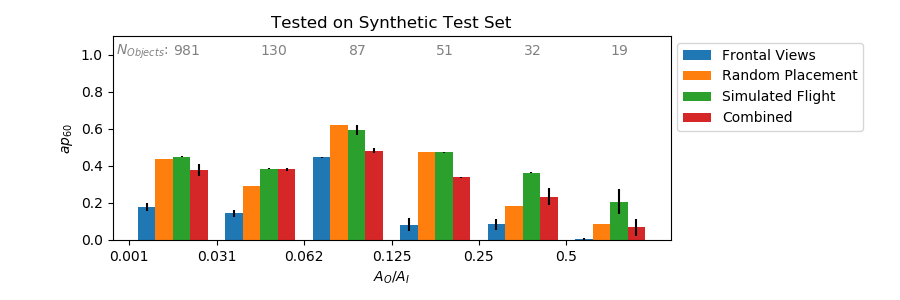
\includegraphics[width=\textwidth]{fig/view_size}
	\caption{Results of different methods to include more samples in the training set. The results are clustered based on the size of the true/predicted bounding box. It can be seen how the network that contained only frontal views performs poorly when applied in the simulated \ac{MAV} race track. The network trained with images obtained with \textit{Simulated Flight} outperforms the network trained on samples obtained with \textit{Random Placement} for larger object sizes.}
	\label{fig:view_size}
\end{figure}

\textit{Frontal Views} is the network trained in the previous section. Its training set contained only frontal views and no overlap. It can be seen how it performs poorly when simulating a whole \ac{MAV} race. \textit{Random Placement} achieves competitive performance for smaller object sizes until 25\% of the input image. However, the performance drops below 20\% for larger objects. \textit{Simulated Flight} achieves competitive performance on all bins. Only for objects of a size between 6.2\% - 12.5\% of the input image the random placement performs slightly better. 

Overall a significant drop in performance can be seen compared to the test sets of the previous sections. Only on the bin for objects of a size between 6.2\% - 12.5\% of the input image the networks achieve a comparable performance of 69 \%. This bin seems to be the optimal distance for all networks. Especially for larger objects the performance decreases.

\subsection{Discussion}

In the results it can be seen how the detectors struggle in the more challenging environment of a \ac{MAV} race. A drop in performance can be seen for all detectors. Including new view points in the training set helped counteracting against this drop. The networks trained with more view points perform significantly better than the network which was only trained on frontal views.

The question remains what view points to include. The capability of the detector to generalize across view points seems quite poor. Despite the fact that \textit{Random Placement} contains close up views on the object, it performs poorly for larger objects. In contrary \textit{Simulating Flight} works much better on this data set. However, its data generation assumes a certain motion model of the camera as well as certain patterns in race courts.

Overall we see a performance drop for larger objects. We assume the reasons that less context is visible, also the features are spread more apart.

\subsection{Conclusion}

In this section we evaluated how the detector performs when applied in \ac{MAV} racing. It can be seen how such an environment is more challenging for the detector. Incorporating the pattern of a \ac{MAV} race improved the performance.

\section{Transferring the detector to the real world}

After having investigated the performance of the detector in challenging environment such as an \acp{MAV} race, it is time to perform experiments on real data. This section investigates the reality gap and several methods to reduce it.

In literature \cite{Krizhevsky2012a,Howard2013,Redmon,Liu} the application of image augmentation is a common tool to improve the detection performance. The experiments in \cite{Carlson2018} show how the incorporation of sensor effects particularly improves the performance of models learned on fully synthesized data. In the \ac{MAV} domain sensor and lens effects have a significant influence on the obtained sample. Hence, we hypothesize that the incorporation of these effects will improve the performance of the detector. A total of  five image augmentation techniques are investigated.

\subsection{Results}

\begin{figure}[htbp]
	\centering
	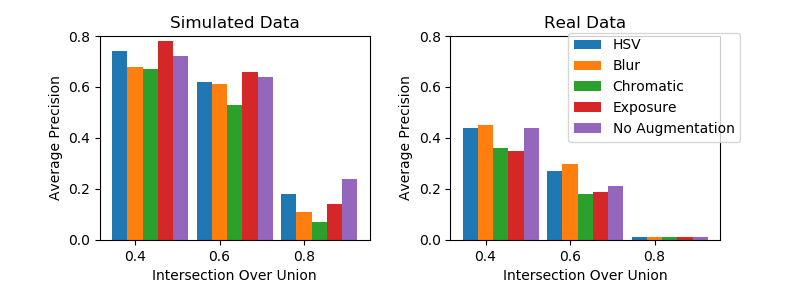
\includegraphics[width=\textwidth]{fig/pp_bar}
	\caption{Performance in terms of Average Precision for different methods  of image augmentation.}
	\label{fig:pp_bar}
\end{figure}

\Cref{fig:pp_bar} shows the results in terms of average precision in the training domain. On the simulated data variations in exposure improve the performance of low quality predictions slightly compared to using no augmentation. However, using no data augmentation achieves the best performance for high quality detections. The other effects have only minor influence. 

On the real data variations in HSV space as well as blurring improves the results compared to not using data augmentation. Incorporating chromatic aberration and variations in exposure lead to a deterioration in performance.

\subsection{Discussion}

In simulation the data augmentation has only a minor effect on low quality predictions, while the performance in high quality predictions decreases. As most effects are not really present in the test set this confirms that the models can learn a robust representation. Despite having more noise in the training data, the performance on the test set stays the same. However, the added noise leads to a lower quality in the predicted bounding boxes.

On the real data there is a stronger effect measurable. Variation in HSV and image blurring increase the performance compare to not using data augmentation. This meets our hypothesis that variations in HSV help to achieve a model that is more robust against changes in colour. Blur is one effect that can clearly be seen in the real world test set. Including this effect in the training process helped the model to perform better in the real world. Chromatic Aberration led to a significant improvement in \cite{Carlson2018} however, we cannot confirm these results. It is possible that our camera suffers only little from  chromatic aberration and thus including the effect in the training does not further help the prediction. The same holds for variations in exposure. 

\subsection{Conclusion}

We investigated whether including sensor effects present in the target domain in the data generation process can improve the detection. Therefore we modelled several effects that were observed when working with the camera or that improved the detection in experiments conducted in literature. Finally, image blurring improved the detection. Other effects led to a deterioration in performance.

We also investigated image augmentation by adding variations in HSV-space to evaluated whether this improves the robustness of the model, improving the performance on the real world dataset. We can confirm this hypothesis and conclude that this image augmentation should be part of the training process.


\section{Deploying the detector on a \ac{MAV}}

In the application of the detection of \acp{EWFO} on a \acp{MAV} detection accuracy is only one important metric. Equally relevant are inference speed and energy requirements. The example control loop in which the detector of this work is integrated, contains a filtering stage which fuses measurements of different sensors over time to infer a global state. This stage can deal with outliers and henceforth it can be more important ot have more bad detections in high frequency than only slow but good ones. This section studies the deployment of a detector for \acp{EWFO} on a \ac{MAV} in the example of the target system of this work. Therefore the performance-accuracy trade-off is studied and an experiment in a real world flight is conducted.

As explained in \Cref{sec:background} the execution time strongly depends on the used hardware as well as its low level implementation. Therefore the inference time of several layers is measured on the JeVois using the \textit{Darknet} framework. The results are displayed in \Cref{fig:bottleneck_jevois}. Each sample corresponds to the number of computations and their computational time in one layer. Dashed lines connect samples at the same resolution. It is apparent how the same amount of computations at a spatial resolution of 20x15 is more than 4 times faster than at a resolution of 160x120. We assume this is because parallelism is better exploited at the lower scale.

\begin{figure}[hbtp]
	\centering
	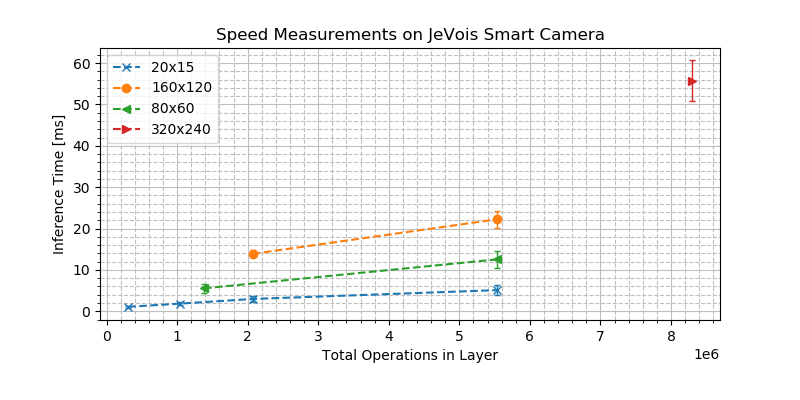
\includegraphics[width=0.8\textwidth]{fig/bottleneck_jevois}
	\caption{Inference Time of different layers on the JeVois. Each sample corresponds to the inference in a single layer. Dashed lines connect samples at the same resolution. It can be seen how an operation at a higher spatial resolution is significantly slower.}
	\label{fig:bottleneck_jevois}
\end{figure}


\textit{TinyYoloV3} is optimized to detect solid feature rich objects of multiple classes with a low computational budget. In order to sufficiently represent and distinguish such objects many weights are required. Hence, the network contains 9 layers and a final width of 1024. In contrast, the features of \acp{EWFO} are relatively simple hence less weights should be required. Therefore we hypothesize a thinner network should be able to learn the task equally well while being computationally more efficient.

The receptive field of \textit{TinyYoloV3} is 223 pixels which does not cover the full input image. For solid objects this is of minor impact as even if the network only sees an object part it can still learn to recognize it. However, this does not apply for \acp{EWFO} which are empty and do not contain any information in the object centre. Instead it can confuse an output layer that is assigned responsible to detect such an object. Therefore we hypothesize that more layers should improve the performance for larger objects. However, the c 

Yet, the complexity of large objects does not increase. Hence, we hypothesize that if the receptive field is large enough,  performance for larger objects. 

Another parameter are network width and depth.  The same condition holds for the number of layers. However, more layers also increase the receptive field. Hence, we expect the performance to increase as long as the receptive field does not fully capture the image.

In order to evaluate our hypothesis we perform an architecture evaluation by varying the number of layers filters and the receptive field. Before training the networks we tune the anchor box dimensions by performing a k-means clustering on t

Initially an architecture evaluation is performed. Therefore different architectures are trained and evaluated in terms of \ac{ap60}. As an architecture contains many parameters we can not simply vary each of them independently. Hence, three experiments are performed iteratively. We first describe them on a high level basis before explaining the exact changes. In a first step the width is decreased until a drop in performance is noticeable. In a second step the architecture with the lowest width but without performance drop is chosen and the depth is varied. Based on the results of this step we create a final model that combines the gained insights and tune the anchor boxes.

The scheme in which the architecture is changed is visualized in \Cref{fig:depth_changes}. The width of the baseline model is decreased stepwise by a factor of two. When decreasing depth only convolutional layers are removed while the pooling layers are kept such that the spatial resolution stays the same. When increasing depth 2 layers are inserted stepwise at the end of both branches. The results show how depth is mainly relevant to detect objects of larger scale. Hence, the final model consist of 5 common layers, 15 layers on the branch to detect larger objects and 2 layers on the branch to detect small objects.


This means most speed can be gained when reducing the number of computations in the early layers where the spatial resolution is high. In earlier experiments it could be seen that already a small amount of filters is enough to detect \acp{EWFO}. However, even evaluating 4 kernels at a resolution of 320x240 already takes 55 ms (\Cref{fig:bottleneck_jevois} red triangle). A total network of that size would require more than 200 ms and is thus too slow to be deployed in the control loop.

Current research mostly addresses to reduce the computations when the convolved volumes are deep or the operations are performed on \acp{CPU} that do not support floating point operations. However, the bottleneck on the JeVois happens at shallow volumes and the hardware can perform floating point operations. Furthermore, \acp{EWFO} consist of thin elements that are spread over large parts of the image. Hence, we hypothesize that simply reducing the image resolution will lead to large drops in performance. An alternative is to increase the stride parameter in the early layers of the network. This reduces the number of locations at which the kernel is evaluated. \acp{EWFO} are sparse and spread over large parts of the image, while most of the image does not contain useful information. Hence, we hypothesize that increasing the stride parameter in the early layers will perform better than reducing the image resolution.

\section{Experiments}

In order to answer this question we measure the inference time of different model architectures. This enables us to investigate the bottlenecks and thus optimize the model architecture. The JeVois Smart Camera uses an aspect ratio of 4:3. Therefore we change the network resolution accordingly. The JeVois Smart Camera has only limited memory available. Using a network architecture that goes beyond the memory simply results in a system crash. For example our baseline network runs performs one network evaluation in 700 ms. This is at a resolution of 160x120.

In order to evaluate our hypotheses the network is trained with different architectures. Subsequently, performance and inference time on the JeVois are measured.

The JeVois supports aspect ratios of 4:3 and resolutions of 160x120, 320x240 and 640x480. Although, \ac{FCN} do not depend on the image resolution, the object appearance can change at lower image resolution. Hence, during training the images are scaled to 160x160 or 320x320 respectively. The anchor boxes are scaled in similar fashion. Finally, as the input image resolution decreases, the output grid size decreases by the same factor. This is not desirable as the output resolution should stay the same. Hence, when decreasing the input image to 160x160 we remove the last pooling layer such that the output grid stays at 20,20 or 10,10 respectively.

\section{Results}

\begin{figure}[hbtp]
	\centering
	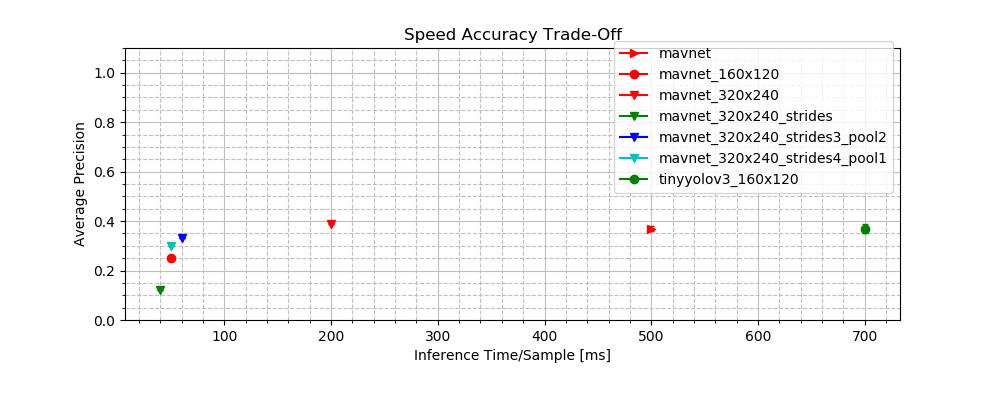
\includegraphics[width=0.8\textwidth]{fig/ap_speed_tradeoff}
	\caption{Inference Time of different layers on the JeVois. Each sample corresponds to a single layer. On the x-axis the total number of multiplications in that layer is displayed. It can be seen how an operation at a higher spatial resolution is significantly slower.}
	\label{fig:ap_speed_tradeoff}
\end{figure}

Due to their computational complexity deploying a \acp{CNN} on mobile devices is a challenging task


\Cref{fig:perf_width} shows the performance for thinner and wider networks. It is apparent how the performance only undergoes slight variations despite reducing the total number of weights by a factor 1000. \todo{retrain one in the middle to get variance, it should be more linear}


\begin{figure}[hbtp]
	\centering
	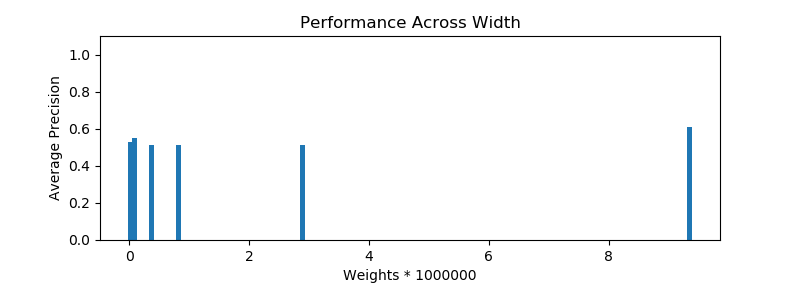
\includegraphics[width=\textwidth]{fig/perf_width}
	\caption{Performance in simulation when varying the amount of filters per layer. Starting from the baseline architecture with approximately 9 Mio. weights, the amount of filters per layer are decreased stepwise by a factor of 2. Only minor effects on performance can be seen, despite reducing the flexibility of the model.}
	\label{fig:perf_width}
\end{figure}

\begin{figure}[hbtp]
	\centering
	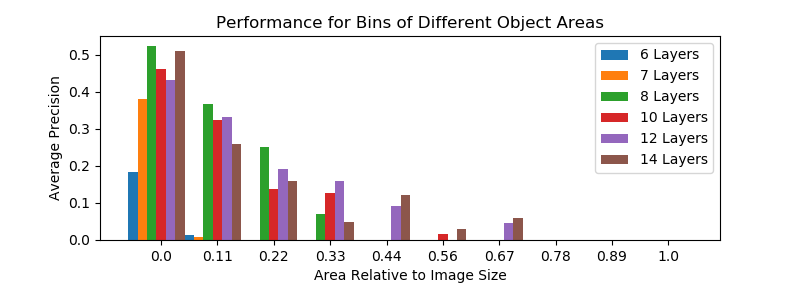
\includegraphics[width=\textwidth]{fig/depth_ap_size}
	\caption{Performance in simulation of models with varying depth and for bins of different size. It can be seen that the performance for larger objects increases with the amount of layers.}
	\label{fig:depth_ap_size}
\end{figure}

\Cref{fig:size_bins} shows the distribution of object sizes in the bins used for evaluation. It can be seen that most objects in the test set are further away. \todo{put some examples to show what each size actuall means}

\begin{figure}[hbtp]
	\centering
	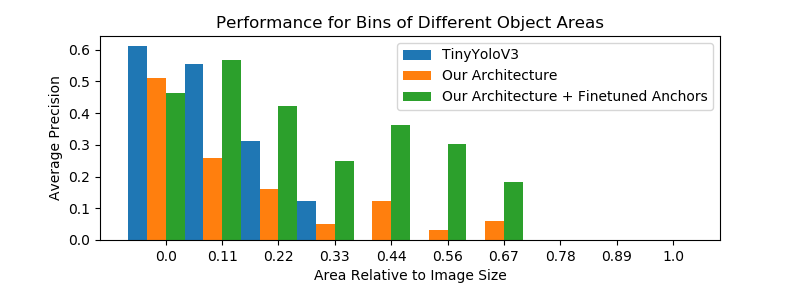
\includegraphics[width=0.8\textwidth]{fig/hyperparam_size}
	\caption{Architectural Changes when varying the depth. The upper graph shows in which order layers are removed. The lower graph shows how layers are added. Depth is increased by inserting two layers on each branch (green). }
	\label{fig:hyp}
\end{figure}

\begin{figure}[hbtp]
	\centering
	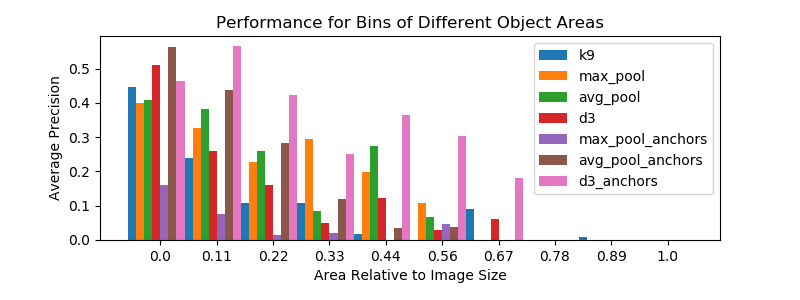
\includegraphics[width=\textwidth]{fig/rf_ap_size}
	\caption{Label distribution in bins of different object size. As the field of view is larger for objects further away, the proportion of small objects is higher.}
	\label{fig:size_bins}
\end{figure}

\subsection{Discussion}

The overall performance is only slightly affected when reducing the number of weights in terms of width and height. We can assume that this is because the objects we investigate are of quite simple structure. Intuitively the features to be considered are color, lines and edges in certain combinations. Hence, it seems logical that only a few filters are necessary to represent these shapes.

The performance in terms of different object sizes varies significantly for models with varying depth. Only deeper networks are able to detect larger objects. However, the complexity of the object does not increase for closer objects. In contrary the closer the objects are, the less context is visible. A very close object consists "only" of an orange square. Hence, it is unlikely that increased flexibility is the reason for the increase in performance. 

Instead it is more likely that the increased receptive field is the reason for the improved performance. In fact only the network with 14 layers has a receptive field of 414 an thus covers the whole image. Yet even this network cannot detect the largest objects. Thus the receptive field can not be the only reason for the lower performance on larger objects.

The current structure combines features distributed across space in a pyramid fashion. So 3-by-3 convolutions are performed layer by layer such until the whole image is covered. For \acp{EWFO} many of these steps are unnecessary as the objects are empty and the network should learn to ignore the empty part in the centre. It is possible that this structure gets confused by the parts that are present in the image centre.

\subsection{Conclusion}

We investigated how width affects the performance for the detection of \acp{EWFO}. We hypothesized that due to the low variance in the investigated object and the simple features, less filters are required than in the baseline architecture. We can confirm this hypothesis as we see that the width can be decreased by a factor of 10 without loosing performance. This leads to a reduction of weights by a factor of 1000. 

Furthermore, we investigated how depth affects the performance of the model. We hypothesized that a shallow network should be able to detect the object as it only consists of relatively simple features. We can see how depth is required in order to cover the whole input image. Hence, we cannot fully conclude whether depth is required for the increased flexibility or simply due to the receptive field. 






%\chapter{Transfer Learning}
\label{sec:training}

Supervised machine learning relies on the assumption that a hypothesis $h$ can be learned from a limited set of samples $X$ with their corresponding set of labels $Y$. The goal is to learn $h$ from a source set $D_s = \{X_{s},Y_{s}\}$ such that it can be applied on a target set of unknown examples $D_t = \{X_{t}\}$ to obtain the corresponding labels:

$$
h(X_t)\rightarrow Y_t
$$ 

Whether $h$ is performing well, can evaluated by splitting the labeled set of $D_s$ in a training set $D_{train}$ and test set $D_{test}$. $h$ is learned using the full information of $D_{train}$ and applied on the $D_{test}$. By evaluating a performance metric $m_A$ on $D_{train}$ information about the representation strength of $h$ can be inferred. The performance metric $m$ on $D_{test}$ gives an estimate of the performance of $h$ on $D_t$. Comparing $m_A$ and $m$ allows to evaluate whether model and dataset are suitable for the task.
			
This basic supervised machine learning setting relies on the assumption that $D_s$ follows the same i.i.d distribution as $D_t$. However, this can not be assumed for the application of this thesis. As most of the data is artificially created it will share properties with the real data but only to the extent that they can be modeled during creation. For example a graphic engine can not fully capture visual properties of all materials and light sources. Furthermore, is this model developed for application in locations with unknown light conditions and object variances that can be significantly different to the ones used at training time. When the source domain $S$ only shares a subset of properties with the target domain $T$ this is also referred to as a domain shift scenario. 


Learning models in such an environment is concerned by the field of Transfer Learning. The goal is to find a concept $h$ that performs best in the target domain $T$. Similar to $m_A$ and $m$ the performance $m_s$ in $S$ and the performance $m_t$ in $T$ can be used to evaluate whether a suitable model/dataset has been chosen/is available.

The task of learning from synthetic data can be summarized in:

$$
\text{arg}\max\limits_{h,S} m_t
$$

The goal is to create source domain $D_s$ and find a concept $h$ that maximizes its performance in the target domain $m_t$. This formulation yields two levels at which the domain shift problem can be addressed: (1) focusing on generating data or (2) focusing on finding a hypothesis that maximizes the performance.

In this thesis two types of domain shifts are considered: (1) A semi-supervised domain shift between synthetic data and real images. This means $D_s$ is available in large quantity, namely it is generated by a graphical engine. For $D_t$ a considerably smaller amount of labels is available \todo{describe real datasets}. 
(2) An unsupervised domain shift when environment conditions at test time can be significantly different to the ones at training time. In this case information about $D_t$ is only available as graphical models of the object of interest and several images of the domain. \todo{double check is this really an unsupervised domain shift since we dont even know X}

The conducted research is limited to \ac{CNN}-based object detection as they are investigated in this thesis. The chapter focuses on domain adaption while the exact model is described in \autoref{sec:object_detection}.

The relevant question to be investigated in this chapter is the following:

\begin{center}
	\textbf{How can data be generated to train a model for wire frame object detection?}
	\textbf{How can the model be made robust against domain shifts?}
\end{center}

The first question will be answered by choosing a state of the art method for object detection and training it with varying properties in $D_s$. By evaluating $m_s$ on synthetic data and $m_t$ on real images the influence of these properties will be measured.  

The second question will be answered by simulating a domain with synthetic data. That is the model will be trained in a room with significant different environment properties $D_s$ from the room it is tested in $D_t$.

The remaining parts of this chapter are structured as follows: \autoref{sec:training:related} discusses relevant related work. Based on the gained insights \autoref{sec:training:hypothesis} formulates several hypotheses to be investigated. \autoref{sec:training:experiments} outlines the experiments conducted to evaluate the formulated hypotheses. \autoref{sec:training:results} describes the obtained results. \autoref{sec:training:conclusion} discusses the results and answers the research question.

\section{Related Work}
\label{sec:training:related}

Domain shifts have been intensively studied in Machine Learning. 

A recent work \cite{Chen2018c} concerns the domain shift for object detection with deep neural networks. Based on the $\mathcal{H}$-Divergence \cite{Ben-David2010} domain classifiers are included in the network on the higher order feature activations. By incorporating the classifier in the training process and using a gradient reverse layer \todoref{gradient reverse} the feature activations are forced to be more similar. This enables to perform feature alignment in and end-to-end training process.

\cite{Xu2017} incorporate the domain adaptation by adversarial training. In a first step the network is trained using samples for the target and source domain. The obtained feature extractor is used to train a domain classifier. Finally the feature extractor is updated by inverting the domain classifier loss function and thus aligning the feature extractors.

\cite{Inoue} use variational auto encoders to create synthetic images.

\cite{Rozantsev} estimate parameters from real images to render synthetic images.

\cite{Peng2017} includes task-irrelevant samples and a source classifier to make the final network robust (?). Called zero-shot domain adaptation as no samples of the target domain are required.

\cite{Liu2018a}

\cite{Peng} use 3D CAD-models to augment the data during training.

Incorporating Camera Effects:
\cite{Carlson2018}
\begin{itemize}
	\item heaps of references in how camera properties influence object detectors
	\item introduces image augmentation pipeline based on physical model: chromatic aberration, blur, exposure, noise and color shift
	\item input parameters are modelled by hand, then randomly selected within "realistic" range
	\item no lense distortion
	\item method seem to benefit for small objects and when oversaturation applies due to camera effects
\end{itemize}


\cite{Vass}

Image Augmentation
\cite{Bai2017},

\ac{DR} was initially introduced by \cite{Tobin2017} for object localization. In contrast to domain adaptation approaches the method does not try to model the domain shift. Instead large variability in the source domain shall enable the model to learn a robust representation that is domain agnostic. \cite{Tremblay2018a} extends the approach to object detection.

The data is generated by a graphical engine. The following properties of the scene and the object are varied \cite{Tremblay2018a}:

\begin{enumerate}
	\item number, type and texture of objects of interest
	\item number, types, colours, scales of irrelevant objects (distractors)
	\item background image
	\item camera pose
	\item light sources
	\item visibility of ground plane
\end{enumerate}

An advantage of \ac{DR} is its ease of implementation and use, no assumptions about the target distribution have to be made neither are samples or labels of the target domain required. However, the method can fail to capture important patterns if the randomization is too strong. For example the movement pattern of a \ac{MAV} is ignored when placing the camera randomly.
 
\section{Approach}
\label{sec:training:hypothesis}

While a lot of approaches discussed in \autoref{sec:training:related} aim to learn a general representation that works across domains, other approaches try to incorporate more target domain knowledge to improve performance. 

It is to expected that there is a trade-off between generalization and specialization. For example placing the gates align only in positions that are physically possible allows the model to pick up context cues and thus should simplify the learning problem. Although, such a model will maybe not be able to detect objects at random positions, it is likely to never see them in the real world. 

On the other hand if the light conditions are limited to a certain room the model is likely to perform well there but will fail as soon as applied in another room. Therefore, what patterns the model is variant and invariant to is a design choice depending on the application.

The more general the model has to be, the poorer it might perform in a specific domain or the more complex it has to be. On the other hand a much simpler model can be used if particular properties are chosen to be embedded in the training domain. \todo{mention bias variance trade off here?}

This leads to the formulation of two hypothesis to be investigated:

\begin{enumerate}
	\item[H1] The more similar the properties between $D_s$ and $D_t$ the higher $m_t$ of a fixed model.
	\item[H2] The less similar the properties between $D_s$ and $D_t$ the more complex a model has to be to keep $m_t$.
\end{enumerate}



\section{Experiments}
\label{sec:training:experiments}

The experiments conducted

Initially those domain properties are investigated that can be controlled when creating the training data. The domain shift between synthethi
\begin{enumerate}
	\item \textbf{Background.} 
	
	Background refers to how the object is embedded in the environment. For example if synthetic objects are placed on random backgrounds this will not necessarily represent the background in the real world.
	
	The property can be influenced when creating the object scene: (1) The objects can be placed on randomly selected images, (2) The background can be chosen according to some properties, e.g. their similarity to the target domain. (3) A full scene can be rendered when creating data.
	
	\item \textbf{Object Placement.} 
	
	Object placement refers to the object's location in the scene. For example one would not expect an apple placed at the ceiling of a room.
	
	This property can be controlled when placing the images in background: (1) The objects can be placed at a random location on the background. (2) The objects can be placed similarly as in the target domain.
	
	\item \textbf{Illumination.} 
	
	Light conditions can influence the object appearance and its background.
	
	This property can be controlled by the graphic engine: (1) A sun-like light source can be used that spreads equally across the scene. (2) More particular light sources can be used e.g. for simulation artificial indoor light.
	
	
	\item \textbf{Camera Placement.} 
	
	Camera placement refers to the view point of the camera. For example on an \ac{MAV} the view point is limited within a range where it is still possible to fly. Randomly placing the camera does not capture such patterns.
	
	This property can be controlled when synthesizing data: (1) The camera can be placed randomly in the scene, as long as the object is still visible. (2) The camera can be placed based on the expectations in the target domain. (3) The camera can be placed following a physical model of a drone.
	
	\item \textbf{Camera Properties.} Camera properties refers to the intrinsic camera parameters. For example lens distortion can significantly influence the appearance of an object.
	
	(1) Random properties (2) Camera model, distortion model.
	
	\item \textbf{Noise.} Noise can be created by different sources. For example is noise introduced by the sensor, but also by camera motion.
	(1) Gray/Colour noise (2) Motion blur
	
\end{enumerate}

\todo{Prepare a synthetic dataset of several rooms}
\todo{Prepare a real dataset of at least two rooms}

\todo{Mesaure similarity between generated set and real set: label distribution (h,w, location, angles), domain(?), h divergence}

\todo{Quantify each property. Make a plot performance vs more effects}



\section{Results}
\label{sec:training:results}

\section{Conclusion}
\label{sec:training:conclusion}

%\section{Summaries}
%\subsection{Modeling Camera Effects to Improve Deep Vision for Real and Synthetic Data\cite{Carlson2018}}
%

%	\chapter{Detecting \ac{EWFO} in Simulation}
	\label{sec:object_detection}
	
	\subsection{Reducing Inference Time}
	
	A major drawback of \acp{CNN} is their huge computational requirements. For example a state-of-the-art Computer Vision model \cite{He2015} requires 11.3 billion floating point operations \cite{Tschannen2017}. For a device with computational limitations like an \ac{MAV} this is prohibitive. Furthermore, a perception system on a \ac{MAV} usually contains of multiple subsystems. Hence, a fast reaction time can be more important than an accurate detection/outbalanced by the filter etc.
	
	This
	
	The research question of this chapter is stated as:
	
	\begin{center}
		\textbf{What are the trade-off's between detection performance $m$ and inference time $t$ when a detection model is integrated on a embedded computing platform?}
	\end{center}
	
	The question is answered on a theoretical level by using the total number of \ac{Multiply-Adds} $N_O$ as an indication for the inference time of the model. However, as also stated by \todoref{others} $N_O$ is not necessarily directly related to $t$. On a computing platform $t$ also depends on:
	
	\begin{enumerate}
		\item whether several operations can be executed in parallel,
		\item the memory usage of the operations, the kind of operation e.g. floating point or integer
		\item the particular low level implementation of the model
	\end{enumerate} 
	
	Hence, in addition to $N_0$ also the actual inference time of the model is measured on a particular computing platform.
	
	The chosen hardware is a Jevois Smart Camera \todoref{jevois}. The platform is developed for vision applications and provides a 4 Core CPU, as well as a small GPU \todo{more info}. That's why it is perfectly suitable for integrating in lightweight \acp{MAV} or other robotic applications.
	
	The rest of the chapter is organized as follows: \autoref{sec:tradeoff:related} discusses relevant related work. Based on the gained insights \autoref{sec:tradeoff:hypothesis} formulates several hypotheses to be investigated. \autoref{sec:tradeoff:experiments} outlines the experiments conducted to evaluate the formulated hypotheses. \autoref{sec:tradeoff:results} describes the obtained results. \autoref{sec:tradeoff:conclusion} discusses the results and answers the research question.
	
%\chapter{Deploying a Detector for \acp{EWFO} on a \ac{MAV}}


So far this work investigated the detection of \ac{EWFO} on a theoretical basis. A virtual dataset was created in which different network architectures were evaluated. In this chapter the application of a \ac{CNN} on an example \ac{MAV} is studied. The target system is the JeVois Smart Camera described in \Cref{background:jevois}. The detector is integrated in a control loop that is explained in detail in \Cref{background:system}. The on-board resources give severe limitations to the network that can be deployed. Furthermore, the global state estimation pipeline fuses data from different sensors and over time. Hence, it can be more important to have fast detections that are less accurate compared to slow but accurate detections. Therefore this chapter investigates the performance-accuracy trade-off in the example of the target system. The research question of this chapter is summarized in the following:

\begin{itemize}
	\item[RQ1] What are is the trade-off in terms of accuracy and inference time?
\end{itemize}

The limited resources on mobile devices makes the deployment of \acp{CNN} a challenging task. For example on pass of the state of the art \ac{CNN} ResNet101 contains of 11.3 billion floating point operations. Even assuming a powerful 2 GHz processor can perform 2 billion calculations per second it would still require almost 6 seconds for one network pass. Furthermore, a \acp{CPU} usually has to reload operands from the memory and cannot directly perform floating point multiplications. Hence, the actual forward pass would require even more time.

Therefore researchers address the reduction of inference time by reducing the number of operations. For example MobileNet and ShuffleNet aim to reduce the computations by addressing the expensive 3D convolutions. Other researchers aim to making the individual operations more efficient. This can be done by replacing floating point operations with integer operations hence quantizing the network.

In order to infer a layer in a \acp{CNN} kernels are convolved at multiple locations within one image. Thereby the same calculations are applied on various input data while the individual operations are independent of each other. Hence, theoretically the computations in one layer can be performed completely in parallel. The output of one layer can be stored similarly to the input image as a matrix. Computational platforms that exploit this fact are \acp{GPU} that have been adopted for Deep Learning applications from early on. In contrast to \acp{CPU} that are optimized to perform many different operations sequentially, \acp{GPU} typically consist of more cores and are optimized to perform the same operation on different data. While each individual core is typically slower than a single core in a \acp{CPU}, \acp{GPU} are much faster for applications that can be performed in parallel.

With a large enough \ac{GPU} it does not matter whether an operation is performed at an image of size 150x150 or 300x300 despite the actual computations increase by a factor of 4. However, such powerful \acp{GPU} require space and energy which is typically not available for small scale \acp{MAV}. The JeVois Smart Camera contains a MALI-400GPU with two cores and 408 Mhz each. Additionally it contains floating point registers and supports NEON operations. These are processor instructions that enable the efficient use of \acp{SIMD} operations.

The actual inference time of a network strongly depends on the computational platform, memory access times as well as the particular low level implementation. Hence, the number of computations within a network can only give a limited insight on the actual inference time. For example the \textit{TensorflowLite} framework allows the deployment of models created in \textit{tensorflow} on mobile processors. However, with this framework a the application of a single kernel on a 104x104 input volume takes 27.1 ms on the JeVois. In contrast, the same operation performed with the \textit{Darknet} framework that supports NEON operations takes only 5.07 ms. 

Therefore, the inference time of several layers is measured on the JeVois using the \textit{Darknet} framework. The results are displayed in \Cref{fig:bottleneck_jevois}. Each sample corresponds to the number of computations and their computational time in one layer. Dashed lines connect samples at the same resolution. It is apparent how the same amount of computations at a spatial resolution of 20x15 is more than 4 times faster than at a resolution of 160x120. 

\begin{figure}[hbtp]
	\centering
	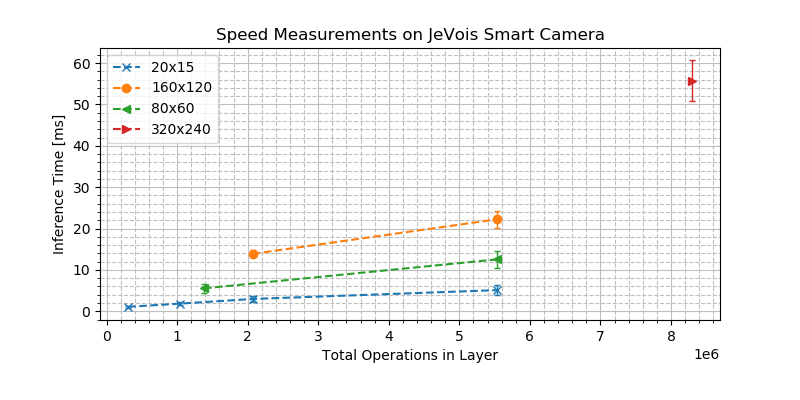
\includegraphics[width=0.8\textwidth]{fig/bottleneck_jevois}
	\caption{Inference Time of different layers on the JeVois. Each sample corresponds to the inference in a single layer. Dashed lines connect samples at the same resolution. It can be seen how an operation at a higher spatial resolution is significantly slower.}
	\label{fig:bottleneck_jevois}
\end{figure}

Hence, most speed can be gained when reducing the number of computations in the early layers where the spatial resolution is high. In \Cref{sec:object_detection} it could be seen that already a small amount of filters is enough to detect \acp{EWFO}. However, even evaluating 4 kernels at a resolution of 320x240 already takes 55 ms (\Cref{fig:bottleneck_jevois} red triangle). A total network of that size would require more than 200 ms and is thus too slow to be deployed in the control loop. Current research mostly addresses to reduce the computations when the convolved volumes are deep or the operations are performed on \acp{CPU} that do not support floating point operations. However, the bottleneck on the JeVois happens at small volumes and the hardware can perform floating point operations. Furthermore, \acp{EWFO} consist of thin elements that are spread over large parts of the image. Hence, we hypothesize that simply reducing the image resolution will lead to large drops in performance. An alternative is to increase the stride parameter in the early layers of the network. This reduces the number of locations at which the kernel is evaluated. \acp{EWFO} are sparse and spread over large parts of the image, while most of the image does not contain useful information. Hence, we hypothesize that increasing the stride parameter in the early layers will perform better than reducing the image resolution.

\section{Experiments}

In order to evaluate our hypotheses the network is trained with different architectures. Subsequently, performance and inference time on the JeVois are measured.

The JeVois supports aspect ratios of 4:3 and resolutions of 160x120, 320x240 and 640x480. Although, \ac{FCN} do not depend on the image resolution, the object appearance can change at lower image resolution. Hence, during training the images are scaled to 160x160 or 320x320 respectively. The anchor boxes are scaled in similar fashion. Finally, as the input image resolution decreases, the output grid size decreases by the same factor. This is not desirable as the output resolution should stay the same. Hence, when decreasing the input image to 160x160 we remove the last pooling layer such that the output grid stays at 20,20 or 10,10 respectively.

\section{Results}

\begin{figure}[hbtp]
	\centering
	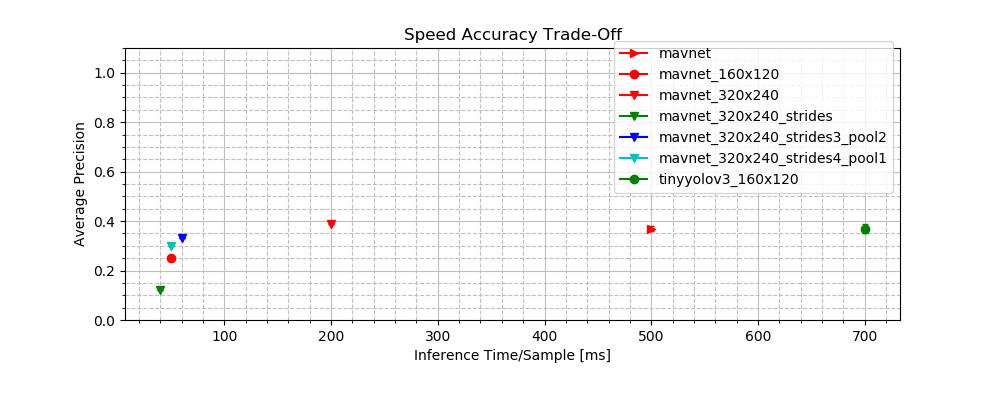
\includegraphics[width=0.8\textwidth]{fig/ap_speed_tradeoff}
	\caption{Inference Time of different layers on the JeVois. Each sample corresponds to a single layer. On the x-axis the total number of multiplications in that layer is displayed. It can be seen how an operation at a higher spatial resolution is significantly slower.}
	\label{fig:ap_speed_tradeoff}
\end{figure}

Due to their computational complexity deploying a \acp{CNN} on mobile devices is a challenging task

\section{Discussion}

\section{Conclusion}


In order to answer this question we measure the inference time of different model architectures. This enables us to investigate the bottlenecks and thus optimize the model architecture. The JeVois Smart Camera uses an aspect ratio of 4:3. Therefore we change the network resolution accordingly. The JeVois Smart Camera has only limited memory available. Using a network architecture that goes beyond the memory simply results in a system crash. For example our baseline network runs performs one network evaluation in 700 ms. This is at a resolution of 160x120.
\chapter{Discussion}

In this work we investigated a learning based approach for the detection of \acp{EWFO} on \acp{MAV}. The research was motivated by several drawbacks of the manual crafted detection method SnakeGate. The aim was to investigate whether a learning based Object Detector is more robust against, occlusion, out of view and changes in illumination. Our results show how the deep learning based detector outperforms SnakeGate especially in the cases of occlusion and out of view. The deep learning based detector can detect objects even when only 30\% of the object is visible or when backlight leads to strong changes in colour appearance.

Yet the deep learning based detector introduces its own drawbacks. For example the bounding boxes are generally less accurate than of SnakeGate. We assume that the reason is the general structure of \ac{Yolo}. \acp{CNN} collect "shallow" low level image features and combine them to a more deep representation of the image. Pooling layers reduce the spatial resolution to keep the number of computations tracktable, however thereby also local information about the features gets lost. In the final layers information is present which features are present in that part of the image, however it is not clear where they come from. 

This not only leads loss in localization accuracy but also to lack of transparency. In some scenarios a clearly visible gate is not detected by the \acp{CNN}. In this case it is hard to find out what part of the input image led to this wrong decision. In contrast for a simple algorithm such as  \textit{SnakeGate} it is clear at all times which input information led to a decision.

 Future work should address how to reflect back from the deep representation to the low level features.

A main argument for deep learning detectors is the fact that they can be trained on any kind of object and thus make feature engineering unnecessary. Furthermore, the learned representation are often much better than the features crafted manually. A drawback is the computational requirements of \acp{CNN}. For this work no training data was available and the computational requirements were limited. By implementing a data generation pipeline and refining the architecture we could show how the deep learning based method outperforms the manually crafted one. However, this process was a vast amount of work and yet we have a severe drop in peformance between the simulated and the real data. Hence, we have to wonder whether it would have not been more fruitful to invest time in feature engineering based on real data. It is questionable whether this is method would still perform better than the deep learning method. And yes for a new object it would required to be changed. But it would lead to a more transparent detector.
\todo{deep detector can be better extended but we loose track of whats going on, deep learning makes sense with the appropriate hardware and the appropriate data}
\chapter{Conclusion \& Future Work}
\label{sec:conclusion}
This work investigated the detection of \acp{EWFO} on \ac{MAV} using a \ac{CNN}. In this section a final discussion is given and a conclusion is derived. Furthermore, the research questions are answered and possible future work is discussed.


The research was motivated by the promising results of Deep Learning based Object Detectors and several drawbacks of manually crafted algorithms for the detection of racing gates in \ac{MAV} races. As the manually tuned features prove to be sensitive to light changes as well as to object occlusion, the aim was to investigate a more robust method. 

As no real training data were available, images and corresponding object labels were created with a simulator in order to train the \acp{CNN} based Object Detector \textit{YoloV3}. We hypothesized that due to the simple shape of \acp{EWFO} a small network should be able to learn the detection task. This led to the two research questions of this work which are now answered based on the conducted experiments.

\begin{enumerate}
	\item[\textbf{RQ1}]How can data be generated to train an object detector for \ac{EWFO} detection on a \acp{MAV}?
	
	It could be seen how the detector is sensitive to overfit to environmental conditions present in the training set. When testing a detector in a different simulated environment than the training set, the performance deteriorates between 30\% and 70\%. It was further investigated how to make the detector more invariant against such environmental changes. The results show how the variance in background is less important than the creation of realistic light conditions in the training set.
	
	When a wide range of view angles is introduced in training and test sets, the performance drops particularly for larger objects. It seems the detector has difficulties learning the detection from many angles. Better performance can be achieved by reducing the number of view angles in the training set. As this raised the question of how to create realistic view points, we proposed to simulate a flight through a race court. This way the created samples resemble the real world better. Even on unseen race courts, the detector achieves a precision of 70\% compared to the 20\% achieved by the network trained without simulating a flight. 
	
	Both methods of view point generation \todo{here you mention "both methods", but you didn't mention the 2 before in the conclusion} lack of control about the actual samples present in the training set. It is hard to think about all the view points that are required to train the network for a \acp{MAV} race. However, more control about the view points could give more insights about how the detector performs with different view angles in training and test set. Hence, future work could extend the data generation tool with more control about the view points and to conduct further experiments in that respect.
		
	In order to transfer the detector to the real world, it was found that image augmentation is crucial. Particularly modelling distortion improved the results on the real data. Yet there remains a gap between the results obtained in simulation and on real data. It cannot fully be resolved whether this is because of the complexity of the real data, or whether there are certain properties missing in the data generation process. Future work could address this issue by including real data in the training process. If this improves the results significantly, the problem is likely because of a reality gap. Otherwise, there might be a more fundamental problem in the chosen detector/complexity of the test set.
	
	In summary, we propose to fully synthesize environments when creating training data for the detection of \acp{EWFO} on \acp{MAV}. Furthermore, the precision can be improved by training the detector based on view angles it will see in the real world, possibly by simulating the flight behaviour. In order to transfer the detector to the real world, we recommend to use image augmentation. Particularly augmenting the images by modelling lens distortion improves the performance on the investigated dataset.

	\item[\textbf{RQ2}]How can \acp{EWFO} be detected using a \acp{CNN} on a \acp{MAV}?
	
	The \textit{YoloV3} can be adapted to the detection of \acp{EWFO}. The experiments showed how the detector can be confused by structures that are present within the empty part of the object. This was resolved by providing samples from different backgrounds and light conditions. We hypothesized that many backgrounds are required to achieve background invariance. However, the experiments showed that a small number of different environments is already enough to make the detector more robust against such confusion.
		
	A general drop of recall was observed for closer objects. It can be assumed that this is because it is more likely that object parts are out of view when the object comes closer. For the detection of racing gates on \acp{MAV} this result can be taken into account in later stages of the control loop. For example by using a dedicated detector for closer gates and combining the information. \todo{and by including a confidence value of the predictions into the control loop?} For the general detection of \acp{EWFO}, this result is interesting. Despite being clearly visible for a human, the detector struggles in some examples. Further experiments could include investigating how the performance changes when the detector is trained without any context such as the object pole.
	
	As \acp{EWFO} consist of relatively simple features, we hypothesized that a small network should be able to learn the task. The results showed that a shallow network of 9 layers performs equally well than a network with 15 layers. However, further reducing depth gradually reduces performance from 51\% to 35\%. When reducing the width of a network with 9 layers it can be seen how the performance slowly deteriorates from 51\% at its original size to 38\% to a fraction $\frac{1}{16}$ of its original size. 
	Hence, we conclude that a minimum of 9 layers is required if detection performance is the most important metric.
	
	For the detection of \acp{EWFO} on \acp{MAV} computational resources are more important. Our results show that a network with only one filter in the first layer can still achieve 38\% average precision. Hence, by reducing the network size to 0.4\% of its original size the performance drops only by 13\% average precision.\todo{do you have numbers to indicate the speed increase in this case?}
	
	The reduction of network size was taken out by retraining the network with a thinner architecture. An alternative way of reducing the network size is to apply \textit{Knowledge Distillation} (\Cref{sec:background}). This method showed promising results on deeper network. In future work it could similarly be applied for the detection of \acp{EWFO}.
	
	The trained detector was deployed on an example \ac{MAV}. The results show how by reducing the resolution the inference time can be increased significantly. However, the costs in terms of average precision are large. Instead we propose to remove pooling layers and to use layers with larger strides. This parameter allows to trade-off between average precision and inference speed. \todo{do you have numbers showing that? or references?}
	
	An alternative way to increase the network speed is \textit{weight quantization} (\Cref{sec:background}). As the target system of this work supports floating point multiplications, we did not further consider it. However, with an adequate low level implementation this could still lead to further speed up and should be investigated in future work.
	
	In a nutshell, it could be seen that a small network is able to learn the task. The inference time of the detector can be further increased without loosing too much performance. Finally, replacing pooling layers by convolutions with larger strides allows to trade-off between detection performance and inference speed.
		
\end{enumerate}

\todo{maybe add a short summary of your contributions: you have a trained CNN for efficient detection on MAV, you have recommendations on dataset construction and on CNN optimization, you can infer from the detailed analysis of the experiments results (all the bins you made) the limitations of your detector but that is not really an "issue" because you can use this info in the control loop}

Based on the experiments a detector could be developed and compared against the baseline. The experiments showed an improvement of performance compared to \textit{SnakeGate} of up to 16\% average precision, leading to a total of 32 \% $ap_{60}$. This improvement is mainly obtained in cases of difficult light conditions or occlusion. Hence, it can be concluded that indeed the \acp{CNN} can work better in such situations.

A network of similar complexity achieves 41\% $ap_{60}$ on a simulated data set which contains more objects and more difficult view angles. Therefore it can be seen that the potential of the learning based detector is much higher. Yet transferring the detector to the real world proves to be difficult, despite the relatively simple features of \acp{EWFO}. In some cases the object is clearly visible but not detected by the \acp{CNN}. These results show the general drawback of Deep Learning based approaches. It is not transparent why the objects are not detected and what exactly was learned by the network.

A frequent argument for Deep Learning is that it does not require cumbersome Feature Engineering. In this work, this step was technically replaced by Data Engineering and yet the remaining reality gap is high and some results are hard to understand. We have to ask ourselves if the lack of transparency, the amount of required data as well as the computational requirements are really worth the results gained in detection performance. \todo{haha, that's a pretty negative formulation.....}

Nevertheless, this work serves as a baseline for future work. The initial experiments show how a small amount of environments is already enough to make the detector relatively invariant against background. These results should apply similarly to the real world. Hence, it is not too much work to create a real world training set, and the data could be augmented with the data created in this work.

Furthermore, the experiments show trade-offs in speed and detection performance. The results can be used to design a detector for \acp{EWFO} based on available hardware and project requirements.





%\section{Method}
\label{sec:method}


\input{chapters/03_method/model}
\chapter{Transfer Learning}
\label{sec:training}

Supervised machine learning relies on the assumption that a hypothesis $h$ can be learned from a limited set of samples $X$ with their corresponding set of labels $Y$. The goal is to learn $h$ from a source set $D_s = \{X_{s},Y_{s}\}$ such that it can be applied on a target set of unknown examples $D_t = \{X_{t}\}$ to obtain the corresponding labels:

$$
h(X_t)\rightarrow Y_t
$$ 

Whether $h$ is performing well, can evaluated by splitting the labeled set of $D_s$ in a training set $D_{train}$ and test set $D_{test}$. $h$ is learned using the full information of $D_{train}$ and applied on the $D_{test}$. By evaluating a performance metric $m_A$ on $D_{train}$ information about the representation strength of $h$ can be inferred. The performance metric $m$ on $D_{test}$ gives an estimate of the performance of $h$ on $D_t$. Comparing $m_A$ and $m$ allows to evaluate whether model and dataset are suitable for the task.
			
This basic supervised machine learning setting relies on the assumption that $D_s$ follows the same i.i.d distribution as $D_t$. However, this can not be assumed for the application of this thesis. As most of the data is artificially created it will share properties with the real data but only to the extent that they can be modeled during creation. For example a graphic engine can not fully capture visual properties of all materials and light sources. Furthermore, is this model developed for application in locations with unknown light conditions and object variances that can be significantly different to the ones used at training time. When the source domain $S$ only shares a subset of properties with the target domain $T$ this is also referred to as a domain shift scenario. 


Learning models in such an environment is concerned by the field of Transfer Learning. The goal is to find a concept $h$ that performs best in the target domain $T$. Similar to $m_A$ and $m$ the performance $m_s$ in $S$ and the performance $m_t$ in $T$ can be used to evaluate whether a suitable model/dataset has been chosen/is available.

The task of learning from synthetic data can be summarized in:

$$
\text{arg}\max\limits_{h,S} m_t
$$

The goal is to create source domain $D_s$ and find a concept $h$ that maximizes its performance in the target domain $m_t$. This formulation yields two levels at which the domain shift problem can be addressed: (1) focusing on generating data or (2) focusing on finding a hypothesis that maximizes the performance.

In this thesis two types of domain shifts are considered: (1) A semi-supervised domain shift between synthetic data and real images. This means $D_s$ is available in large quantity, namely it is generated by a graphical engine. For $D_t$ a considerably smaller amount of labels is available \todo{describe real datasets}. 
(2) An unsupervised domain shift when environment conditions at test time can be significantly different to the ones at training time. In this case information about $D_t$ is only available as graphical models of the object of interest and several images of the domain. \todo{double check is this really an unsupervised domain shift since we dont even know X}

The conducted research is limited to \ac{CNN}-based object detection as they are investigated in this thesis. The chapter focuses on domain adaption while the exact model is described in \autoref{sec:object_detection}.

The relevant question to be investigated in this chapter is the following:

\begin{center}
	\textbf{How can data be generated to train a model for wire frame object detection?}
	\textbf{How can the model be made robust against domain shifts?}
\end{center}

The first question will be answered by choosing a state of the art method for object detection and training it with varying properties in $D_s$. By evaluating $m_s$ on synthetic data and $m_t$ on real images the influence of these properties will be measured.  

The second question will be answered by simulating a domain with synthetic data. That is the model will be trained in a room with significant different environment properties $D_s$ from the room it is tested in $D_t$.

The remaining parts of this chapter are structured as follows: \autoref{sec:training:related} discusses relevant related work. Based on the gained insights \autoref{sec:training:hypothesis} formulates several hypotheses to be investigated. \autoref{sec:training:experiments} outlines the experiments conducted to evaluate the formulated hypotheses. \autoref{sec:training:results} describes the obtained results. \autoref{sec:training:conclusion} discusses the results and answers the research question.

\section{Related Work}
\label{sec:training:related}

Domain shifts have been intensively studied in Machine Learning. 

A recent work \cite{Chen2018c} concerns the domain shift for object detection with deep neural networks. Based on the $\mathcal{H}$-Divergence \cite{Ben-David2010} domain classifiers are included in the network on the higher order feature activations. By incorporating the classifier in the training process and using a gradient reverse layer \todoref{gradient reverse} the feature activations are forced to be more similar. This enables to perform feature alignment in and end-to-end training process.

\cite{Xu2017} incorporate the domain adaptation by adversarial training. In a first step the network is trained using samples for the target and source domain. The obtained feature extractor is used to train a domain classifier. Finally the feature extractor is updated by inverting the domain classifier loss function and thus aligning the feature extractors.

\cite{Inoue} use variational auto encoders to create synthetic images.

\cite{Rozantsev} estimate parameters from real images to render synthetic images.

\cite{Peng2017} includes task-irrelevant samples and a source classifier to make the final network robust (?). Called zero-shot domain adaptation as no samples of the target domain are required.

\cite{Liu2018a}

\cite{Peng} use 3D CAD-models to augment the data during training.

Incorporating Camera Effects:
\cite{Carlson2018}
\begin{itemize}
	\item heaps of references in how camera properties influence object detectors
	\item introduces image augmentation pipeline based on physical model: chromatic aberration, blur, exposure, noise and color shift
	\item input parameters are modelled by hand, then randomly selected within "realistic" range
	\item no lense distortion
	\item method seem to benefit for small objects and when oversaturation applies due to camera effects
\end{itemize}


\cite{Vass}

Image Augmentation
\cite{Bai2017},

\ac{DR} was initially introduced by \cite{Tobin2017} for object localization. In contrast to domain adaptation approaches the method does not try to model the domain shift. Instead large variability in the source domain shall enable the model to learn a robust representation that is domain agnostic. \cite{Tremblay2018a} extends the approach to object detection.

The data is generated by a graphical engine. The following properties of the scene and the object are varied \cite{Tremblay2018a}:

\begin{enumerate}
	\item number, type and texture of objects of interest
	\item number, types, colours, scales of irrelevant objects (distractors)
	\item background image
	\item camera pose
	\item light sources
	\item visibility of ground plane
\end{enumerate}

An advantage of \ac{DR} is its ease of implementation and use, no assumptions about the target distribution have to be made neither are samples or labels of the target domain required. However, the method can fail to capture important patterns if the randomization is too strong. For example the movement pattern of a \ac{MAV} is ignored when placing the camera randomly.
 
\section{Approach}
\label{sec:training:hypothesis}

While a lot of approaches discussed in \autoref{sec:training:related} aim to learn a general representation that works across domains, other approaches try to incorporate more target domain knowledge to improve performance. 

It is to expected that there is a trade-off between generalization and specialization. For example placing the gates align only in positions that are physically possible allows the model to pick up context cues and thus should simplify the learning problem. Although, such a model will maybe not be able to detect objects at random positions, it is likely to never see them in the real world. 

On the other hand if the light conditions are limited to a certain room the model is likely to perform well there but will fail as soon as applied in another room. Therefore, what patterns the model is variant and invariant to is a design choice depending on the application.

The more general the model has to be, the poorer it might perform in a specific domain or the more complex it has to be. On the other hand a much simpler model can be used if particular properties are chosen to be embedded in the training domain. \todo{mention bias variance trade off here?}

This leads to the formulation of two hypothesis to be investigated:

\begin{enumerate}
	\item[H1] The more similar the properties between $D_s$ and $D_t$ the higher $m_t$ of a fixed model.
	\item[H2] The less similar the properties between $D_s$ and $D_t$ the more complex a model has to be to keep $m_t$.
\end{enumerate}



\section{Experiments}
\label{sec:training:experiments}

The experiments conducted

Initially those domain properties are investigated that can be controlled when creating the training data. The domain shift between synthethi
\begin{enumerate}
	\item \textbf{Background.} 
	
	Background refers to how the object is embedded in the environment. For example if synthetic objects are placed on random backgrounds this will not necessarily represent the background in the real world.
	
	The property can be influenced when creating the object scene: (1) The objects can be placed on randomly selected images, (2) The background can be chosen according to some properties, e.g. their similarity to the target domain. (3) A full scene can be rendered when creating data.
	
	\item \textbf{Object Placement.} 
	
	Object placement refers to the object's location in the scene. For example one would not expect an apple placed at the ceiling of a room.
	
	This property can be controlled when placing the images in background: (1) The objects can be placed at a random location on the background. (2) The objects can be placed similarly as in the target domain.
	
	\item \textbf{Illumination.} 
	
	Light conditions can influence the object appearance and its background.
	
	This property can be controlled by the graphic engine: (1) A sun-like light source can be used that spreads equally across the scene. (2) More particular light sources can be used e.g. for simulation artificial indoor light.
	
	
	\item \textbf{Camera Placement.} 
	
	Camera placement refers to the view point of the camera. For example on an \ac{MAV} the view point is limited within a range where it is still possible to fly. Randomly placing the camera does not capture such patterns.
	
	This property can be controlled when synthesizing data: (1) The camera can be placed randomly in the scene, as long as the object is still visible. (2) The camera can be placed based on the expectations in the target domain. (3) The camera can be placed following a physical model of a drone.
	
	\item \textbf{Camera Properties.} Camera properties refers to the intrinsic camera parameters. For example lens distortion can significantly influence the appearance of an object.
	
	(1) Random properties (2) Camera model, distortion model.
	
	\item \textbf{Noise.} Noise can be created by different sources. For example is noise introduced by the sensor, but also by camera motion.
	(1) Gray/Colour noise (2) Motion blur
	
\end{enumerate}

\todo{Prepare a synthetic dataset of several rooms}
\todo{Prepare a real dataset of at least two rooms}

\todo{Mesaure similarity between generated set and real set: label distribution (h,w, location, angles), domain(?), h divergence}

\todo{Quantify each property. Make a plot performance vs more effects}



\section{Results}
\label{sec:training:results}

\section{Conclusion}
\label{sec:training:conclusion}

%\section{Summaries}
%\subsection{Modeling Camera Effects to Improve Deep Vision for Real and Synthetic Data\cite{Carlson2018}}
%


\chapter{Transferring it to the Real World}
\label{sec:tradeoff}


After having created a set of 2D images, the final step applies low-level image transformations. It allows to further simulate sensor effects and increase the variance in the generated data.

In literature \cite{Krizhevsky2012a,Howard2013,Redmon,Liu} the application of image augmentation is a common tool to improve the detection performance. The experiments in \cite{Carlson2018} show how the incorporation of sensor effects particularly improves the performance of models learned on fully synthesized data. In the \ac{MAV} domain sensor and lens effects have a significant influence on the obtained sample. Hence, we hypothesize that the incorporation of these effects is particularly useful for the \ac{MAV} domain.

\paragraph{Lens Distortion}

Lens distortion is a form of optical aberration which causes light to not fall in a single point but a region of space. For \acp{MAV} commonly used wide-angle lenses, this leads to barrel distortion and thus to straight lines appearing as curves in the image.

The effect is applied using the model for wide-angle lenses from \cite{Vass}. It models the removal of lens distortion as combination of radial and non-radial part, that is approximated with a second order Taylor expansion:
\todo{double check formula is (y in first line?)}
\begin{equation}
f(x,y) =
\begin{pmatrix}
x (1 + \kappa_1 x^2 + \kappa_1 (1 + \lambda_x) y^2 + \kappa_2(x^2 + y^2)^2) \\
y (1 + \kappa_1 x^2 + \kappa_1 (1 + \lambda_y) y^2 + \kappa_2(x^2 + y^2)^2)
\end{pmatrix} 
\label{eq:distortion}
\end{equation}
Where:
\begin{itemize}
	\item f yields the undistorted coordinates.
	\item $\kappa_1$ $\kappa_2$ control the radial distortion 
	\item $\lambda_x$ and $\lambda_y$ control the tangential distortion
\end{itemize}

Applying the lens distortion to an image is done using the inverse of \Cref{eq:distortion}. However, as there is no closed form solution, so the Newton-approximation.

An example with $\kappa_1 = 0.5, \kappa_2 = 0.5$ is displayed in \Cref{fig:distortion}. It can be seen how the previously straight lines appear as circular shape.

\paragraph{Chromatic Aberration.}

Chromatic Aberration is caused when different wavelengths of light do not end up in the same locations of the visual sensor. This leads to a shift in the colour channels of the image.

Similarly to \cite{Carlson2018}, chromatic aberration is applied by scaling the locations of the green channel, as well as applying translations on all channels. The model can be implemented as affine transformation of the pixel locations for each channel:

\begin{equation}
f(x_C,y_C) = \begin{pmatrix}
S & 0 & t_x \\
0 & S & t_y \\
0 & 0 & 1
\end{pmatrix} \begin{pmatrix}
x_C \\
y_C \\
1
\end{pmatrix}
\end{equation}

Where $C$ is one colour channel of the image.

An example is displayed in \Cref{fig:chromatic}. It can be seen how the red and green channel are shifted relative to each other. Thus two bars appear in the image.

\paragraph{Blur}

Motion noise is caused when light falls in different locations of the images sensor due to a fast movement of the camera. It leads to blurry images based on the sensor motion.

The phenomenon depends on camera properties as well as the motion of camera and objects. Although a full modelling of this process might benefit the learning process, it requires a complex pipeline and is computationally expensive. Therefore a strong simplification is used, namely a one-dimensional Gaussian filter:

An example for vertical blur is displayed in \Cref{fig:motionblur}. It can be seen how particularly horizontal lines appear softer.

Next to motion, sensor noise can lead to blurry images. For the blur operation a 2D Gaussian kernel is applied on the input image with:

\begin{equation}
k = \frac{1}{2\sigma_x\sigma_y\pi}e^{-\sqrt{\frac{x^2 + y^2}{2\sigma_x\sigma_y}}} 
\end{equation}
\todo{double check notation}
\paragraph{Exposure.}

Exposure is the time the sensor records light in order to create an image. Over- and Underexposure are caused when this time is too short or too long, leading to too dark or too bright images.

Following the model from \cite{Carlson2018}:

\begin{equation}
f(S) = \frac{255}{1 + e^{-A S}}
\end{equation}
where $A$ is a constant term for contrast and $S$ the exposure.
\todo{whats a}
The image can be re-exposed with:

\begin{equation}
I' = f(S+\Delta S)
\end{equation}

where $S$ is obtained from :
\begin{equation}
S = f^{-1}(I)
\end{equation}

An example for overexposure is displayed in \Cref{fig:exposure}. It can be seen how lighter areas appear particularly light, while dark areas remain dark.

\subsection{Color Variations}

\todo{describe hsv scaling}


\begin{figure}[htbp]
	\centering
	\begin{minipage}{0.33\textwidth}
		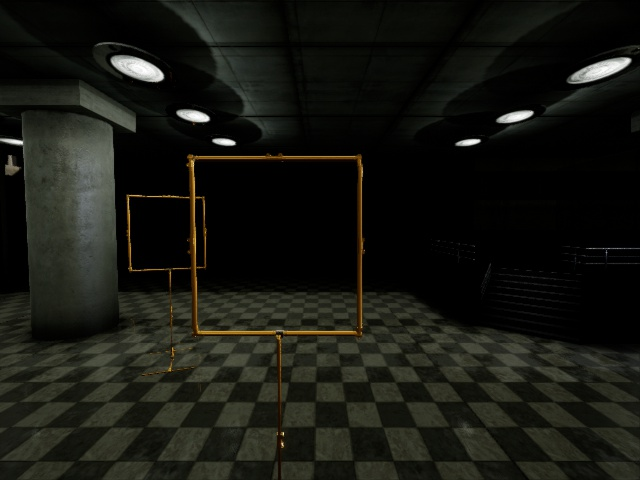
\includegraphics[width=\textwidth]{fig/gate_example}
		\caption{Original Image.}
		\label{fig:orig}
	\end{minipage}
	\begin{minipage}{0.33\textwidth}
		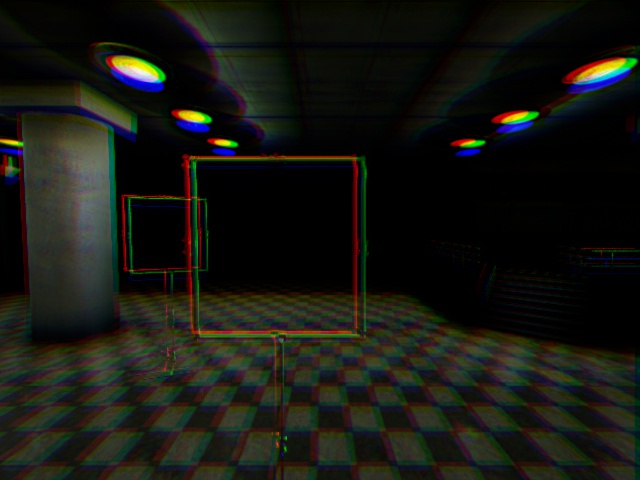
\includegraphics[width=\textwidth]{fig/gate_example_chromatic}
		\caption{Chromatic Aberration.} 		
		\label{fig:chromatic}
	\end{minipage}
	\begin{minipage}{0.33\textwidth}
		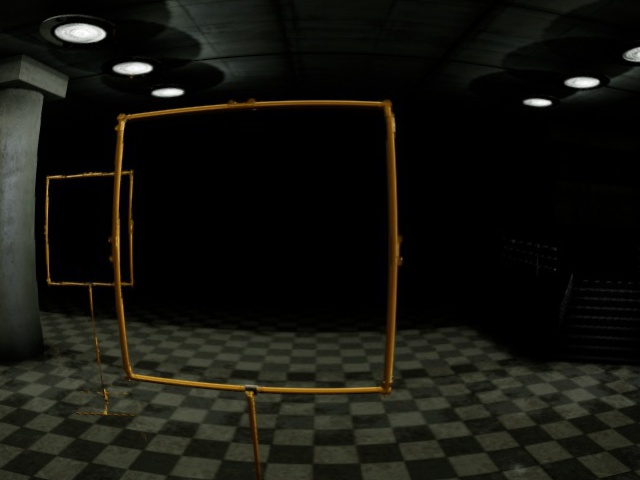
\includegraphics[width=\textwidth]{fig/gate_example_distorted}
		\caption{Lens Distortion. }		
		\label{fig:distortion}
	\end{minipage}
	
	\begin{minipage}{0.33\textwidth}
		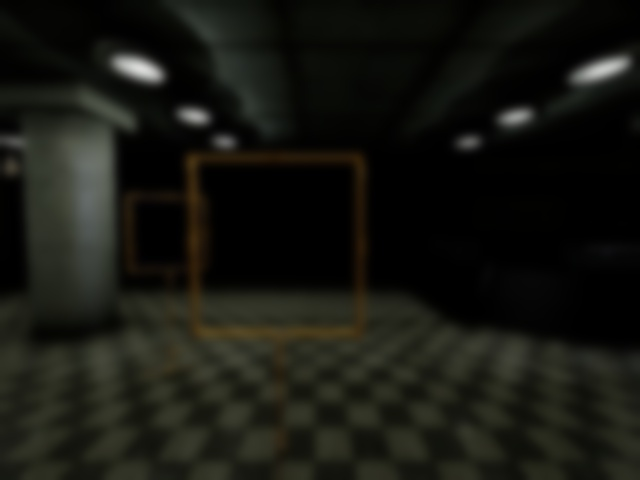
\includegraphics[width=\textwidth]{fig/gate_example_focusblur}
		\caption{Out-of-Focus blur.}
		\label{fig:focusblur}
	\end{minipage}
	\begin{minipage}{0.33\textwidth}
		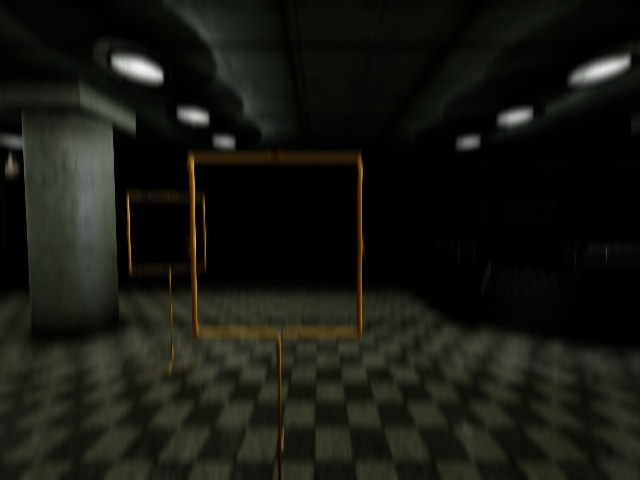
\includegraphics[width=\textwidth]{fig/gate_example_motionblur_v}
		\caption{Vertical Motion Blur.}
		\label{fig:motionblur}
	\end{minipage}
	\begin{minipage}{0.33\textwidth}
		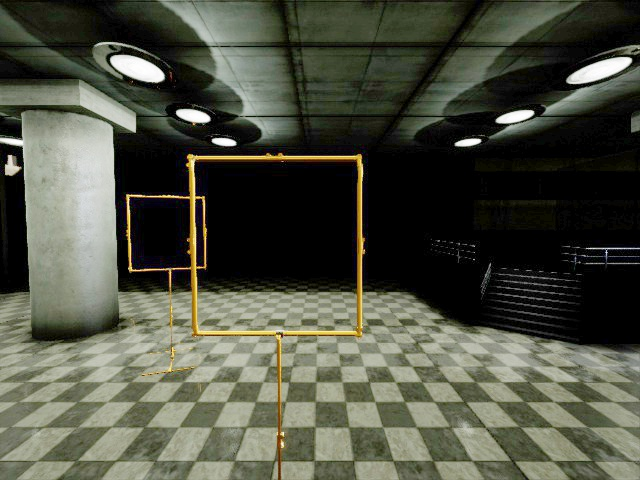
\includegraphics[width=\textwidth]{fig/gate_example_exposure}
		\caption{Exposure.}
		\label{fig:exposure}
	\end{minipage}
\end{figure}

\subsection{Hypothesis}
\label{sec:training:hypothesis}

This chapter summarizes the hypotheses formulated in the previous chapters:

\begin{enumerate}
	\item[$\mathcal{H}_1$] An object that is not empty and provides a more distinctive structure is less background dependent than an \ac{EWFO}.
	
	\item[$\mathcal{H}_2$] The incorporation of correct placement/light conditions improves the performance of a model trained to detect \acp{EWFO}.
	
	\item[$\mathcal{H}_3$] The incorporation of a camera motion model resembling the target domain improves the performance of a model trained to detect \acp{EWFO}. 
	
	\item[$\mathcal{H}_3$] Including sensor effects present in the target domain, improves the performance of a model trained to detect \acp{EWFO}. 
	
\end{enumerate}



\section{Experiments}
\label{sec:training:experiments}
In order to evaluate the formulated hypotheses several experiments are conducted. The model used is the TinyYoloV3-Architecture, further described in \Cref{sec:object_detection}. The reported metrics are described in \Cref{sec:metrics}. For all experiments mean and standard deviation of 5 runs are reported.

For the random view point generation the following parameters are used:

\begin{equation}
x = \mathcal{U}(-30,30),\quad y = \mathcal{U}(-20,20),\quad z = \mathcal{N}(-4.5,0.5)),\quad
\phi = \mathcal{U}(0,0.1\pi),\quad \theta = \mathcal{U}(0,0.1\pi),\quad \psi = \mathcal{N}(-\pi,\pi)
\label{eq:distroexp}
\end{equation}
Where $ \mathcal{U}(a,b)$ is a uniform distribution between $a,b$ and $\mathcal{N}(\mu,\sigma^2)$ is a Gaussian distribution with mean $\mu$ and variance $\sigma^2$.

The parameters are chosen experimentally aiming to resemble common view points of a person standing in the room.

\subsubsection{Experiment I}
The empty space of an \ac{EWFO} is augmented with a detailed texture. An example can be seen in \Cref{fig:cats}.
\begin{figure}
	\centering
	\includegraphics[height=5cm]{fig/cat}
	\caption{The \ac{EWFO} is augmented with a detailed texture.}
	\label{fig:cats}
\end{figure}

The object is placed in a scene with uniformly coloured backgrounds and a training set of 20 000 samples is created. In similar fashion a training set is created without the texture rich augmentation. The test set contains 1000 samples created in the \textit{IROS} environment by randomly placing the camera following \Cref{eq:distroexp}.




\subsubsection{Experiment II}

Several models are trained on 20 000 samples each.
\begin{itemize}
	\item[ModelU] Uniform
	\item[ModelSVE] Single Virtual Environment
	\item[ModelRB] Real Backgrounds
	\item[ModelVVE] Various Virtual Environments
	\item[ModelRBVVE] Real Backgrounds + Various Virtual Environments
\end{itemize}


\begin{table}[htbp]
	\caption{}
	\begin{tabular}{|l|l|l|l|r|r|r|l|l|l|}
		\hline
		& Validation Set &  &  & \multicolumn{1}{l|}{IROS2018} & \multicolumn{1}{l|}{} & \multicolumn{1}{l|}{} & Real Data &  &  \\ \hline
		& AP40 & AP60 & AP80 & \multicolumn{1}{l|}{AP40} & \multicolumn{1}{l|}{AP60} & \multicolumn{1}{l|}{AP80} & AP40 & AP60 & AP80 \\ \hline
		U &  &  &  & 0.05 & 0.01 & 0 &  &  &  \\ \hline
		SVE &  &  &  & 0.29 & 0.17 & 0.02 &  &  &  \\ \hline
		VVE &  &  &  & 0.61 & 0.49 & 0.17 &  &  &  \\ \hline
		RB &  &  &  & 0.42 & 0.28 & 0.04 &  &  &  \\ \hline
	\end{tabular}
	\label{tab:env}
\end{table}


\subsubsection{Experiment III}

Three models are trained: Model I using random placement, Model II using the drone motion model, Model III using a combination of both methods. In both experiments environment and light conditions as well as object locations are the same. The models are tested on two test sets: Set I created by randomly placing the camera. Set II by using the drone motion model, where a circuit is used that has not been part in the generation of the training data.


\subsubsection{Experiment IV}

In order to evaluate $\mathcal{H}_4$ the individual domain properties are measured on the target domain and incorporated in the training set.


\section{Results}
\label{sec:training:results}

\section{Discussion}
\label{sec:training:discussion}

\section{Conclusion}
\label{sec:training:conclusion}



%\chapter{Discussion}
\label{sec:disc}
\todo{answer research questions}
%% Use letters for the chapter numbers of the appendices.
%\appendix

\section{Data Generation}
\label{sec:appendix:datagen}

This section describes how the ground truth labels are obtained when generating data.

\subsection{Camera Model}

\hfill \\
The camera itself is modelled with the pinhole camera model that contains six parameters:

\begin{enumerate}
	\item Focal length $f_x,f_y$
	\item Central point $c_x,c_y$
	\item Sensor skew $s_x, s_y$
\end{enumerate}

The model can be summarized in the intrinsic camera matrix $C$:
\begin{equation}
C = \begin{bmatrix}
\frac{fx}{s_x} & 0 &cx \\
0&  \frac{f_y}{s_y}&cy \\
0& 	0&	1
\end{bmatrix}
\label{eq:pinhole1}
\end{equation}

The model projects 3D coordinates $X$ to the image plane following:
\begin{equation}
X' = C X
\label{eq:pinhole2}
\end{equation}
Where $X$ are points described in homogeneous coordinates originating from the cameras position.

For data generation several tools are used. 3D Models for the \ac{TO} are taken from ... OpenGl is used to render these objects and replace the background with a particular image. The Unreal Engine and AirSim are used to render a full scene.

Within the graphic engines, the objects can be placed in 3D space. From the known object shape the surrounding bounding box can be defined in 3D coordinates. Using the pinhole camera model described in \Cref{eq:pinhole1} the corresponding 2D coordinates on the image plane can be obtained with the following:

The camera position is described by its rotation matrix $R$ and its translation vector $t$. Where $R$ is obtained from the Euler angles with:
$$
R =
$$
The 3D coordinates of the objects relative to the camera can be obtained by applying the inverse transformation $T$ of $R$ and $t$ with:
$$
t' = R \times t
$$
$$
T = R^{-1}|-t'
$$
$$
X_{Cam} = T\times X
$$
The full projection can then be expressed by the matrix multiplication:
$$
X' = C\times T\times X
$$
Where $C$ is the intrinsic camera matrix defined in \Cref{eq:pinhole1}.

\bibliography{thesis}

\end{document}

